\documentclass[a4paper,10pt]{thesis}

\usepackage{amsmath}
\usepackage{amssymb}
\usepackage{graphicx}
\usepackage{makeidx}
\usepackage{fancybox}
\usepackage{theorem}

\title{Electromagnetic Waves in Space and the STEREO/SWAVES experiment}
\author{T.H. Oswald, BSc}

\makeindex
\index{STEREO}
\index{electromagnetic!waves}
\begin{document}

\maketitle

\newpage
\paragraph*{}
 \begin{verbatim}



















\end{verbatim}
\begin{center}
\framebox{\parbox[c]{12cm}{\emph{To Mary, who had and has to endure my frequent state of absentmindedness, when my mind wanders through the realms of physics.}}}
\end{center}
\frontmatter
\chapter{\textbf{Acknowledgments}}
Many people were involved in the successful creation of this thesis. Above all I thank Prof. H.O. Rucker who offered me to work on this subject and supported me with his great experience. I also thank my colleagues W. Macher and G. Fischer who never ran out of patience when I attacked them with countless questions. I am also deeply indebted to my wife Mary and my son Michael, who provided me with the necessary time to complete this task. Last but not least, I thank my parents, without whom this document would not exist in many respects.

\tableofcontents
\begin{abstract}
\paragraph*{}
The electromagnetic wave is one of the most important tools of a space scientist. The understanding of this tool is vital in our quest to extend our knowledge about space and the physics of space. This thesis deals with electromagnetic waves,\index{electromagnetic!waves} their properties and the possibilities to use them in the field of space science. The topics are selected, such that they are relevant for the STEREO \index{STEREO}mission, to be launched in the near future. Electromagnetic waves, in general, are discussed, with special emphasis on direction finding. At last, one of the methods for finding the effective length vectors, the numerical method,\index{numerical!method} is treated with regard to the STEREO spacecraft.\index{spacecraft}\\

\end{abstract}
\mainmatter
\chapter{\textbf{Introduction and Objectives}}

\paragraph*{}
Remote Sensing is a term that describes the procedure of gathering information remotely. Space science is one of the fields, where remote sensing is used all the time. Due to the hostile environment of space and the large distances involved, it is often the only possible way to extend the knowledge of these distant worlds. Remote sensing, in turn, relies heavily upon the use of electromagnetic radiation. Electromagnetic (EM) waves can be used to probe areas of space and celestial bodies, EM waves that are radiated by natural processes can be received by antennas and give valuable information about the mechanism that creates them and the area of space which lies between the origin and the antennas, and they can be used to relay the information back to earth or wherever it is required for further processing. Naturally, it is absolute necessary that we know how electromagnetic radiation behaves in space, how it can be generated, how it propagates through space and how it is influenced by the \index{plasma}plasma that is abundant up there.

\paragraph*{}
One of the space missions, currently in the last phase of preparation, is STEREO, conducted by \index{NASA}NASA and to be launched in spring 2006. The mission consists of two \index{space probes}space probes which will enter a \index{heliocentric}heliocentric orbit. One spacecraft will orbit \index{sun}sun ahead of the earth, the other behind.

\paragraph*{}
The scientific goal of the mission is to increase our knowledge of the physics of our \index{solar!system}solar system, especially:

\begin{itemize}
\item Understanding the causes and mechanisms of \index{CME}Coronal mass ejection (CME) initiation
\item Characterize the propagation of CMEs through the heliosphere
\item Discover the mechanism and sites of energetic particle acceleration in the low corona and the interplanetary medium
\item Develop a 3D time dependent model of the \index{magnetic!topology}magnetic topology, \index{temperature}temperature, density and \index{velocity}velocity structure of the ambient \index{solar!wind}solar wind
\end{itemize}

\paragraph*{}
Among several other experiments, one particular important is STEREO\\
WAVES (SWAVES). This experiment is designed to track interplanetary \index{radio bursts}radio bursts and trace the generation and evolution of radio disturbances from the sun to earth orbit \index{sun}\index{earth!orbit}and beyond. Each spacecraft has three, \index{antenna}nearly orthogonal, antennas. With this configuration, it is possible to perform \index{direction finding}direction finding to find the direction of the origin of the received radiation and information about its \index{polarization}polarization. When both spacecraft receive radiation from the same source at the same time, the actual location of the source can be pinpointed by the method of triangulation\index{triangulation}.

\paragraph*{}
The technique of direction finding relies heavily upon the precise knowledge of the direction and the length of the three antennas. Unfortunately, the real behavior of the antennas is different than one would predict for the geometric configuration of the antennas. The reason is the influence of the body of the spacecraft. The spacecraft surface is made of conducting material, so it can, in principle, be regarded as part of the antennas. As a result, each antenna behaves as if it would point into a slightly different direction, with a slightly different length. The vector that describes the direction and length of this virtual antenna is called effective length vector. This effective length has to be determined, before any direction finding can be conducted.

\paragraph*{}
There are three known methods to determine the effective length vectors of the antennas of a spacecraft:

\begin{enumerate}
\item The numerical approach\index{numerical!approach}
\item The experimental approach\index{experimental!approach}
\item In-flight calibration\index{in flight calibration}
\end{enumerate}

\begin{figure}
\begin{center}  % Requires \usepackage{graphicx}
  \includegraphics[width=12cm]{rheomodell.eps}\\
\caption{Rheometry model of the NASA/STEREO spacecraft}\label{fig_rheomod}
\end{center}
\end{figure}

\paragraph*{}
All three methods complement each other and are necessary components of the process of determination and validation of the antenna properties. However, subject of \index{antenna!propertiy}\index{Master Thesis}this Master Thesis is only the numerical method. For information about the rheometry, see
\cite{rheometry} or \cite{macher_dipl}. The model used for the experimental method can be seen in figure \ref{fig_rheomod}.

\paragraph*{}
The numerical method is realized by computer programs and consists of two steps. First, the distribution of the currents on the surface and the antennas is calculated. This distribution can be used to calculate the \index{effective length vector}effective length vectors and other antenna properties, like antenna impedances. This is the second step.\index{antenna!impedance}

\paragraph*{}
An analytical solution of the surface current distribution is normally impossible to find, owing to the complex structure of the spacecraft. This is the reason, why one has to rely on numerical methods. For this purpose, the surface of the spacecraft is modeled as a grid of wires with proper conductivities. As an example the wire grid model of Cassini, which was used to study the RPWS antennas (\cite{cassini},
 \cite{cassini2} and
 \cite{cassini3}). The geometrical data and information about the material is fed into the software packages performing the nescessary calculation. Theses software packages are Concept II and ASAP. The output of this computation is a matrix, describing the surface current distribution. This data is, in turn, the input of the next stage of the calculation, where the effective length vectors are computed.\index{RPWS}\index{Cassini}\index{numerical!method}

\paragraph*{}
The process of computing the effective length vectors involves the solving of a complicated surface integral. This is calculated by the Matlab routines of the ASAP toolbox. Detailed Information about this toolbox can be found in \cite{toolbox}, \cite{toolbox2}
and \cite{antenna_report_1} .\index{matlab}\index{ASAP toolbox}\index{effective length vector}

\paragraph*{}
The computation has to be performed for all three antennas and for both spacecraft of the STEREO mission. Since the two spacecraft do not have the same shape, a separate wire grid model has to be constructed for each. The whole calculation will be done several times with a slightly different configuration, to investigate the influence of particular parts of the spacecraft on the deviation of the effective antenna axis from the geometrical axis. Fortunately, the effective length vector is independent of frequency and direction of the incoming wave, as long as the antenna is short in relation to the wavelength, which is the frequency range, where the direction finding will be performed, thereby defining the constraint of the computation.\index{spacecraft}\index{STEREO}\index{wire grid}\index{effective antenna axis}
\paragraph*{}
The objective of this Master Thesis is to describe the mathematical formulation of electromagnetic radiation, discuss their propagation in space, especially with regard to the plasma that fills space, treat the generation of electromagnetic waves and their transmission and reception by the use of antennas, as far as it is applicable to space science, develop a formula apparatus for direction finding with three monopole antennas, and finally describe the process of finding the effective length vectors by numerical methods of the STEREO spacecraft. \index{Master Thesis}\index{propagation}\index{reception}\index{monopole antenna}\index{numerical!method}\index{direction finding}\index{space science}\index{electromagnetic!wave}

\chapter{\textbf{Electromagnetic Radiation: The Basics}}\index{electromagnetic!radiation}

\section{\textbf{Introduction}}

\paragraph*{}
When electromagnetic (EM) waves traverse space, they will meet plasmas of all kinds during their journey. The plasma effects the propagation of the waves. When working with EM waves in space, we can, sometimes, neglect these effects when doing calculations, but sometimes we can't.

\paragraph*{}
In this chapter, Maxwell's equations are taken as base to derive the wave equations for EM waves in vacuum. Then the effect of a medium, a lossy medium, plasma and magnetized plasma, are taken into account.\index{Maxwell!equation}

\section{\textbf{The plane wave solution in free space}}
\subsection{Monochromatic waves}
\paragraph*{}
Maxwell's equations form the basis.\index{Maxwell}\index{wave!monochromatic}\index{wave!solution}

\begin{eqnarray}
\nabla \cdot \mathbf{D}&=&\rho \label{maxwell1}\\
\nabla \cdot \mathbf{B}&=&0 \label{maxwell2} \\
\nabla \times \mathbf{E}&=&-\frac{\partial \mathbf{B}}{\partial t} \label{maxwell3} \\
\nabla \times \mathbf{H}&=&\mathbf{j}+ \frac{\partial \mathbf{D}}{\partial t} \label{maxwell4}
\end{eqnarray}

\paragraph*{}
This set of equations describes the relations between the sources, currents and charges, and the fields in the SI system. The fields are, in general, functions of time and position, but the brackets are omitted for easier readability. When postulating vacuum in free space, there are no source terms (charges and currents) and no interference due to the existence of matter, the equations can be simplified a bit.\index{units!SI}\index{vacuum}

\begin{eqnarray}
\nabla \cdot \mathbf{E}&=& \frac{\rho}{\varepsilon_0} \label{maxwell_freespace1}\\
\nabla \cdot \mathbf{B}&=& 0 \label{maxwell_freespace2}\\
\nabla \times \mathbf{E}&=& -\frac{\partial \mathbf{B}}{\partial t} \label{maxwell_freespace3}\\
\frac{1}{\mu_0}\nabla \times \mathbf{B}&=&\mathbf{j}+\varepsilon_0 \frac{\partial \mathbf{E}}{\partial t} \label{maxwell_freespace4}
\end{eqnarray}

\paragraph*{}
Additionally the constitutive equations are needed, which relate the two types of field to each other. In vacuum, the fields are related to each other by a constant.\index{constitutive equations}\index{vacuum}

\begin{eqnarray}
\mathbf{D} &=& \varepsilon_0 \mathbf{E} \label{constitutive_1_vacuum} \\
\mathbf{B} &=& \mu_0 \mathbf{H} \label{constitutive_2_vacuum}
\end{eqnarray}

\paragraph*{}
The constants are the permittivity and permeability of free space and have the following values.\index{permittivity}\index{permeability}

\begin{eqnarray}
  \varepsilon_0 &=& 8.8542 \cdot 10^{-12} farad \cdot m^{-1} \\
\mu_0 &=& 4 \pi \cdot 10^{-7} henry \cdot m^{-1}
\end{eqnarray}

\paragraph*{}
In linear media, when $\varepsilon$ and $\mu$ are functions of position and time\footnote{but \textbf{not} of field strength}, the constitutive equations can be written as:

\begin{eqnarray}
\mathbf{D} &=& \varepsilon (\mathbf{r},t) \mathbf{E} \label{constitutive_1_linear} \\
\mathbf{B} &=& \mu (\mathbf{r},t) \mathbf{H} \label{constitutive_2_linear}
\end{eqnarray}

\paragraph*{}
In both cases, the principle of superposition applies. This property simplifies the problem solving process immensely. When exposed to high electric or magnetic fields, all media become non-linear, even vacuum, when the energy density approaches a value close to the point where fundamental particles are created.\index{superposition}

\paragraph*{}
In vacuum, when no charges and currents exist, Maxwell's equations can be further simplified.\index{Maxwell!equation}

\begin{eqnarray}
\nabla \cdot \mathbf{E}&=& 0 \label{maxwell_freespace_nosource_1}\\
\nabla \cdot \mathbf{B}&=& 0 \label{maxwell_freespace_nosource_2}\\
\nabla \times \mathbf{E}&=& -\frac{\partial \mathbf{B}}{\partial t} \label{maxwell_freespace_nosource_3}\\
\nabla \times \mathbf{B}&=& \varepsilon_0 \mu_0 \frac{\partial \mathbf{E}}{\partial t} \label{maxwell_freespace_nosource_4}
\end{eqnarray}

\paragraph*{}
These equations, can be manipulated in a way that they end up as wave equations for both fields. One has to take the curl of equation (\ref{maxwell_freespace_nosource_3}) and substitute (\ref{maxwell_freespace_nosource_4}) to eliminate \textbf{B}.\index{wave!equation}

\begin{eqnarray}
\nabla \times \nabla \times \mathbf{E}&=& -\nabla \times \frac{\partial \mathbf{B}}{\partial t} \\
\Rightarrow \nabla ( \nabla \cdot \mathbf{E})- \nabla^2 \mathbf{E} &=& - \varepsilon_0 \mu_0 \frac{\partial^2 \mathbf{E}}{\partial t^2}
\end{eqnarray}

\paragraph*{}
Remembering that the divergence of the electric field must vanish in a source free environment, one gets

\begin{equation}\label{wave_equation_E}
\nabla^2 \mathbf{E}-\varepsilon_0 \mu_0 \frac{\partial^2 \mathbf{E}}{\partial t^2}=0
\end{equation}

\paragraph*{}
A comparable manipulation to the magnetic field yields.

\begin{eqnarray}
\nabla \times \nabla \times \mathbf{B}&=& \varepsilon_0 \mu_0 \nabla \times \frac{\partial \mathbf{E}}{\partial t} \\
\Rightarrow \nabla ( \nabla \cdot \mathbf{B})- \nabla^2 \mathbf{B}&=& -\varepsilon_0 \mu_0  \frac{\partial^2 \mathbf{B}}{\partial t^2}
\end{eqnarray}

\paragraph*{}
The divergence of the magnetic induction is, not only in source free space, but generally zero. Hence

\begin{equation}\label{wave_equation_B}
\nabla^2 \mathbf{B}-\varepsilon_0 \mu_0 \frac{\partial^2 \mathbf{B}}{\partial t^2}=0
\end{equation}

\paragraph*{}
These wave equations can be solved. The most general solution is d'Alambert's solution, which has the following form  in case of the electric field.\index{d'Alambert solution}

\begin{equation}\label{dAlambert}
\mathbf{E}=\mathbf{E_0}\mathfrak{F}(\mathbf{k}\cdot \mathbf{r} - \omega t)
\end{equation}

\paragraph*{}
$\mathfrak{F}$ is any function of the argument $\mathbf{k}\cdot \mathbf{r}-\omega t$, where $\mathbf{E_0}$ points in the direction of the electric field and \textbf{k} is the wave vector, which points in the direction of the wave propagation. A second requirement must be fulfilled, the solution must also obey (\ref{maxwell_freespace_nosource_1})\index{wave!propagation}.

\begin{eqnarray}
    \nabla \cdot \mathbf{E}&=& \nabla \cdot \mathbf{E_0}\mathfrak{F}(\mathbf{k}\cdot \mathbf{r}-\omega t)\\
&=& \mathbf{E_0} \cdot (k_x\mathbf{\hat{x}} + k_y\mathbf{\hat{y}}  + k_z \mathbf{\hat{z}} ) \mathfrak{F}(\mathbf{k}\cdot \mathbf{r}-\omega t) \nonumber \\
&=& \mathbf{E_0} \cdot \mathbf{k} \mathfrak{F}(\mathbf{k}\cdot \mathbf{r}-\omega t) = 0\nonumber
\end{eqnarray}

\paragraph*{}
So a solution that is not only mathematically, but also physically correct, must ensure that the wave vector is orthogonal to the electric field. When substituting (\ref{dAlambert}) into (\ref{wave_equation_E}), one gets

\begin{eqnarray}
0&=& \nabla^2 \mathbf{E}-\varepsilon_0 \mu_0 \frac{\partial^2 \mathbf{E}}{\partial t^2}\\
&=& \nabla^2 \mathbf{E_0}\mathfrak{F}(\mathbf{k}\cdot \mathbf{r}-\omega t)-\varepsilon_0 \mu_0 \frac{\partial^2 }{\partial t^2} \mathbf{E_0}\mathfrak{F}(\mathbf{k}\cdot \mathbf{r}-\omega t)\nonumber
\\
&=& (k_x^2 + k_y^2 + k_z^2) \mathbf{E_0} \mathfrak{F}(\mathbf{k}\cdot \mathbf{r}-\omega t)-\varepsilon_0 \mu_0  \omega^2 \mathbf{E_0}\mathfrak{F}(\mathbf{k}\cdot \mathbf{r}-\omega t)\nonumber
\\
\Rightarrow k^2 &=& \varepsilon_0 \mu_0  \omega^2 \label{dispersionsrelation}
\end{eqnarray}

\paragraph*{}
Equation (\ref{dispersionsrelation}) is the dispersion relation for vacuum. One can define the diffraction index.\index{dispersion relation}

\begin{equation}\label{brechungsindex}
    n=\frac{k}{\omega}c= c\sqrt{\varepsilon_0 \mu_0}
\end{equation}

\paragraph*{}
For free space, the diffraction index is unity. In general, the diffraction index is the relation between the actual phase velocity, and the velocity of electromagnetic radiation in free space. When postulating a harmonic source and turning the coordinate frame in a way that the wave propagates in the z-direction and the electric field points in the x-direction, we can get the simplest solution for the function $\mathfrak{F}$.\index{diffraction index}

\begin{equation}\label{plane_wave_1}
    \mathbf{E}= \mathbf{\hat{x}}E_0\cos(kz-\omega t)
\end{equation}

\paragraph*{}
This is the so called plane wave solution of an electromagnetic wave in free space, or at least the part of the electric field. Before we look at the magnetic field, which is a necessary component of an EM wave, we change the mathematical representation to a more convenient form. Using Euler's equation, one can write (\ref{plane_wave_1}) as\index{Euler!equation}\index{wave!electromagnetic}

\begin{equation}\label{plane_wave_2}
    \mathbf{E}= \mathfrak{Re} \left( \mathbf{\hat{x}}E_0 e^{i(kz-\omega t)} \right)
\end{equation}

\paragraph*{}
This is still the physical electric field. It is most convenient to represent the field as complex field, which is the part inside the outer brackets. When one wants to know the measurable field, one has just to take the real part of the equation. So, in general we use

\begin{equation}\label{plane_wave_3}
    \mathbf{E}= \mathbf{\hat{x}}E_0 e^{i(kz-\omega t)}
\end{equation}

\paragraph*{}
where the amplitude is also complex.

\paragraph*{}
When one would move with the same speed as the wave, the phase, $(kz-\omega t)$ would be constant to the observer. Hence

\begin{equation}
    z= \frac{\omega t}{k}+ const
\end{equation}

\paragraph*{}
and the speed of the phase can be written as

\begin{equation}\label{lichtgeschwindigkeit}
    c= \frac{\partial z}{\partial t} = \frac{\omega}{k} =\frac{1}{\sqrt{\varepsilon_0 \mu_0 }}
\end{equation}

\paragraph*{}
which is a constant and thus, independent of the frequency of the wave. Hence, free space is not a dispersive medium. To get the magnetic field, one can use eq. (\ref{maxwell_freespace_nosource_3}).\index{Maxwell!equation}

\begin{eqnarray}
\frac{\partial \mathbf{B}}{\partial t} &=& -\nabla \times \mathbf{E}\\
&=& - \nabla \times \mathbf{\hat{x}}E_0 e^{i(kz-\omega t)} \nonumber \\
&=& - E_0 \mathbf{\hat{y}} \frac{\partial}{\partial z} e^{i(kz-\omega t)} \nonumber \\
&=& - E_0 \mathbf{\hat{y}} ik e^{i(kz-\omega t)} \nonumber \\
\Rightarrow \textbf{B} &=& \mathbf{\hat{y}} E_0 \frac{k}{\omega} e^{i(kz-\omega t)} \label{plane_wave_B} \\
&=&\mathbf{\hat{y}} E_0 \frac{1}{c} e^{i(kz-\omega t)}\nonumber
\end{eqnarray}

\paragraph*{}
So there are a number of facts that can be read out of this equation: The magnetic induction is perpendicular to the electric field and to the wave vector, its amplitude differs from the amplitude of the electric field by a factor of c and the two fields are in phase. When talking about EM wave propagation in other media, only the first of the three conclusions has to be true. The rule for constructing the magnetic induction can also be written in simpler form.

t\begin{equation}\label{plane_wave_B_simpli}
\textbf{B}=\frac{\mathbf{\hat{z}}}{c}\times \mathbf{E}
\end{equation}

\paragraph*{}
Further one can define for the magnetic field

\begin{eqnarray}
\textbf{H} &=&\frac{\mathbf{B}}{\mu_0}\label{plane_wave_H_simpli}\\
&=& \frac{\mathbf{\hat{z}}}{c \mu_0}\times \mathbf{E}\nonumber \\
&=& \frac{\sqrt{\varepsilon_0 \mu_0 }\mathbf{ \hat{z}}}{\mu_0}\times \mathbf{E}\nonumber \\
&=& \sqrt{\frac{\varepsilon_0}{\mu_0 }}\mathbf{ \hat{z}}\times \mathbf{E}\nonumber \\
&=& \frac{1}{\eta_0}\mathbf{ \hat{z}}\times \mathbf{E} \nonumber
\end{eqnarray}

\paragraph*{}
$\eta_0 = \sqrt{\frac{\mu_0}{\varepsilon_0 }} = 120 \pi \Omega = 377 \Omega$ is the impedance of free space.

\subsection{Superposition of waves}
\paragraph*{}\index{superposition}
Since Maxwell's equations are linear, any superposition of solutions is itself a solution. Up to now, a wave was modeled that has only one fixed frequency. This is not possible in reality, since each wave must have a beginning and an end. Such finite wave trains or wave packets can, mathematically, be modeled by the sum of different waves with
different frequencies. The amplitude of each wave depends then on its frequency and can be calculated by Fourier Analysis. Regarding the most general case, there can be an infinite number of monochromatic waves contributing to the observable signal. Then the sum has to be expressed by an integral.\index{Fourier analysis}\index{wave!monochromatic}

\begin{equation}\label{superpos_of_waves}
    \mathbf{E}= \mathbf{\hat{x}} \int_0^\infty E_0(\omega ) e^{i(kz-\omega t + \phi(\omega)) }d\omega
\end{equation}

\paragraph*{}
$\phi$ is the phase of the wave.

\section{\textbf{Electromagnetic waves in media}}
\subsection{Basics, polarizable media and anisotropic media}
\paragraph*{}\index{waves!in media}\index{media!polarizable}
The influence of a medium on electromagnetic phenomena is described by the constitutive equations. We saw the constitutive equations for vacuum ((\ref{constitutive_1_vacuum}) and (\ref{constitutive_2_vacuum})), where the microscopic and macroscopic fields differ only by a constant\footnote{The given values are valid for the representation in SI units. In CGS units, microscopic and macroscopic fields have the same value in vacuum, so both constants are 1.} and linear media ((\ref{constitutive_1_linear}) and (\ref{constitutive_2_linear})), where the fields are related by functions, which are dependent on position and time. In general, those two functions can become arbitrarily complicated. They can depend on direction, temperature, field strength, density and many other parameters.\index{constitutive equations}\index{field!microscopic}\index{field!macroscopic}\index{units!SI}\index{units!CGS}

\paragraph*{}
A rather simple type of media, normally studied immediately after the treatment of vacuum, is the polarizable medium. However, since space plasma is not polarizable, this is not subject of this thesis, hence, they will be left out.\index{media!polarizable}\index{plasma}

\paragraph*{}
In anisotropic media, permeability and permittivity are tensors.\index{media!anisotropic}\index{permeability}\index{permittivity}

\begin{eqnarray}
% \nonumber to remove numbering (before each equation)
\mathbf{D} &=& \bar{\varepsilon}  \mathbf{E} \label{constitutive_1_unisotrop} \\
\mathbf{B} &=& \bar{\mu} \mathbf{H} \label{constitutive_2_unisotrop}
\end{eqnarray}

\paragraph*{}
This implies that the macroscopic and microscopic fields are not necessarily parallel. In most media (not in plasma) the tensors will be symmetric. Then the tensors can be diagonalized by choosing a special reference frame. In this case, the frame must be chosen in a way where the fields are aligned with two axes. Such a medium, where this is possible is called biaxial. The direction of the field, the principal direction, is the only direction where both fields point into the same direction.\index{field!macroscopic}\index{field!microscopic}

\subsection{Lossy media}
\paragraph*{}
Lossy media are those which attenuate EM waves. For quantification of this attenuation process, conductivity $\sigma$ can be employed. The conductivity relates the electric field to the current density.\index{media!lossy}

\begin{equation}\label{ohm}
    \mathbf{j}=\sigma \mathbf{E}
\end{equation}

\paragraph*{}
This equation is called Ohm's law. The full version of Ohm's law can be found by making it Lorentz invariant.\index{Ohm's law}

\begin{equation}\label{ohm_lorenz}
    \mathbf{j}=\sigma (\mathbf{E}+\mathbf{v} \times \mathbf{B})
\end{equation}

\paragraph*{}
Vacuum has a conductivity of zero, so an electric field does not produce a current\footnote{Due to the lack of free charges.}. Plasma has a conductivity, which can be regarded as infinite in some cases. Hence an electric field would produce a current density that is infinitely high. This can be interpreted in a way that in plasma of such kind no electric field can persist. Free moving charges would immediately move in such manner to counteract the electric field\footnote{If a magnetic field exists, than this is only true in the direction of the field lines.}. By using (\ref{maxwell1}), (\ref{ohm}) and the continuity equation, one gets\index{equation!continuity}

\begin{eqnarray}
   \nabla \cdot \mathbf{j}&=&\sigma \nabla \cdot \mathbf{E}  \\
\Rightarrow -\frac{\partial \rho}{\partial t} &=& \sigma \frac{\rho}{\varepsilon}\\
\Rightarrow -\frac{\partial \rho}{\partial t} + \frac{\sigma}{\varepsilon}\rho &=& 0
\end{eqnarray}

\paragraph*{}
The solution of this differential equation is

\begin{equation}\label{relax_equation}
    \rho(\mathbf{r},t)=\rho(\mathbf{r},0)e^{-t/ \tau_{cr}}
\end{equation}

\paragraph*{}
where $\tau_{cr}=\frac{\varepsilon}{\sigma}$ is the charge relaxation time. When a charge distribution is imposed on a conductor, it will decay away during a time span of a few charge relaxation times. When the conductivity goes to infinity, the charge relaxation time goes towards zero. The magnetic analogue is magnetic diffusion. There can be defined a similar coefficient $\tau_{m}$ which is called magnetic diffusion time. When looking at the dynamic effect of a conducting medium and a time harmonic wave source, one can write (\ref{maxwell4}) in the form\index{wave!harmonic source}\index{charge relaxation time}\index{magnetic!diffusion}

\begin{eqnarray}
\nabla \times \mathbf{H}&=&\mathbf{j}+ \frac{\partial \mathbf{D}}{\partial t}  \nonumber \label{maxwell4_conducting medium}\\
&=&\sigma \mathbf{E}+ i \omega \varepsilon \mathbf{E} \nonumber \\
&=&i \omega\varepsilon\left( \frac{\sigma}{i \omega \varepsilon} +  1 \right)\mathbf{E} \nonumber \\
&=&i \omega \varepsilon\left( 1- \frac{ i\sigma}{ \omega \varepsilon} \right)\mathbf{E} \nonumber \\
&=&i \omega \varepsilon_{eff}\mathbf{E}
\end{eqnarray}

\paragraph*{}
So the propagation of an electromagnetic wave in a a conducting medium can be modeled by a complex permittivity $\varepsilon_{eff}$.\index{constant!dielectric}

\begin{equation}\label{complex_permittivity}
    \varepsilon_{eff}=\varepsilon\left( 1- \frac{ i\sigma}{ \omega \varepsilon}\right)
\end{equation}

\paragraph*{}
When solving the wave equation with the effective permittivity\index{permittivity!effective}, one gets a complex dispersion relation.

\begin{equation}\label{dispersionrelarion_complex}
    k^2 = \varepsilon\left( 1- \frac{ i\sigma}{ \omega \varepsilon}\right) \mu  \omega^2
\end{equation}

\paragraph*{}
So the square of the wave number is complex. By using (\ref{plane_wave_3}) to describe the wave propagation, one gets

\begin{eqnarray}\label{plane_wave_conductor}
    \mathbf{E}&=& \mathbf{\hat{x}}E_0 e^{i(kz-\omega t)} \nonumber\\
&=& \mathbf{\hat{x}}E_0 e^{i\left[ \mathfrak{Re}(k)z+i\mathfrak{Im}(k)z-\omega t\right] } \nonumber \\
&=& \mathbf{\hat{x}}E_0 e^{i\mathfrak{Re}(k)z}e^{-\mathfrak{Im}(k)z}e^{-i\omega t}
\end{eqnarray}

\paragraph*{}
So the imaginary part of the wave number attenuates the wave. The distance where the amplitude of the wave decays by $\frac{1}{e}$ is called the penetration depth and has the value $\frac{1}{\mathfrak{Im}(k)}$. Approximating k in the limit that the conductivity is very large ($\frac{ \sigma}{ \omega \varepsilon} \gg 1$), we get

\begin{eqnarray}
  k &=& \sqrt{\varepsilon \mu  \omega^2 \left( 1- \frac{ i\sigma}{ \omega \varepsilon}\right) } \nonumber\\
&=& \sqrt{\varepsilon \mu}  \omega \sqrt{\left( 1- \frac{ i\sigma}{ \omega \varepsilon}\right) } \nonumber \\
&\approx& \sqrt{\varepsilon \mu}  \omega \sqrt{ \frac{ -i\sigma}{ \omega \varepsilon} } \nonumber \\
&=&  \sqrt{  -i\sigma \mu \omega } \nonumber \\
&=& \pm \frac{1-i}{\sqrt{2}} \sqrt{ \sigma \mu \omega } \nonumber \\
&=& (1-i) \sqrt{\frac{ \sigma \mu \omega }{2}}
\end{eqnarray}

\paragraph*{}
So for a very good conducting medium (like plasma), the real and imaginary part of the wave number is nearly equal. And they both depend on the frequency of the wave. The penetration depth is\index{penetration depth}

\begin{equation}\label{skin depth_conductor}
    \delta=\sqrt{\frac{2}{ \sigma \mu \omega }}
\end{equation}

\paragraph*{}
When talking about a conductor, the correct term is rather \emph{skin depth}, because the distance is small. In copper, for example, the skin depth is 2 micrometer at a frequency of one gigahertz. Due to the complex permittivity, the wave impedance and the Poynting vector are also complex, which has some significant implications.\index{skin depth}

\subsection{Dispersive media}
\paragraph*{}
In dispersive media the permeability, permittivity and conductivity may depend on the frequency of the EM wave. Hence, the phase velocity has different values for waves of different frequencies. Every real signal, often called wave packet, of any form can be synthesized by a number of waves that have different frequencies and different amplitudes. The technique, with which this can mathematically be achieved, is the Fourier Synthesis. The speed at which the packet moves through space is called \emph{group velocity}.\index{velocity!group}\index{media!dispersive}

\begin{equation}\label{group_velocity}
    v_g=\frac{d \omega}{dk}
\end{equation}

\paragraph*{}
When it depends on the frequency, which generally is the case, the wave packet changes its shape while it moves through space.

\subsection{Plasma}
\paragraph*{}
A plasma is a gas like medium, where most or all particles are ionized. The sum of the charges of the electrons and the ions are the same, so on a large enough scale\footnote{This scale is the Debye length.} a plasma is quasi neutral. To calculate the dielectric constant in a plasma, we estimate the polarization at first.\index{plasma}\index{Debye length}\index{polarization}

\begin{equation}\label{polarization}
    \mathbf{P}=nq\mathbf{r}
\end{equation}

\paragraph*{}
n is the particle density, q the charge and \textbf{r} the position vector of an electron in relation to its ion. There are a lot of approximations in this sentence. First, we neglect the movement of the positive ions, since they are far heavier than the electrons. Then, an electron does not stay near \emph{its} ion. In reality, the electrons oscillate about the ions. It is possible to divide the electric field in two parts. The microscopic field is the real field due to all charges and eventually an external field. So it varies at a very small scale, which is comparable to the size of the ions. The macroscopic field is the result of averaging over the smallest scale of variation, so only the external field remains, while the field due to the individual ions and electrons are averaged out. When the macroscopic electric field is superposed over the microscopic one, the mean position of the electron in relation to the ion is shifted from the center of mass of the ion, in direction opposite to the external electric field. So the mean of the mean position of all electrons is meant by \textbf{r}. Obviously, not all electrons have the same position in the plasma. The force on an electron, due to an electric field, neglecting the magnetic field, is\index{field!electric}\index{field!macroscopic}\index{particle density}\index{field!external}

\begin{eqnarray}
    F_e=m_e\frac{d^2\mathbf{r}}{dt^2}&=&q\mathbf{E}\label{force_on e} \\
    \Rightarrow \frac{d^2\mathbf{r}}{dt^2}&=&\frac{q \mathbf{E}_0}{m_e} e^{i(kz-\omega t)}
\end{eqnarray}

\paragraph*{}
The reason, why the cartesian form of the Laplacian operator is used, and not the spherical, is that the oscillation consists of whole sheets of electrons and ions moving in relation to each other. The remaining component of the electric field is in direction perpendicular to the sheets. All other components are canceled out. After integrating and choosing the appropriate constants, we get

\begin{eqnarray}
    \mathbf{r}&=&\frac{q \mathbf{E}_0}{i^2 \omega^2 m_e} e^{i(kz-\omega t)}\label{solution_for_r} \\
    &=&-\frac{q }{ \omega^2 m_e} \mathbf{E}
\end{eqnarray}

\paragraph*{}
So \textbf{P} is given by

\begin{equation}\label{polarization_solution}
    \mathbf{P}=-\frac{q^2 n }{ \omega^2 m_e} \mathbf{E}
\end{equation}

\paragraph*{}
When looking at the undisturbed oscillation of the electrons about the ion, the oscillation frequency or plasma frequency $\omega_p$ can be calculated. Since the force is applied by an (approximate) central force, there is nothing lost by modeling the motion one-dimensional.\index{oscillation}\index{central force}\index{oscillation!frequency}

\begin{eqnarray}
  m_e\frac{d^2r}{dt^2} &=& -qE\\
  \nabla \cdot E &=& \frac{dE}{dr}=\frac{\rho_e}{\varepsilon_0}=\frac{nq}{\varepsilon_0}\\
  \Rightarrow E&=&\frac{nq}{\varepsilon_0}r\\
  \Rightarrow \frac{d^2r}{dt^2} &=&-\frac{nq^2}{m_e\varepsilon_0}r
\end{eqnarray}

\paragraph*{}
The solution of this differential equation is a harmonic oscillation with a frequency of\index{oscillation!harmonic}

\begin{equation}\label{plasmafrequency}
    \omega_p=\sqrt{\frac{nq^2}{m_e\varepsilon_0}}
\end{equation}

\paragraph*{}
So (\ref{polarization_solution}) can be written in the form

\begin{equation}\label{polarization_solution_2}
    \mathbf{P}=- \varepsilon_0\frac{\omega_p^2 }{ \omega^2 } \mathbf{E}
\end{equation}

\paragraph*{}
One gets

\begin{equation}\label{D_plasma}
    \mathbf{D}=\varepsilon_0 \mathbf{E}+\mathbf{P}=\varepsilon_0 \left(1-\frac{\omega_p^2 }{ \omega^2 }\right)\mathbf{E}
\end{equation}

\paragraph*{}
with

\begin{equation}\label{epsilon_plasma}
    \varepsilon=\varepsilon_0 \left(1-\frac{\omega_p^2 }{ \omega^2 }\right)
\end{equation}

\paragraph*{}
Since permittivity $\varepsilon$ depends on the frequency, plasma is a dispersive medium. Also, there is a resonance, when the frequency of the electromagnetic wave approaches the plasma frequency. $\varepsilon$ becomes zero. The physical understanding of this \emph{cutoff frequency} is, that the energy of the wave is completely absorbed by the plasma. The energy is used to drive the electrons in the forced oscillation motion. Mathematically this can be seen when deriving the dispersion relation.\index{frequency!plasma}

\begin{equation}\label{dispersion_relation_plasma}
    k^2=\omega^2\mu_0\varepsilon_0 \left(1-\frac{\omega_p^2 }{ \omega^2 }\right)
\end{equation}

\paragraph*{}
The phase velocity is

\begin{equation}\label{phasespeed_plasma}
    v_p=\frac{\omega}{k}=\frac{1}{\sqrt{\mu_0\varepsilon_0 \left(1-\frac{\omega_p^2 }{ \omega^2 }\right)}}= \frac{c}{ \sqrt{1-\frac{\omega_p^2 }{ \omega^2 }}}
\end{equation}

\paragraph*{}
which approaches infinity at the resonance frequency, when $\omega_p = \omega$. The group velocity is

\begin{equation}\label{groupspeed_plasma}
    v_g=\frac{d\omega}{dk}
\end{equation}

\paragraph*{}
From (\ref{dispersion_relation_plasma}):

\begin{equation}
    \omega^2=k^2c^2+\omega_p^2
\end{equation}

\paragraph*{}
Forming the total differential:

\begin{eqnarray}
    2\omega d\omega&=&2kc^2dk\\
    \Rightarrow \frac{d\omega}{dk}&=&\frac{k}{\omega}c^2\nonumber \\
    v_g&=&c\sqrt{1-\frac{\omega_p^2}{\omega^2}}
\end{eqnarray}

\paragraph*{}
So the group velocity is always smaller or equal than c. It is equal to c, if $\omega_p=0$, which is the case in vacuum.\index{velocity!group}

\paragraph*{}
The wave vector k is, in general a complex entity. It can be written as

\begin{equation}\label{wave vector_plasma}
    k=\frac{1}{c} \sqrt{\omega^2-\omega_p^2 }
\end{equation}

\paragraph*{}
When the frequency of the wave is above the cutoff frequency, it is real with a value as given by eq. (\ref{wave vector_plasma}) dictates. Below the cutoff frequency, it is purely imaginary:\index{frequency!cutoff}

\begin{equation}\label{wave vector_plasma_imag}
    k_{\omega<\omega_p}=\frac{i}{c} \sqrt{\omega^2-\omega_p^2 }
\end{equation}

\paragraph*{}
Substituting an imaginary wave vector into the equations for the electric and magnetic fields (\ref{plane_wave_3}) and (\ref{plane_wave_H_simpli}), one can see that the fields do not oscillate any more, but decay exponentially.

\subsection{Magnetoplasma}
\paragraph*{}
When an external magnetic field is present (which is almost always the case in space plasma), things become even more complicated. Permittivity, permeability and conductivity are directed entities, and have, again, tensor form. Also, the magnetic inductivity is now the sum of the external and the oscillating field.

\begin{equation}\label{B_magnetoplasma}
    \mathbf{B}=\mathbf{B}_x + \mathbf{B}_0 e^{i(kz-\omega t)}
\end{equation}

\paragraph*{}
It is possible to derive the (simplified) equation of motion for the electrons.\index{magnetoplasma}

\begin{equation}\label{eq_of_motion_electrons}
    F=m\frac{d\mathbf{v}}{dt}=q(\mathbf{E}+\mathbf{v} \times \mathbf{B}_x) - m\nu \textbf{v}
\end{equation}

The second term on the right hand side is the dissipation term. $\nu$ is the collision frequency and m\textbf{v} is the momentum lost per collision, so the whole term is the momentum lost per time. Postulating a harmonic oscillation of the electrons, such that a Fourier transform yields $\frac{d\mathbf{v}}{dt}\rightarrow-i \omega \mathbf{v}$, one can write

\begin{eqnarray}
    q\mathbf{E}&=&-i \omega m \mathbf{v} + m \nu \mathbf{v}-q\mathbf{v} \times \mathbf{B}_x\\
    &=& -i m \omega \mathbf{v} \left( 1   -  \frac{\nu}{i \omega}\right) -q\mathbf{v} \times \mathbf{B}_x\nonumber \\
&=& -i m \omega \mathbf{v} \left( 1   +  \frac{i \nu}{ \omega}\right) +q \mathbf{B}_x \times \mathbf{v} \nonumber
\end{eqnarray}

\paragraph*{}
The current density $\mathbf{j}=Nq\mathbf{v}$, so

\begin{equation}\label{get_conductivity}
    Nq^2\mathbf{E}= -i m \omega \mathbf{j} \left( 1   +  \frac{i \nu}{ \omega}\right) +q \mathbf{B}_x \times \mathbf{j}
\end{equation}

\paragraph*{}
When solving the equation for \textbf{j}, one transforms the equation into a matrix equation. This is possible postulating that the external magnetic field is homogenous and time independent.

\begin{eqnarray}
    \mathbf{B_x}\times \mathbf{j}&=&\left(%
\begin{array}{c}
  B_{x,x} \\
B_{x,y} \\
B_{x,z} \\\end{array}%
\right) \times \left(
\begin{array}{c}
  j_{x} \\
j_{y} \\
j_{z} \\\end{array}%
\right)\\
&=&\left(%
\begin{array}{c}
  B_{x,y} j_{z} -  B_{x,z} j_{y}\\
B_{x,z} j_{x} -  B_{x,x} j_{z} \\
B_{x,x} j_{y} -  B_{x,y} j_{z} \\\end{array}%
\right)\\
&=&\left(%
\begin{array}{ccc}
  0 & -B_{x,z} & B_{x,y} \\
B_{x,z} & 0 & -B_{x,x} \\
-B_{x,y} & B_{x,x} & 0 \\\end{array}%
\right)\cdot \left(
\begin{array}{c}
  j_{x} \\
j_{y} \\
j_{z} \\\end{array}%
\right)\\
&=&\mathbf{B}_{x,T} \cdot \mathbf{j}
\end{eqnarray}


\paragraph*{}
The T as second subscript means that \textbf{B} is now a tensor and not a vector field. So using (\ref{get_conductivity}),

\begin{eqnarray}
    \mathbf{E}&=& -\frac{i m \omega }{Nq^2}\mathbf{j} \left( 1   +  \frac{i \nu}{ \omega}\right) +\frac{1}{Nq} \mathbf{B}_x \times \mathbf{j}\\
&=& -\frac{i m \omega }{Nq^2} \left( 1   +  \frac{i \nu}{ \omega}\right) \mathbf{j}+\frac{1}{Nq} \mathbf{B}_{x,T} \cdot \mathbf{j}\nonumber \\
&=& \left[ -\frac{i m \omega }{Nq^2} \left( 1   +  \frac{i \nu}{ \omega}\right) \cdot \mathbf{I}+\frac{1}{Nq} \mathbf{B}_{x,T} \right] \cdot \mathbf{j}\nonumber \\
\Rightarrow \mathbf{j} &=& \left[ -\frac{i m \omega }{Nq^2} \left( 1   +  \frac{i \nu}{ \omega}\right) \cdot \mathbf{I}+\frac{1}{Nq} \mathbf{B}_{x,T} \right]^{-1} \cdot \mathbf{E}
\end{eqnarray}

\paragraph*{}
This has exactly the form of Ohm's law $\mathbf{j}= \mathbf{\bar{\sigma}} \cdot \mathbf{E}$, where the conductivity tensor is

\begin{equation}\label{conductivity_magnetoplasma}
    \mathbf{\bar{\sigma}} = \left[- \frac{i m \omega }{Nq^2} \left( 1   +  \frac{i \nu}{ \omega}\right) \cdot \mathbf{I}+\frac{1}{Nq} \mathbf{B}_{x,T} \right]^{-1}
\end{equation}

\paragraph*{}
In analogy to (\ref{maxwell4_conducting medium}) the permittivity for a magnetized plasma can be found.

\begin{eqnarray}
\nabla \times \mathbf{H}&=&\mathbf{j}+ \frac{\partial \mathbf{D}}{\partial t} \label{maxwell4_magnetized_plasma}\\
&=&\bar{\sigma} \cdot \mathbf{E}- i \omega \varepsilon_0 \mathbf{E} \nonumber \\
&=&( \bar{\sigma} -  i \omega \varepsilon_0 \mathbf{I} )\cdot \mathbf{E} \nonumber \\
&=&i \omega \bar{\varepsilon}_{eff}\cdot \mathbf{E} \nonumber
\end{eqnarray}

\paragraph*{}
It is common to use some abbreviations. When the direction of the external magnetic field is the z-axis, one can write

\begin{equation}\label{gyrotropic_tensor}
    \bar{\varepsilon}=\varepsilon_0\left(%
\begin{array}{ccc}
  K' & iK'' & 0 \\
-iK'' & K' & 0 \\
0 & 0 & K_0 \\\end{array}%
\right)
\end{equation}

\paragraph*{}
where

\begin{eqnarray}
% \nonumber to remove numbering (before each equation)
  K' &=& 1-\frac{UX}{U^2-Y^2} \\
K'' &=&- \frac{XY}{U^2-Y^2} \\
K_0 &=& 1-\frac{X}{U} \\
U &=&  1-\frac{i\nu}{\omega}\\
X &=&  \frac{\omega_p^2}{\omega^2}\\
Y &=& \frac{\omega_c}{\omega}
\end{eqnarray}

\paragraph*{}
$\omega_p$ is the plasma frequency, modeled by equation (\ref{plasmafrequency}) and $\omega_c=\frac{qB_0}{m_e}$ is the gyration frequency of the electrons. $\nu$ is the electron collision frequency. The \emph{gyrotropic} permittivity tensor is Hermitian, since $\bar{\varepsilon}=\bar{\varepsilon}^\dag$ (complex conjugate and transposed). When the plasma can be treated as collisionless ($\nu=0\rightarrow U=1$), the equation can be simplified.

\begin{eqnarray}
% \nonumber to remove numbering (before each equation)
  K' &=& 1-\frac{X}{1-Y^2} = 1-\frac{\omega_p^2}{\omega^2-\omega_c^2}\\
K'' &=& -\frac{XY}{1-Y^2} = -\frac{\omega_p^2 \omega_c}{\omega(\omega^2-\omega_c^2)}\\
K_0 &=& 1-\frac{\omega_p^2}{\omega^2}
\end{eqnarray}

\paragraph*{}
When, additionally, $B_0\rightarrow 0$, the gyration frequency approaches zero and the gyrotropic tensor becomes an isotropic tensor, as in (\ref{epsilon_plasma}).\index{tensor!isotropic}\index{tensor!gyrotropic}

\begin{equation}\label{isotropic_tensor}
    \bar{\varepsilon}=\varepsilon_0\left(%
\begin{array}{ccc}
  1-\frac{\omega_p^2}{\omega^2} & 0 & 0 \\
0 & 1-\frac{\omega_p^2}{\omega^2} & 0 \\
0 & 0 & 1-\frac{\omega_p^2}{\omega^2} \\\end{array}%
\right)
\end{equation}

\paragraph*{}
The other extremum is that the external magnetic field is very strong. Then the tensor becomes \emph{uniaxial}.\index{tensor!uniaxial}

\begin{equation}\label{isotropic_tensor}
    \bar{\varepsilon}=\varepsilon_0\left(%
\begin{array}{ccc}
  1 & 0 & 0 \\
0 & 1 & 0 \\
0 & 0 & 1-\frac{\omega_p^2}{\omega^2} \\\end{array}%
\right)
\end{equation}

\subsection{Propagation through Magnetoplasma}\index{magnetoplasma}
\paragraph*{}
The dispersion relation is now

\begin{equation}\label{dispersion_relation_magnetoplasma}
    k^2=\omega^2\mu_0 \bar{\varepsilon}\cdot \mathbf{\hat{k}}=\omega^2\mu_0\varepsilon_0\left(%
\begin{array}{ccc}
  K' & iK'' & 0 \\
-iK'' & K' & 0 \\
0 & 0 & K_0 \\\end{array}%
\right)\cdot \mathbf{\hat{k}}
\end{equation}

\paragraph*{}
So the propagation depends now on the direction of the EM wave in relation to the magnetic field. In direction of the magnetic field (the z axis), the situation is the same as without magnetic field. Perpendicular, the wave vector is different, but real. If the electromagnetic radiation propagates along a path which is oblique to the field, the wave vector is complex.\index{dispersion relation}

\paragraph*{}
The phase velocity is\index{velocity!phase}

\begin{equation}\label{phasespeed_magnetoplasma}
    v_p(\mathbf{k})=\frac{\omega}{k}= \frac{c}{ \sqrt{\bar{\varepsilon}\cdot \mathbf{\hat{k}}}}
\end{equation}

\paragraph*{}
Postulating a harmonic wave and forming the Fourier transform of (\ref{maxwell3}), one gets the magnetic induction and can write\index{wave!harmonic}

\begin{eqnarray}
\mathbf{k} \times \mathbf{E}&=&\omega \mathbf{B}\\
\Rightarrow \mathbf{B}&=&\frac{1}{\omega} \mathbf{k} \times \mathbf{E}
\end{eqnarray}

\paragraph*{}
Since the wave vector depends on direction of the propagating wave, so does the relation between electric and magnetic field. Hence, during propagation of EM waves through magnetized plasma, the polarization changes. This effect is known as Faraday effect.\index{Faraday effect} A slightly different derivation is given in \cite{leitinger}.

\chapter{\textbf{Antennas in space}}

\section{\textbf{Generation of electromagnetic waves}}
\paragraph*{}
Antennas are electrical elements that can emit and receive electromagnetic radiation. An other way to describe the use of an antenna is to say that they are the interface between free wave propagation and guided wave propagation [Statement of Rucker 2003]. Details of the physics of antennas and the radiated fields can be found in \cite{grant}, \cite{emwaves} and \cite{jackson}.\index{wave!generation}

\paragraph*{}
In general, electromagnetic waves are created as result of a change in the distribution of charges and currents, that is by the acceleration of charges. This creation process can happen on a large range of scales, from the jump of an electron to a different energy level in an atom, to the cyclotron movement of electrons in the magnetic field of a star or planet. Radio waves, in particular, are created as result of oscillating electrons in the metallic structure of an antenna. To fully describe the process of the generation on EM waves, a quantumelectrodynamical treatment is necessary. Also by using only classical arguments, a phenomenological description can be given. When EM waves are created, two types of field are involved, the near field and the far field. The near field falls off very rapidly with the distance from the source and it can not transfer energy. The reason is that the electric and magnetic field are not perpendicular to each other, which is a requirement for the transportation of energy, as result of the Poynting Theorem, because otherwise, the Poynting Vector is imaginary and no energy can flow. However, the near field can store energy, which is subsequently restored to the energy of the current in the antenna. Thus, when treating electromagnetic waves, normally only the far field is of importance.\index{Poynting!vector}\index{Pointing!theorem}

\paragraph*{}
To describe the generation of electromagnetic waves, the use of potential fields is useful, as known from the static case. But unlike in the static case, the fields are now time dependent, the potential field at point $\mathbf{r}$ depends on the situation of the source at point $\mathbf{\acute{r}}$ at the time when the EM wave has left the source, that is at the time $\frac{|\mathbf{\acute{r}}-\mathbf{r}|}{c}$ before. In the time dependent case, it is not possible to define a scalar potential with the rule that its negative gradient gives the electric field at each point, because

\begin{equation}
\nabla \times \mathbf{E}=-\frac{\partial \mathbf{B}}{\partial t}\neq 0
\end{equation}
\paragraph*{}
 Two fields are now needed, a scalar field, and a vector field. The new rules are:

\begin{eqnarray}
\mathbf{B}&=&\nabla \times \mathbf{A} \label{rule_B}\\
\mathbf{E}&=&-\frac{\partial \mathbf{A}}{\partial t}-\nabla \phi \label{rule_E}
\end{eqnarray}
\paragraph*{}
The potentials can be seen as the link between the physical fields and the currents and charges. The  fields, in turn, underlie the rules, given by Maxwell's equations, which are shown in appropriate form as a reminder.

\begin{eqnarray}\label{maxwell}
\nabla \cdot \mathbf{E}&=&\frac{\rho}{\varepsilon_0}\\
\nabla \cdot \mathbf{B}&=&0\\
\nabla \times \mathbf{E}&=&-\frac{\partial \mathbf{B}}{\partial t}\\
\frac{1}{\mu_0}\nabla \times \mathbf{B}&=&\mathbf{j}+\varepsilon_0 \frac{\partial \mathbf{E}}{\partial t}
\end{eqnarray}

\paragraph*{}
The potential fields are not unique, since one can add another vector field to \textbf{A} without changing the physics, as long as the rotation of the additional field is zero. In the same way, one can add a new scalar field to $\phi$, as long as its gradient is zero. Also, it is useful to apply another restriction to the fields, namely\index{potential fields}

\begin{equation}\label{lorenz}
\nabla \cdot \mathbf{A}=-\varepsilon_0 \mu_0\frac{\partial \mathbf{\phi}}{\partial t}
\end{equation}

\paragraph*{}
This equation is called the \emph{Lorentz gauge}. It has the effect bringing a symmetry into the equations and makes electrodynamics compatible with special relativity. Now we have all equations which are necessary to build wave equations for the potentials. First, one has to put equation (\ref{rule_B}) into Faraday's law:\index{Lorentz gauge}

\begin{equation}
\nabla \times \left( \mathbf{E}+\frac{\partial \mathbf{A}}{\partial t} \right) = 0
\end{equation}

\paragraph*{}
So the whole term in the brackets can be expressed as gradient of a scalar potential, since the rotation of a gradient is always zero.

\begin{equation}\label{expressed_as_gradient}
\mathbf{E}+\frac{\partial \mathbf{A}}{\partial t} = -\nabla \phi
\end{equation}

\paragraph*{}
Of course, this new formulation is not in contradiction to the static potential, since any time derivative is zero in the static case. Using the last equation and (\ref{rule_B}), one can write Ampere's law as

\begin{equation}
\nabla \times ( \nabla \times \mathbf{A} ) =\mu_0 \mathbf{j}-\mu_0 \varepsilon_0 \frac{\partial^2 \mathbf{A}}{\partial t^2}- \mu_0 \varepsilon_0 \nabla \left( \frac{\partial \mathbf{\phi}}{\partial t} \right)
\end{equation}

\paragraph*{}
By using a well known identity of vector analysis for the rotation of the rotation of a vector field, one gets

\begin{equation}
\nabla^2 \mathbf{A} - \mu_0 \varepsilon_0 \frac{\partial^2 \mathbf{A}}{\partial t^2} =-\mu_0 \mathbf{j}+\nabla \left( \nabla \cdot \mathbf{A} + \mu_0 \varepsilon_0 \frac{\partial \mathbf{\phi}}{\partial t} \right)
\end{equation}

\paragraph*{}
By using the Lorentz gauge, we get the inhomogeneous vector Helmholtz equation.\index{Helmholtz equation}

\begin{equation}
\nabla^2 \mathbf{A} - \mu_0 \varepsilon_0 \frac{\partial^2 \mathbf{A}}{\partial t^2} =-\mu_0 \mathbf{j}
\end{equation}

\paragraph*{}
In the same way, (\ref{expressed_as_gradient}) can be combined with Gauss's law with subsequent use of Lorentz gauge to yield the inhomogeneous scalar Helmholtz equation.

\begin{equation}
\nabla^2 \phi - \mu_0 \varepsilon_0 \frac{\partial^2 \phi }{\partial t^2} =-\frac{\rho }{\varepsilon_0 }
\end{equation}

\paragraph*{}
In case of time harmonic sources, a Fourier transform in time can be applied and results in :

\begin{eqnarray}
\nabla^2 \mathbf{A} + \mu_0 \varepsilon_0 \omega^2 \mathbf{A}&=& -\mu_0 \mathbf{j} \label{HH1}\\
\nabla^2 \phi + \mu_0 \varepsilon_0 \omega^2 \phi  &=&-\frac{\rho }{\varepsilon_0 } \label{HH2}
\end{eqnarray}

\paragraph*{}
An interesting aspect aside: While in the classical case, the potentials seem to be an artificial aid, invented to facilitate the mathematical treatment of electrodynamics, they prove to be the fundamental entities in quantumelectrodynamics. When creating a set of four vectors of the scalar potential and the three components of the vector potential, one gets exactly the eigenfunctions of the polarization in the four directions of spacetime. The next required step is to solve these two equations (\ref{HH1} and \ref{HH2}).

\paragraph*{}
Instead of deriving the solution, which is possible (see \cite{emwaves}), I will deduce it by inspection and logical reasoning. One can easily check the correctness of the outcome by substituting it into Helmholtz's equations. The static solutions have the form

\begin{eqnarray}
\phi (\mathbf{r}) &=& \int_{V'} \frac{\rho ( \mathbf{r}' )}{4 \pi \varepsilon_0 |\mathbf{r} - \mathbf{r}'| } dV' \label{staticsolution1}\\
 \mathbf{A}(\mathbf{r}) &=& \int_{V'} \frac{\mu_0 \mathbf{j} ( \mathbf{r}' )}{4 \pi  |\mathbf{r} - \mathbf{r}'| \label{staticsolution2}} dV'
 \end{eqnarray}

\paragraph*{}
The difference between the static and dynamic solution is, in the time harmonic case, only a phase shift, which can be represented in form of a phase factor $e^{-ik|\mathbf{r} - \mathbf{r}'|}$, because:


\begin{eqnarray}
    I \left( \mathbf{r},t-\frac{|r-r'|}{c} \right) &=&I_0e^{i(\mathbf{k}\cdot \mathbf{r}-\omega (t-\frac{|r-r'|}{c}))}\\
 &=&I_0e^{i(\mathbf{k}\cdot \mathbf{r}-\omega t)-i \omega \frac{|r-r'|}{c})}\\
 &=&I_0e^{i(\mathbf{k}\cdot \mathbf{r}-\omega t)}e^{-i \omega \frac{|r-r'|}{c}}\\
&=&I_0e^{i(\mathbf{k}\cdot \mathbf{r}-\omega t)}e^{-i k |r-r'|}
\end{eqnarray}


Hence

\begin{eqnarray}
\phi (\mathbf{r},t) &=& \int_{V'} \frac{\rho ( \mathbf{r}' )}{4 \pi \varepsilon_0 |\mathbf{r} - \mathbf{r}'| } e^{-ik|\mathbf{r} - \mathbf{r}'| } dV' \label{dynamicharmonicsolution1}\\
 \mathbf{A}(\mathbf{r},t) &=& \int_{V'} \frac{\mu_0 \mathbf{j} ( \mathbf{r}' )}{4 \pi  |\mathbf{r} - \mathbf{r}'| \label{dynamicharmonicsolution2}} e^{-ik|\mathbf{r} - \mathbf{r}'| } dV'
 \end{eqnarray}

\paragraph*{}
The general form that does not rely on a time harmonic source, is

\begin{eqnarray}
\phi (\mathbf{r},t) &=& \int_{V'} \frac{\rho ( \mathbf{r}', t-|\mathbf{r} - \mathbf{r}'| /c  )}{4 \pi \varepsilon_0 |\mathbf{r} - \mathbf{r}'| } dV' \label{dynamicsolution1}\\
 \mathbf{A}(\mathbf{r},t) &=& \int_{V'} \frac{\mu_0 \mathbf{j} ( \mathbf{r}', t-|\mathbf{r} - \mathbf{r}'| /c  )}{4 \pi  |\mathbf{r} - \mathbf{r}'| \label{dynamicsolution2}}  dV'
 \end{eqnarray}

\paragraph*{}
Unfortunately, the use of those formulas is normally not possible. Only in some very simple systems, a solution can be found. One of these simple configurations is the hypothetical Hertz'ian dipole, which will be investigated in the next section.

\section{\textbf{The Hertz'ian Dipole}}
\index{dipole!Hertz'ian}

\begin{figure}
\begin{center}  % Requires \usepackage{graphicx}
  \includegraphics[width=12cm]{hertz_dipol.eps}\\
\caption{Hertzian Dipole}\label{fig_hertz_dipol}
\end{center}
\end{figure}


\paragraph*{}
A Hertz'ian Dipole is the simplest hypothetical construct that is able to emit electromagnetic radiation. It is not realizable in reality, due to two facts. First, it is supposed to be infinitesimal short, and the current along the dipole is taken to be constant. The Hertz'ian Dipole would represent a quantum mechanical process, where an electron changes its position and decreasing its potential energy by this change under emission of a photon. Following facts are true for the Hertz'ian Dipole (see figure \ref{fig_hertz_dipol}).

\begin{eqnarray}
\frac{l}{z} &\geq& z' \label{hd1} \\
l &\ll& \lambda \label{hd2} \\
l &\rightarrow& 0 \label{hd3} \\
I=\frac{dq}{dt} &=& \omega q_0 \cos{\omega t} = I_0 \cos{\omega t} \label{hd4} \\
P=ql &=& P_0 \sin{\omega t}  \label{hd5} \\
P_0=ql_0 &=& q_0 l \label{hd6}
\end{eqnarray}

\paragraph*{}\index{dipole!moment}
P is the dipole moment. Equation (\ref{hd1}) means that only locations which are far away from the dipole, in relation to its size are taken into account. Equations (\ref{hd2}) and (\ref{hd3}) mean that the dipole is short in relation to the wavelength and it is infinitesimal small, in general. Equation (\ref{hd4}) says that the current which produces the radiation is oscillating harmonically, has the same phase along the dipole, and the same amplitude (which is physically impossible for a real antenna). Finally, equations (\ref{hd5}) and (\ref{hd6}) describe the dipole moment.

\paragraph*{}
Due to the assumptions and the symmetry, one can use the following simplifications:

\begin{eqnarray}
  \mathbf{j} &=& I_z\mathbf{ \hat{z}'} \delta (x') \delta (y') \label{hd_simpli_1}\\
\mathbf{A} &=& A_z \label{hd_simpli_2} \\
|\mathbf{r}-l_z\mathbf{ \hat{z}'}| &\approx& r \label{hd_simpli_3}\\
t-|\mathbf{r}-l_z\mathbf{ \hat{z}'}| / c &\approx& t-\frac{r}{c}\label{hd_simpli_4}
\end{eqnarray}

\begin{equation}\label{simple_potential_solution}
 A_z (\mathbf{r},t) = \frac{ \mu_0}{4 \pi}\int^{\frac{l}{2}}_{-\frac{l}{2}} \frac{ I ( z', t- r/c  )}{r}  dV'
\end{equation}

\paragraph*{}
Under the presumption that the current $I_z$ is constant along the dipole, on can substitute the integral with the multiplication by the length of the dipole.

\begin{equation}\label{simple_potential_solution2}
 A_z (\mathbf{r},t) = \frac{ \mu_0 I ( z', t- r/c  ) l}{4 \pi r}
\end{equation}

\paragraph*{}
When the source has a is time harmonic behavior:

\begin{equation}\label{simple_potential_solution_timeharmonic}
 A_z (\mathbf{r},t) = \frac{\mu_0 I l}{4 \pi r} e^{-ikr }
\end{equation}

\paragraph*{}\index{Lorentz gauge}
Now one can use the Lorentz gauge (\ref{lorenz}) to derive the scalar potential. Of course, the Lorentz gauge can be simplified, first. One gets:

\begin{eqnarray}
\frac{\partial A_z }{\partial z}&=&-\varepsilon_0 \mu_0\frac{\partial \mathbf{\phi}}{\partial t} \label{lorenz_simplified} \\
\Rightarrow \frac{\partial }{\partial z} \left(  \frac{ \mu_0 I l}{4 \pi r} e^{-ikr } \right) &=&-\varepsilon_0 \mu_0\frac{\partial \mathbf{\phi}}{\partial t} \nonumber \\
\Rightarrow \frac{\partial \mathbf{\phi}}{\partial t} &=&-  \frac{\partial }{\partial z} \left(  \frac{ I l}{4 \pi r \varepsilon_0} e^{-ikr } \right)  \nonumber\\
&=&  \frac{ I l}{4 \pi \varepsilon_0} e^{-ikr } 2z \left( \frac{1}{r^2} + \frac{1}{r^3} \right) \label{diff_eq_scalar_pot}
\end{eqnarray}

\paragraph*{}
The last step of this derivation can be achieved by using the product rule and the chain rule, since $r=\sqrt{x^2+y^2+z^2}$. For the time harmonic case, one can use a Fourier transform in time: $\phi (\mathbf{r},t) \rightarrow \phi (\mathbf{r},\omega)$ and $\frac{\partial }{\partial t} \rightarrow i \omega$.

\begin{eqnarray}
\frac{\partial \phi}{\partial t} &=& i \omega \phi\\
&=& \frac{ I l}{4 \pi \varepsilon_0} e^{-ikr } 2z \left( \frac{1}{r^2} + \frac{1}{r^3} \right)  \nonumber \\
\Rightarrow \phi &=& \frac{ I l z}{2 \pi \varepsilon_0 i \omega} e^{-ikr } \left( \frac{1}{r^2} + \frac{1}{r^3} \right) \label{solution_scalar_pot_hd}
\end{eqnarray}

\paragraph*{}
When only the far field is considered, there is no harm done, by neglecting the $\frac{1}{r^3}$ term, because it falls off very rapidly. So

\begin{equation}\label{solution_scalar_pot_hd_ff}
\phi = \frac{ I l z}{2 \pi \varepsilon_0 i \omega r^2} e^{-ikr }
\end{equation}

\paragraph*{}
The next step is to calculate the fields by using (\ref{rule_B}) and (\ref{rule_E}). For this purpose, it is useful to switch to a spherical reference frame, where $\mathbf{\hat{z}}=\mathbf{\hat{r}} \cos \theta - \mathbf{\hat{\theta}} \sin \theta$ (see Fig. \ref{fig_coordinate_system}). From equation (\ref{simple_potential_solution_timeharmonic}) we get

\begin{equation}\label{simple_potential_solution_timeharmonic_sherical_ref}
 \mathbf{A}_z (\mathbf{r},t) = (\mathbf{\hat{r}} \cos \theta - \mathbf{\hat{\theta}} \sin \theta) \frac{\mu_0 I l}{4 \pi r} e^{-ikr }
\end{equation}

\begin{center}
\begin{figure}
  % Requires \usepackage{graphicx}
  \includegraphics[width=12cm]{coordinate_system.eps}\\
\caption{Coordinate System}\label{fig_coordinate_system}
\end{figure}
\end{center}
\newpage
\paragraph*{}
So

\begin{eqnarray} \label{get_B_hd}
\mathbf{B}&=&\nabla \times \mathbf{A} \\
&=&\frac{1}{r^2 \sin \theta}\left|%
\begin{array}{ccc}
 \mathbf{ \hat{r}} & r\mathbf{\hat{\theta}} & r \sin \theta \mathbf{\hat{\phi}} \\
  \frac{\partial }{\partial r} & \frac{\partial }{\partial \theta } & \frac{\partial }{\partial \phi } \\
  A_r & rA_{\theta } & r \sin \theta A_{\phi} \\
\end{array}%
\right|\\
&=&\mathbf{ \hat{\phi}} \frac{1}{r} \left[ \frac{\partial }{\partial r} \left( rA_\theta \right) - \frac{\partial }{\partial \theta } (A_r)\right] \nonumber \\
&=& \mathbf{\hat{\phi}}\frac{\mu_0 I l}{4 \pi r} \left[ -\sin \theta \frac{\partial }{\partial r} \left(   e^{-ikr } \right) - \frac{e^{-ikr }}{r} \frac{\partial }{\partial \theta } (\cos \theta )\right] \nonumber \\
&=& \mathbf{\hat{\phi}} \frac{i \mu_0 k I l}{4 \pi r} e^{-ikr } \left[ 1+ \frac{1}{kir}\right] \sin \theta \nonumber
\end{eqnarray}

\paragraph*{}
and

\begin{eqnarray} \label{get_E_hd}
\mathbf{E}&=& \frac{1}{i\omega \varepsilon_0 \mu_0} \nabla \times \mathbf{B} \\
&=&\frac{i}{ \omega \mu_0 \varepsilon_0} \nabla \times\mathbf{ \hat{\phi}} \left( \frac{i \mu_0 k I l}{4 \pi r} e^{-ikr } \left[ 1+ \frac{1}{kir}\right] \sin \theta \right) \\
&=&\frac{  I l}{4 \pi \varepsilon_0 c} \nabla \times \mathbf{\hat{\phi}} \left( e^{-ikr } \left[  \frac{ 1}{ r}+ \frac{1}{kir^2}\right] \sin \theta \right)
\end{eqnarray}

Performing the curl of the term:

\begin{eqnarray}
\nabla \times \left( e^{-ikr } \left[  \frac{ 1}{ r}+ \frac{1}{kir^2}\right] \sin \theta \right)&=&\mathbf{\hat{r} }\left[ \frac{1}{r \sin \theta} \frac{\partial }{\partial \theta } \left( \sin \theta \left( e^{-ikr } \left[  \frac{ 1}{ r} +\frac{1}{kir^2}\right] \sin \theta \right) \right) \right] \nonumber \\
&-&\mathbf{ \hat{\theta}} \left[ \frac{1}{r} \frac{\partial }{\partial r } \left( r \left( e^{-ikr } \left[  \frac{ 1}{ r}+ \frac{1}{kir^2}\right] \sin \theta \right) \right) \right]\nonumber \\
&=&\mathbf{\hat{r}} \left[ \frac{1}{ \sin \theta} e^{-ikr } \left[  \frac{ 1}{ r^2} +\frac{1}{kir^3}\right] \frac{\partial }{\partial \theta } \left( \sin^2 \theta     \right) \right] \nonumber \\
&-&\mathbf{ \hat{\theta}} \left[ \frac{\sin \theta}{r} \frac{\partial }{\partial r } \left(   e^{-ikr } \left[  1 + \frac{1}{kir}\right]  \right) \right]\nonumber\\
&=&\mathbf{\hat{r}} \left[ \frac{1}{ \sin \theta} e^{-ikr } \left[  \frac{ 1}{ r^2} +\frac{1}{kir^3}\right]  2 \sin \theta \cos \theta     \right] \nonumber \\
&-& \mathbf{\hat{\theta}} \left[ \frac{\sin \theta}{r}  e^{-ikr } \left(  -ik   \left[  1 + \frac{1}{kir}\right]+   \left[ - \frac{1}{kir^2}\right] \right) \right] \nonumber \\
&=&\mathbf{\hat{r} }\left[ e^{-ikr } \left[  \frac{ 1}{ r^2} +\frac{1}{kir^3}\right]   2  \cos (\theta )   \right] \nonumber \\
&+&\mathbf{ \hat{\theta}} \left[ \frac{ik \sin \theta}{r}  e^{-ikr } \left( 1 + \frac{1}{kir}+  \frac{1}{(kir)^2} \right) \right]
\end{eqnarray}

Hence

\begin{eqnarray} \label{get_E_hd}
\mathbf{E}&=&\\
&=&\frac{  I l}{4 \pi \varepsilon_0 c} \left\{ \mathbf{\hat{r}} \left[ e^{-ikr } \left[  \frac{ 1}{ r^2} +\frac{1}{kir^3}\right]   2  \cos (\theta )   \right]
+\mathbf{ \hat{\theta}} \left[ \frac{ik \sin \theta}{r}  e^{-ikr } \left( 1 + \frac{1}{kir}+  \frac{1}{(kir)^2} \right) \right] \right\} \nonumber  \\
&=&\sqrt{\frac{\mu_0}{ \varepsilon_0}}\frac{  I l}{4 \pi r} e^{-ikr } \left\{ \mathbf{\hat{r}} \left[  \left[  \frac{ 1}{ r} +\frac{1}{kir^2}\right]   2  \cos (\theta )   \right]
+\mathbf{ \hat{\theta}} \left[ ik \sin \theta   \left( 1 + \frac{1}{kir}+  \frac{1}{(kir)^2} \right) \right] \right\} \nonumber  \\
&=&\frac{i k \eta_0 I l}{4 \pi r} e^{-ikr } \left\{ \mathbf{\hat{r} }\left[  \left[  \frac{ 1}{ i k r} +\frac{1}{(kir)^2}\right]   2  \cos (\theta )   \right]
+\mathbf{ \hat{\theta}} \left[  \sin \theta   \left( 1 + \frac{1}{kir}+  \frac{1}{(kir)^2} \right) \right] \right\} \nonumber
\end{eqnarray}


\paragraph*{}
Using these results, one can easily calculate the complex Poynting vector

\begin{eqnarray} \label{poynting_hd}
\mathbf{S}&=&\mathbf{E} \times \mathbf{H}^* \\
&=& \eta_0 \left| \frac{ k I l}{4 \pi r}\right|^2 \left\{ \mathbf{\hat{r} }\left[ 1 + \frac{1}{(ikr)^3}\right] \sin^2 \theta - \mathbf{\hat{\theta}} \left[ \frac{1}{ikr} - \frac{1}{(ikr)^3}\right] \sin 2\theta \right\} \nonumber
\end{eqnarray}

\paragraph*{}
which represents the direction and magnitude of the energy flow. The time averaged energy flow is given by

\begin{equation}\label{time_averaged_energy_flow_hd}
\langle \mathbf{S} \rangle = \frac{1}{2} \mathfrak{Re} (\mathbf{S}) =\mathbf{ \hat{r}} \frac{\eta_0}{2} \left| \frac{ k I l}{4 \pi r}\right|^2 \sin^2 \theta
\end{equation}

\paragraph*{}
It is important to realize that the \emph{silent} change from \textbf{B} to \textbf{H} by just adding a $\mu_0$ in the numerator or denominator, is only possible, as long as we are in vacuum. This simplification makes the treatment of the radiation process a lot easier, but is not really justifiable when talking about the environment space. The equations (\ref{get_B_hd}) - (\ref{time_averaged_energy_flow_hd}) are full solutions for the Hertzian Dipole, that is, they are valid for near and far field. When looking just at the near field, which implies $kr\ll 1$, the situation seems to be dominated by the electric field, since the terms that contain $kr$ in the denominator, dominate the equations. Also, the Poynting vector is mainly imaginary, so almost no energy can flow. In the far field zone, which means at a distance of more than a few antenna lengths, $kr \gg 1$, so these terms  that dominated the near field zone, can now be neglected. One can use simplified versions of the equations, when describing the far field.\index{far field approximation}\index{Fraunhofer approximation}

\begin{eqnarray}
\mathbf{B} &=& \mathbf{\hat{\phi}} \frac{i \mu_0 k I l}{4 \pi r} e^{-ikr } \sin \theta \label{fraunhofer_B} \\
\mathbf{E} &=&\mathbf{ \hat{\theta}} \eta_0 \frac{i k I l}{4 \pi r} e^{-ikr } \sin \theta \label{fraunhofer_E} \\
\mathbf{S} &=& \mathbf{\hat{r}} \eta_0 \left( \frac{ k I l}{4 \pi r}\right)^2 \sin^2 \theta  \label{fraunhofer_S}
\end{eqnarray}

\paragraph*{}
The equations exactly duplicate the form of plane waves, when the distance from the source is large enough. The energy time averaged flow is the same as in the full equations. These simplifications, are called \emph{Fraunhofer Farfield Approximation}, indicated in the equations by the index \emph{ff}. Those equations were derived by using the example of a Hertz'ian Dipole, but the principle is generally true. A simplified integral equation can be derived for the vector potential, that is particularly useful. Starting at equation (\ref{dynamicharmonicsolution2}), one gets

\begin{equation}\label{fraunhofer_A}
 \mathbf{A}_{ff}(\mathbf{r},t) = \frac{\mu_0}{4 \pi r} e^{-ikr} \int_{V'} \mathbf{j}(\mathbf{r}') e^{ik \mathbf{\hat{r}} \cdot \mathbf{r}' } dV'
\end{equation}

\paragraph*{}
Using this solution, one can produce a simplified formula for calculating the electric and magnetic farfield approximations for time harmonic sources by performing a Fourier transform in time and space.

\begin{eqnarray}
\mathbf{H}_{ff} (\mathbf{k},\omega)&=& \mathfrak{FT} \left\{ \frac{1}{\mu_0} \nabla \times \mathbf{A}_{ff}(\mathbf{r},t) \right\} = - \frac{1}{\mu_0} ik\mathbf{\hat{r}} \times \mathbf{A}_{ff}(\mathbf{k},\omega) \label{rule_Hff}\\
\mathbf{E}_{ff} (\mathbf{k},\omega)&=&  \mathfrak{FT} \left\{ \frac{1}{i\omega \varepsilon_0 } \nabla \times \mathbf{H}_{ff}(\mathbf{r},t) \right\}= -\eta_0 \mathbf{\hat{r}} \times \mathbf{H}_{ff}(\mathbf{k},\omega) \\
&=& i \omega \mathbf{\hat{r}} \times ( \mathbf{\hat{r}} \times \mathbf{A}_{ff}(\mathbf{k},\omega)) \label{rule_Eff}
\end{eqnarray}

\paragraph*{}
Besides the Poynting vector, there are some other characteristics which are useful in the description of the antenna properties. They are easiest to show in conjunction with the Hertzian Dipole, but their definitions are, of course, general. One of those characteristic parameters is the total power which is radiated by the antenna. It can be found by taking the area integral of the Poynting flux around the whole antenna.

\begin{eqnarray}\label{total_power_hd}
P &=& \oint_\Sigma \langle \mathbf{S} \rangle \cdot d\mathbf{\Sigma} \\
&=& \int_0^{\pi} r\partial \theta \int_0^{2\pi } r\cdot \langle \mathbf{S} \rangle \sin \theta \partial \phi \nonumber \\
&=& \pi \eta_0 \left( \frac{ k I l}{4 \pi r}\right)^2 \int_0^{\pi} \sin^3 \theta\partial \theta \nonumber \\
&=& \frac{\eta_0}{12 \pi} (kIl)^2 \nonumber
\end{eqnarray}

\paragraph*{}
An other useful quantity is the radiation resistance, which is required when the antenna is part of a circuit. The radiation resistance is defined as the loss of power due to the radiation. So it is the real part od the antenna input impedance. For a Hertz'ian Dipole it is\index{radiation resistance}

\begin{equation}\label{radiation_resistance_hd}
R_{rad} = \frac{P}{\frac{1}{2} I^2} = \frac{\eta_0}{6\pi}(kl)^2 \approx 20 (kl)^2
\end{equation}

\paragraph*{}
The Gain as a function of direction, is the relation of the radiated power in a direction, to the radiated power of a hypothetical isotropic radiator.\index{antenna!gain}

\begin{equation}\label{gain}
G( \theta , \phi )= \frac{| \langle \mathbf{S} \rangle ( \theta , \phi , r\gg l) | }{\frac{P}{4\pi r^2}}
\end{equation}

\paragraph*{}
For the Hertzian Dipole:

\begin{equation}\label{gain_hd}
G( \theta , \phi )= \frac{3}{2} \sin^2 \theta
\end{equation}

\paragraph*{}
The Gain is normalized in a way that $\frac{1}{\Sigma}\oint_\Sigma G d\Sigma$ is always unity. The antenna efficiency $\eta_{rad}$ is the relation of radiated power to the output power of the transmitter. Of course, it is always less or equal one.

\begin{equation}\label{antenna_efficiency}
\eta_{rad} = \frac{P_{rad}}{P}
\end{equation}

\paragraph*{}\index{antenna!efficiency}
The Directivity is similar to the Gain, except for the fact that it uses the radiated power instead of the transmitter power. It is a correct way to see the Directivity as Gain of a lossless antenna.

\begin{equation}\label{directivity}
D( \theta , \phi )= \frac{| \langle \mathbf{S} \rangle ( \theta , \phi , r\gg l) | } {\frac{P_{rad}}{4\pi r^2}} = \frac{G( \theta , \phi )}{\eta_{rad}}
\end{equation}

\paragraph*{}\index{directivity}
Also the Directivity is normalized, but now in a way that  $\frac{1}{\Sigma}\oint_\Sigma G d\Sigma = \frac{1}{\eta_{rad}}$. The last parameter to be described in this section is the power pattern. Also the power pattern carries a similar information as the Gain, but this time it is normalized in a way that its maximum is one. Hence

\begin{equation}\label{power_pattern}
p ( \theta , \phi ) = \frac{G( \theta , \phi )}{max[G( \theta , \phi )]} = \frac{D( \theta , \phi )}{max[D( \theta , \phi )]}
\end{equation}



\begin{figure}
\begin{center}
  % Requires \usepackage{graphicx}
  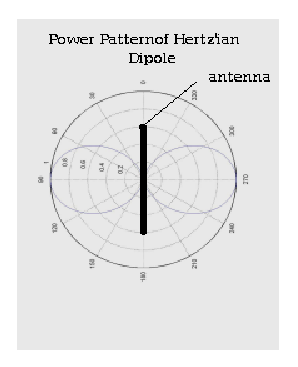
\includegraphics[width=8cm]{pp_hd}\\
  \caption{Power pattern of Hertzian Dipole}\label{fig_pp_hd}
\end{center}
\end{figure}


\paragraph*{}
Figure (\ref{fig_pp_hd}) shows the power pattern of a Hertzian Dipole as function of the colatitude. When treating the reception qualities of an antenna, it is possible to define an effective antenna area $\Sigma_{eff}$, such that the received power is just the incoming power flux multiplied by this area.

\begin{equation}\label{effect_area}
\Sigma_{eff}(\theta,\phi)=\frac{\lambda^2}{4\pi}G(\theta,\phi)
\end{equation}

\paragraph*{}
The effective area depends on the direction of the incoming wave. Of course, it has nothing to do with the geometric size of the antenna.

\paragraph*{}
Now some real antennas are treated, building upon the knowledge of this section.
\newpage
\section{\textbf{Real antennas and their properties}}

\paragraph*{}\index{Cassini}
The simplest, real antenna is the short dipole. A short dipole has a length that is small in relation to the wavelength, but not infinitesimal. This sort of antenna is often used in spacecraft like CASSINI, for radio science experiments. The lengths of the antennas vary between a few meters to 12-15 meters and are used to receive radiation with a wavelength in the order of a few hundred meters. The current distribution along the antenna is now not constant along the antenna, but

\begin{equation}\label{shd_current}
 \mathbf{j} = \mathbf{\hat{z}} I(z') \delta (x') \delta (y')
\end{equation}

\paragraph*{}
is all, one can say about its form without further information. Since the dipole is short in relation to the wavelength, we can, at least, say that the phase is the same at any point of the antenna. This simplifies the situation to some extent. Putting (\ref{shd_current}) in (\ref{fraunhofer_A}), one gets the vector potential:
\index{Fraunhofer approximation}

\begin{equation}\label{shd_A}
 \mathbf{A}_{ff}(\mathbf{r},t) = \mathbf{\hat{z} }\frac{\mu_0}{4 \pi r} e^{-ikr} \int_{-\frac{l}{2}}^{\frac{l}{2}} I(z') e^{ik z'\cos \theta } dz'
\end{equation}

\paragraph*{}
and due to the constant phase, this simplifies to

\begin{equation}\label{shd_A_simpl}
\mathbf{A}_{ff}(\mathbf{r},t) = \mathbf{\hat{z}} \frac{\mu_0}{4 \pi r} e^{-ikr} \int_{-\frac{l}{2}}^{\frac{l}{2}} I(z') dz'
\end{equation}

\paragraph*{}
One can define an effective antenna length $l_{eff}$ in a way that

\begin{equation}\label{defin_leff}
Il_{eff}= \int_{-\frac{l}{2}}^{\frac{l}{2}} I(z') dz'
\end{equation}

\paragraph*{}
and so circumvents the problem that the actual current distribution is unknown. Then

\begin{equation}\label{shd_A_solution}
\mathbf{A}_{ff}(\mathbf{r},t) = \mathbf{\hat{z}} \frac{\mu_0 I l_{eff}}{4 \pi r} e^{-ikr}
\end{equation}

\paragraph*{}
If the current was constant along the wire, like in the Hertzian Dipole, the effective length would have the same magnitude than the physical length. But, as said before, this is not possible in reality. It is difficult to determine the actual current distribution, the only thing that can be said for sure is, that the current must be zero at all times at the tips of the antenna. For many purposes a linear current distribution, which is the easiest to deal with, is good enough. In this case, according to equation (\ref{defin_leff}), we can calculate the effective length.
\index{current distribution}

%\begin{figure}
%  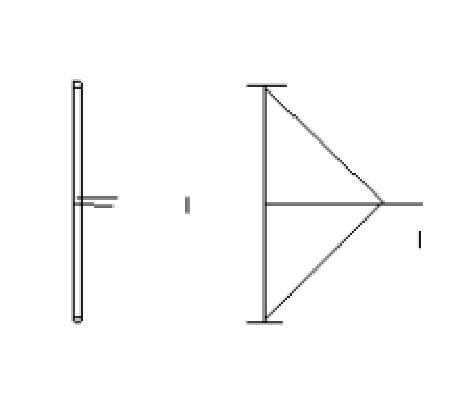
\includegraphics[width=12cm]{curr_distr_shd}\\
%  \caption{Linear current distribution}\label{fig_curr_distr_shd}
%\end{figure}

\begin{eqnarray}
I&=&I_0 \left( \frac{\frac{l}{2}-|z'|}{\frac{l}{2}}\right) \label{l_eff_shd_1} \\
\Rightarrow  l_{eff}&=& \frac{1}{I} \int_{-\frac{l}{2}}^{\frac{l}{2}} I_0 \left( \frac{\frac{l}{2}-|z'|}{\frac{l}{2}}\right) dz' \label{l_eff_shd_2} \\
&=&\frac{l}{2} \nonumber
\end{eqnarray}

\paragraph*{}
The physical fields can be calculated in the same way as for the Hertzian Dipole, one has just to use the effective dipole length instead of the geometric length. Gain, Directivity and power pattern are the same as for the Hertzian Dipole, since they are independent of antenna length. The resistivity is $\approx 20 (k l_{eff} )^2$
\index{dipole!short}
\paragraph*{}
Another type of antenna is the monopole. It can be seen as a dipole, where the ground plane has the function of the second branch. The actual configurations of the fields can be calculated by using the method of mirror charges, so a monopole over a ground plane emits the same way as a short dipole. A spacecraft with a monopole can be modeled in a way such that the spacecraft hull takes the role of the second branch. Of course, the radiation pattern will be altered in this case. Not only the effective length of the antenna will be altered, but also the direction. One speaks of the effective length vector, which is, in general, complex and dependent upon frequency and direction of the radiation.

\paragraph*{}\index{dipole!halfwave}
The Halfwave Dipole has a length that is exactly half of the wavelength of the emitted wave. The propagation delays between signals that are produced in different parts of the wire have to be taken into account. The current can be approximated by

\begin{equation}\label{hwd_current}
 \mathbf{I}(z') = \mathbf{\hat{z}} I_0 \cos kz'
\end{equation}

\begin{figure}
  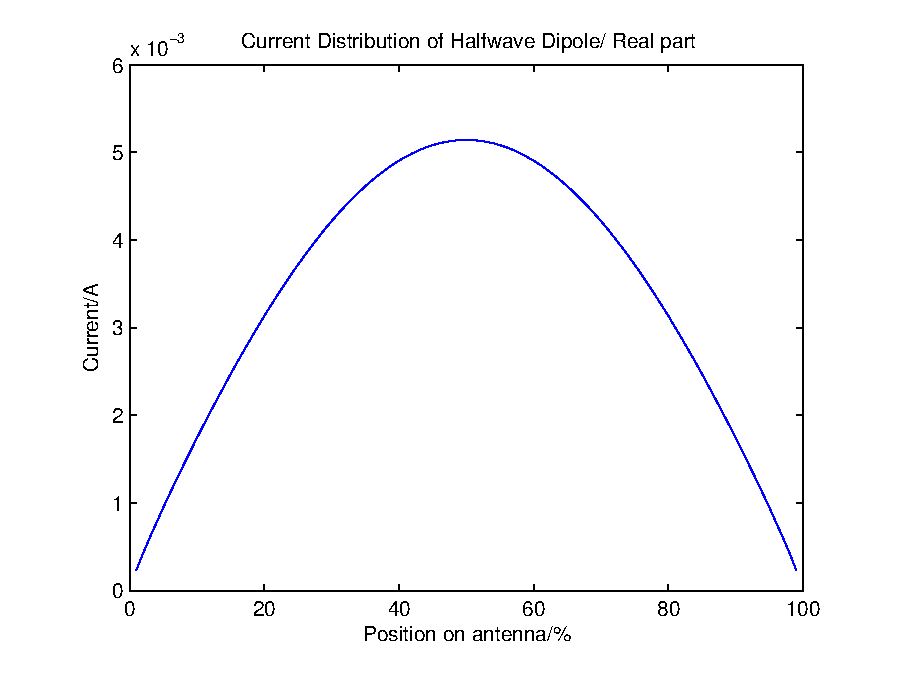
\includegraphics[width=12cm]{phase_distr_shd}\\
  \caption{Current distribution of the Halfwave Dipole}\label{fig_curr_distr_hwd}
\end{figure}

\paragraph*{}\index{vector potential}
The vector potential can be calculated by using (\ref{fraunhofer_A}).

\begin{eqnarray}\label{hwd_A_solution}
 \mathbf{A}_{ff}(\mathbf{r},t) &=&\mathbf{ \hat{z}} \frac{\mu_0}{4 \pi r} e^{-ikr} \int_{-\frac{\lambda}{4}}^{\frac{\lambda}{4}} I_0 \cos kz' e^{ikz'\cos \theta } dz'\\
&=& \mathbf{\hat{z}} \frac{\mu_0}{4 \pi r} e^{-ikr} \int_{-\frac{\lambda}{4}}^{\frac{\lambda}{4}} \frac{1}{2} I_0 (e^{-ikz'}+e^{ikz'}) e^{ikz'\cos \theta } dz'\nonumber \\
&=& \mathbf{\hat{z} }\frac{\mu_0 I_0}{4 \pi r} e^{-ikr} \left[ \frac{e^{-ikz' (1+ \cos \theta ) }}{2ik(1+ \cos \theta )} + \frac{e^{-ikz' (-1+ \cos \theta )} }{2ik(-1+ \cos \theta )} \right]_{-\frac{\lambda}{4}}^{\frac{\lambda}{4}} \nonumber \\
&=& \mathbf{\hat{z}} \frac{\mu_0 I_0}{4 \pi r} e^{-ikr} \frac{\cos (\frac{\pi}{2} \cos \theta)}{\sin^2 \theta} \nonumber
\end{eqnarray}

\paragraph*{}
The fields can be derived with equations (\ref{rule_Hff}) and (\ref{rule_Eff}), using the geometrical identity, that $\mathbf{\hat{r}} \times \mathbf{\hat{z}}=- \mathbf{\hat{\phi}} \sin \theta$.

\begin{eqnarray}
\mathbf{H}_{ff} (\mathbf{k},\omega)&=&  - \frac{1}{\mu_0} ik\mathbf{\hat{r}} \times \mathbf{A}_{ff} \label{hwd_Hff} \\
&=& -(\mathbf{\hat{r} }\times\mathbf{ \hat{z}})  \frac{ik I_0}{4 \pi r} e^{-ikr} \frac{\cos (\frac{\pi}{2} \cos \theta)}{\sin^2 \theta}\nonumber \\
&=& \mathbf{\hat{\phi}}  \frac{ik I_0}{4 \pi r} e^{-ikr} \frac{\cos (\frac{\pi}{2} \cos \theta)}{\sin \theta} \nonumber \\
\mathbf{E}_{ff} (\mathbf{k},\omega)&=&  i \omega \mathbf{\hat{r}} \times ( \mathbf{\hat{r}} \times \mathbf{A}_{ff}) \label{hwd_Eff} \\
&=& \mathbf{\hat{\theta}} \frac{i \eta_0 k I_0}{2 \pi r} e^{-ikr} \frac{\cos (\frac{\pi}{2} \cos \theta)}{\sin \theta} \nonumber
\end{eqnarray}

\paragraph*{}\index{L'H\^{o}pital's rule}
To take care of the singularity at the poles of the antenna ($\theta=0$), one can use L'H\^{o}pital's rule, so the vector potential and the fields are zero, when theta is zero. Total power that is radiated by the Halfwave Dipole, is

\begin{eqnarray}\label{total_power_hwd}
P_{rad} &=& \int_0^{2\pi } \partial \phi \int_0^{\pi} r^2 \sin \theta \frac{1}{2 \eta_0} \left( \frac{\eta_0 I_0}{2 \pi r} \right)^2  \frac{\cos^2 (\frac{\pi}{2} \cos \theta)}{\sin^2 \theta} \partial \theta  \\
&=& \frac{\eta_0}{4 \pi} I_0^2 \int_0^{\pi} \frac{\cos^2 (\frac{\pi}{2} \cos \theta)}{\sin^2 \theta} \partial \theta \nonumber \\
&\approx& 36.5 I_0^2 \nonumber
\end{eqnarray}

\paragraph*{}
The integral over theta has to be evaluated numerically. The radiation resistance is
\index{radiation resistance}
\begin{equation}\label{radiation_resistance_hwd}
R_{rad} = \frac{2 P_{rad}}{I_0^2}=73 \Omega
\end{equation}

\paragraph*{}
which is good news in terms of impedance matching. For the computation of the Gain, one best uses equation (\ref{gain})
\index{impedance matching}
\begin{equation}\label{gain_hwd}
G( \theta , \phi )= 1.64 \frac{\cos^2 (\frac{\pi}{2} \cos \theta)}{\sin^2 \theta}
\end{equation}

\paragraph*{}
when the antenna is impedance matched, i.e. there are no losses due to reflections. The maximum Gain is slightly higher than that of the Hertzian Dipole. This means, the directivity of the antenna is higher, as one can see, when observing the power pattern as in figure \ref{fig_pp_shd}.

\begin{figure}
 \begin{center}
 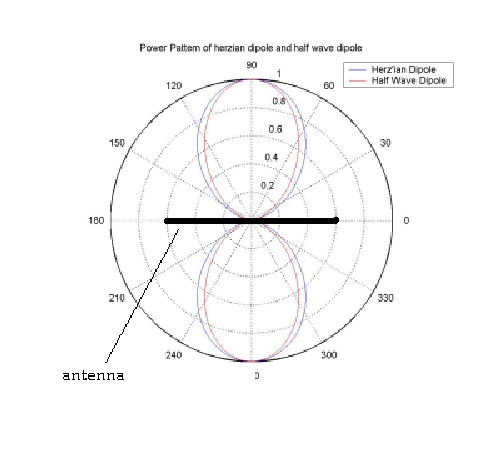
\includegraphics[width=8cm]{pp_shd}\\
  \caption{Power Pattern of the Halfwave Dipole}\label{fig_pp_shd}
  \end{center}
\end{figure}

\begin{figure}
  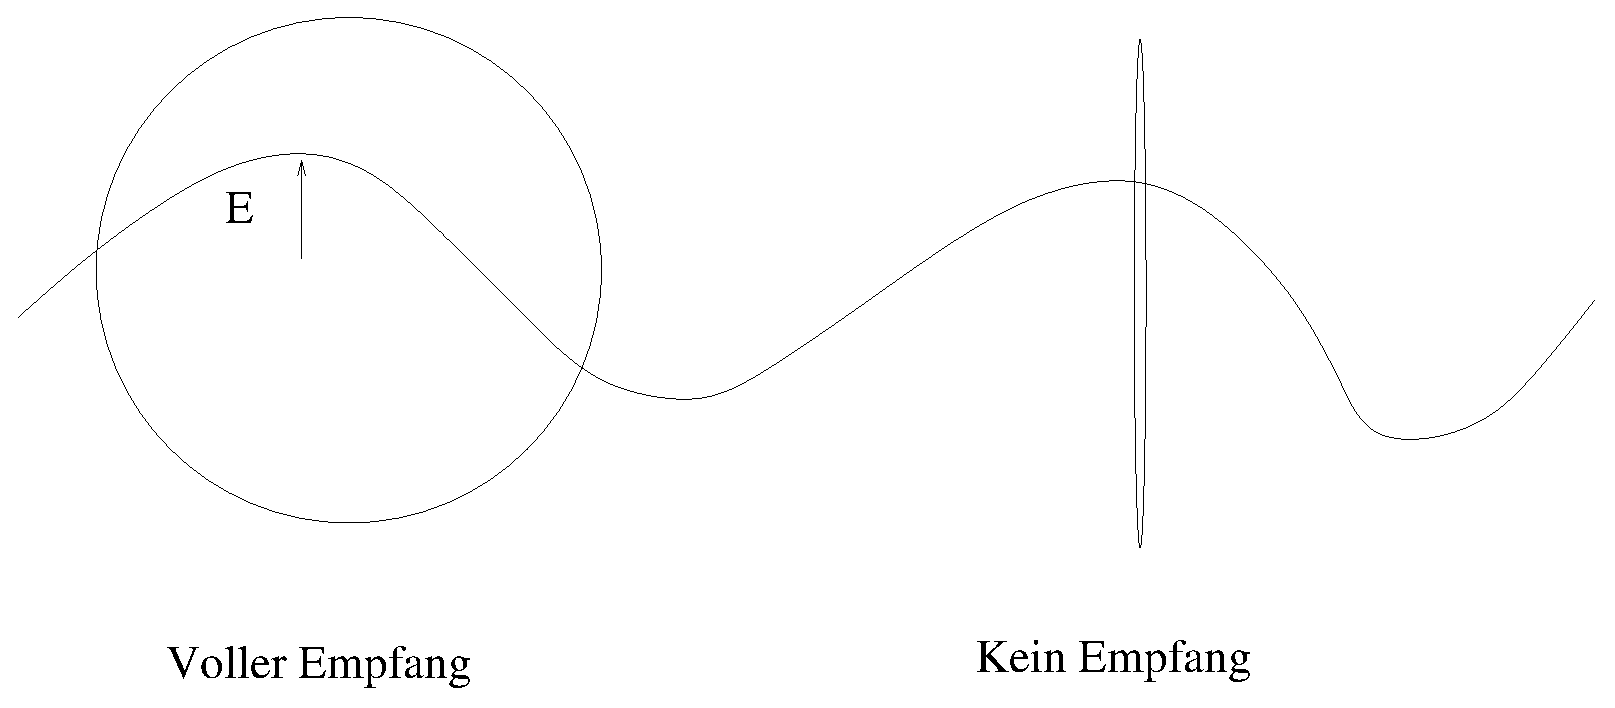
\includegraphics[width=12cm]{loop.eps}\\
  \caption{Loop antenna}\label{fig_loop}
\end{figure}
\paragraph*{}\index{antenna!loop}
Small loop antennas were the first antennas used for direction finding, back in the twenties of the last century (Fig. \ref{fig_loop}). To get an insight into their characteristics, we can calculate their vector potential. Since the situation is obviously rotational symmetric, we can arbitrarily use $\varphi=0$.

\begin{eqnarray}\label{A_loop}
 \mathbf{A}_{ff}(\mathbf{r},t) &=& \frac{\mu_0}{4 \pi r} e^{-ikr} \int_{V'} \mathbf{j}(\mathbf{r}') e^{ik \mathbf{\hat{r}} \cdot \mathbf{r}' } dV' \\
&=& \frac{\mu_0}{4 \pi r} e^{-ikr} \int_{0}^{2\pi}\mathbf{ \hat{\varphi}'} I e^{ik \mathbf{\hat{r}} \cdot \mathbf{r}' } a d\varphi' \nonumber \\
&=& \frac{\mu_0 I a}{4 \pi r} e^{-ikr} \int_{0}^{2\pi} (-\mathbf{\hat{x}}\sin \varphi ' + \mathbf{\hat{y}} \cos \varphi ') e^{ik a\sin \theta \cos \varphi' }  d\varphi' \nonumber
\end{eqnarray}

\paragraph*{}
a is the radius of the loop. When the radius of the loop is small in relation to the wavelength ($ka\ll 1$), we can approximate the exponential term under the integral by its Taylor polynom of rank one.

\begin{equation}\label{taylor}
e^{ik a\sin \theta \cos \varphi' } \rightarrow 1+ik a\sin \theta \cos \varphi'
\end{equation}

\paragraph*{}
Hence
\begin{eqnarray}\label{A_loop_2}
 \mathbf{A}_{ff}(\mathbf{r},t) &=& \frac{\mu_0 I a}{4 \pi r} e^{-ikr} \int_{0}^{2\pi} (-\mathbf{\hat{x}}\sin \varphi ' + \mathbf{\hat{y}} \cos \varphi ') (1+ik a\sin \theta \cos \varphi')   d\varphi' \nonumber \\
&=& \frac{\mu_0 I a}{4 \pi r} e^{-ikr} \{ - \mathbf{\hat{x}} \int_{0}^{2\pi} \sin \varphi ' d\varphi' +  \mathbf{\hat{y}} \int_{0}^{2\pi}  \cos \varphi ' d\varphi' \nonumber \\
&+&  ik a \sin \theta \mathbf{\hat{x}} \int_{0}^{2\pi}  \cos \varphi' \sin \varphi ' d\varphi'+  ik a\sin \theta  \mathbf{\hat{y}} \int_{0}^{2\pi}\cos^2 \varphi'  d\varphi' \} \nonumber \\
&=& \frac{\mu_0 I a}{4 \pi r} e^{-ikr} \{ 0 +  0 \nonumber \\
&+&  0 +  ik a \sin \theta \mathbf{\hat{y}} \left[ \frac{1}{2} \left( \varphi' +\frac{1}{2} sin(2\varphi') \right) \right]_{0}^{2\pi} \} \nonumber \\
&=& \mathbf{\hat{y}} \frac{i \mu_0 k I \pi a^2}{4 \pi r} e^{-ikr} \sin \theta  \nonumber \\
\end{eqnarray}

\paragraph*{}
But when $\varphi = 0$, the y-direction is equal to the $\varphi$ direction, so

\begin{eqnarray}\label{A_loop_2}
 \mathbf{A}_{ff}(\mathbf{r},t)|_{\varphi=0} &=& \mathbf{\hat{\varphi} }\frac{i \mu_0 k I \pi a^2}{4 \pi r} e^{-ikr} \sin \theta  \nonumber \\
\end{eqnarray}

\paragraph*{}
The fields can be calculated as before:

\begin{eqnarray}
\mathbf{H}_{ff} (\mathbf{r},t)&=& - \frac{1}{\mu_0} ik\mathbf{\hat{r}} \times \mathbf{A}_{ff} \label{Hff_loop}\\
&=& - \mathbf{\hat{\theta}} \frac{k^2 I \pi a^2}{4 \pi r} e^{-ikr} \sin \theta \nonumber
\end{eqnarray}

\begin{eqnarray}
\mathbf{E}_{ff} (\mathbf{r},t)&=& i \omega \mathbf{\hat{r}} \times ( \mathbf{\hat{r}} \times \mathbf{A}_{ff}) \label{Eff_loop} \\
&=& \mathbf{\hat{\varphi}} \frac{\eta_0 k^2 I \pi a^2}{4 \pi r} e^{-ikr} \sin \theta \nonumber
\end{eqnarray}


\paragraph*{}\index{antenna!gain}
When comparing the equations of the fields with those of the dipole, it is easy to see that they have exactly the same shape. They just differ in magnitude and the magnetic and electric fields are exchanged. Therefore, a loop is said to be dual to a dipole. Often, it is called \emph{magnetic dipole}. The Gain is exactly the same as in the case of the Hertz'ian Dipole and the radiated power is:

\begin{eqnarray}\label{total_power_loop}
P_{rad}&=& \int_0^{2\pi } \partial \phi \int_0^{\pi} r^2 \sin \theta \frac{1}{2 \eta_0} \left[ \frac{\eta_0 k^2 I \pi a^2}{4 \pi r} \right]^2 \sin^2 \theta \partial \theta  \\
&=& \frac{\pi}{12} \eta_0 (ka)^4 I^2 \nonumber
\end{eqnarray}\index{radiated power}

\paragraph*{}\index{radiation resistance}
and the radiation resistance is

\begin{eqnarray}\label{radiation_resistance_loop}
R_{rad} &=& \frac{2 P_{rad}}{I^2} \\
&=&  \frac{\pi}{12} \eta_0 (ka)^4 \nonumber \\
&\approx& 3.1 \cdot 10^5  \left(\frac{a}{\lambda} \right)^4 \Omega \nonumber
\end{eqnarray}

\paragraph*{}
A coil with N loops behaves like the sum of N loops. Hence, to calculate the behavior of a coil the substitution\index{coil}

\begin{equation}\label{coil_subst}
I\rightarrow NI
\end{equation}


\paragraph*{}
can be performed. The Gain remains the same, since it is independent of the current and the other important observables have the following equations :

\begin{eqnarray}
P_{rad} &=&N^2 P_{rad,loop} \\
R_{rad} &\approx& 3.1 \cdot 10^5  N^2 \left(\frac{a}{\lambda} \right)^4 \Omega
\end{eqnarray}

\paragraph*{}
A coil has a more compact geometry than a dipole and it is easier to produce a large radiation power and, as a result, also a good receiving sensitivity with it than with a dipole.

\section{\textbf{Phased arrays}}
\paragraph*{}\index{phased array}
When using more than one antenna, one can modify and model the direction and directivity of the beam, by controlling the amplitude and relative phase of each antenna, also called element in this context. The resultant beam is built by the laws of interference. The more antennas, the sharper the beam can be modeled. Active beam steering, which is the control of the beam without physically moving any parts of the antenna, can be done two or three dimensional, depending on whether one has a one- or two dimensional antenna array.\index{active beam steering}

\paragraph*{}
Thanks to the linearity of Maxwell's equations it is easy to calculate the potential or physical fields of an array, once one has the fields of the single components. One has just to add them. If there is, for example, an array of N short dipoles, all directed along the z-axis, the electric field is

\begin{equation}\label{Eff_array}
\mathbf{E} = \sum_{i=1}^N\mathbf{ \hat{\theta} }\frac{i \eta_0 k I_i l_{eff,i}}{4 \pi r_i} e^{-ikr_i } \sin \theta_i
\end{equation}

\paragraph*{}
The same procedure is possible for all other fields and antennas. If the spatial distribution of the elements is small in relation to the distance of the observer (Fraunhofer approximation) and all elements are of the same kind and orientation, the equation can be further simplified. The distance of the observer from an element i is $r_i=|\mathbf{r}-\mathbf{a_i}|\approx r-\mathbf{\hat{r}} \cdot \mathbf{a_i} $. The angle $\theta$ is approximately equal for all elements, so $\theta_i \rightarrow \theta$ and $1/r_i$ can safely be replaced by $1/r$. But is is not reasonable to believe that $ka_i$ is small, so there must be included a phase factor that describes the difference in phase for each element. And the difference in amplitude has also to be taken into account, which can be done by defining a complex weight factor for each element: $w_i=I_il_{eff,i}/Il_{eff}$. Putting everything together, we can write

\begin{equation}\label{Eff_array_simpli}
\mathbf{E} = \left[ \mathbf{\hat{\theta}} \frac{i \eta_0 k I l_{eff}}{4 \pi r} e^{-ikr } \sin \theta \right] \left[ \sum_{i=1}^N w_i e^{ik \mathbf{\hat{r}} \cdot \mathbf{a_i}} \right]
\end{equation}

\paragraph*{}
The first part of the right hand side of the equation bears information about the elements of the array, the second part describes the phase and amplitude difference between the elements. Defining an element factor $\mathfrak{E}$ and a phase factor $\mathfrak{P}$ to write (\ref{Eff_array_simpli}) in condensed form:

\begin{equation}\label{Eff_array_simpli_simpli}
\mathbf{E} = \mathfrak{E}\mathfrak{P}
\end{equation}

\paragraph*{}
A similar procedure can be done with the other fields. However, due to the fact that, as I mentioned before, up to now the concept of phased arrays not used in spacecraft, the treatment of this subject is stopped at this point. In other areas, phased arrays are used to a great extent.

\section{\textbf{The reciprocity theorem}}

\paragraph*{}\index{reciprocity theorem}
The reciprocity theorem is a highly complicated matter, which will not be dealed with in depth here. However, it is worthwhile to present some interesting conclusions which are of direct importance in space science.

\paragraph*{}
If two sources of EM radiation exist, say A and B, then the medium in which they are embedded is called reciprocal if the following relations are true:\index{media!reciprocal}

\begin{eqnarray}
\mathbf{B}_B \cdot \mathbf{H}_A &=& \mathbf{B}_A \cdot \mathbf{H}_B \label{reciproci_1} \\
\mathbf{D}_B \cdot \mathbf{E}_A &=& \mathbf{D}_A \cdot \mathbf{E}_B \label{reciproci_2}
\end{eqnarray}

\paragraph*{}
From a technical viewpoint, this means that the receiving properties are equal to the emitting properties of a given antenna. This is always true in vacuum. When tensor notation has to be used, equations (\ref{reciproci_1}) and (\ref{reciproci_2}) are true if the following relations hold:

\begin{eqnarray}
\mathbf{\mu} &=& \mathbf{\mu}^T \label{reciproci_tensor_1} \\
\mathbf{\varepsilon} &=& \mathbf{\varepsilon}^T \label{reciproci_tensor_2}
\end{eqnarray}

\paragraph*{}\index{reciproci tensor}
This is not the case for magnetized plasma, so space plasma is, in principle a medium where the reciprocity theorem is not valid.

\chapter{\textbf{Direction Finding}}
\section{\textbf{DF Basics}}
\paragraph*{}\index{direction finding}
Direction finding (DF) can be defined as the procedure to find the direction and the polarization of the incident wave by using the measured data. Figure \ref{fig_coordinate_frame_DF} defines the symbols and coordinate system which will be used throughout this section (for detailed description see also
\cite{ladreiter_03}).\\

\begin{figure}
  % Requires \usepackage{graphicx}
  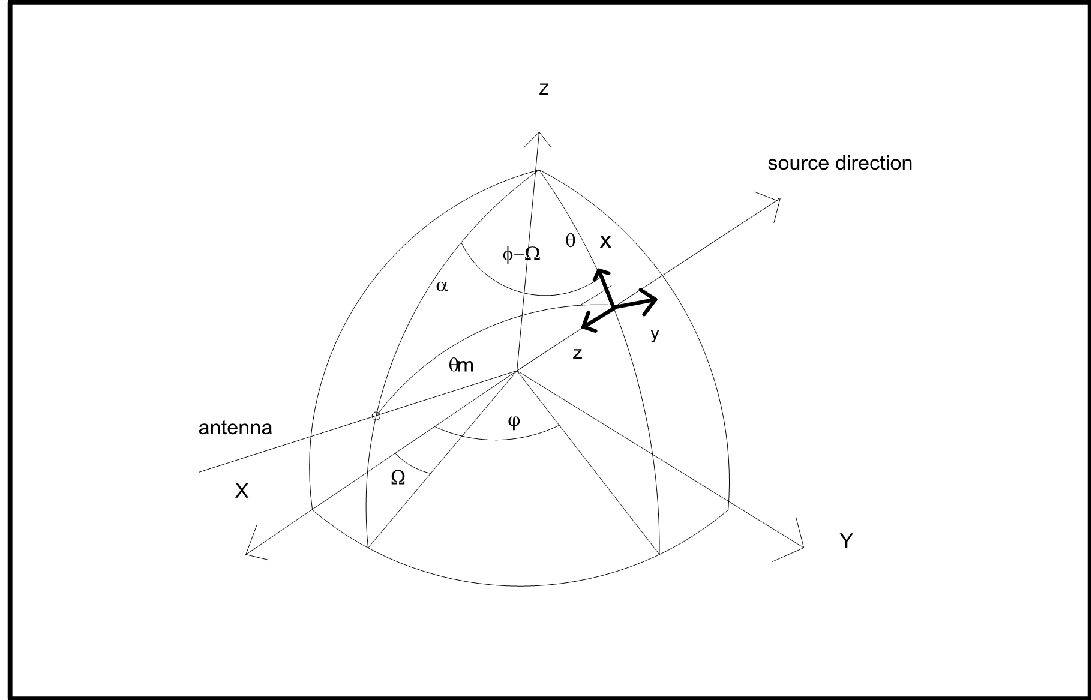
\includegraphics[width=12cm]{df_coordinate_system.eps}\\
  \caption{Coordinate frame}\label{fig_coordinate_frame_DF}
\end{figure}

\paragraph*{}
X, Y and Z define the spacecraft centered orthogonal cartesian coordinate system, while x,y and z define the coordinate system of the incident electromagnetic wave. The wave vector $\textbf{k}$ points in the positive z-axis, so the equation of the electric field of the wave is
\begin{equation}
\textbf{E}=\textbf{E}_0 e^{i(\textbf{k} \cdot \textbf{r} - \omega t)}
\end{equation}

\paragraph*{}
The electric field is the sum of the components in x and y direction. There is no component in the z direction.
\begin{eqnarray}
\textbf{E}&=&E_x\textbf{e}_x + E_y\textbf{e}_y\\
E_x&=&E_{0,x} e^{i(kz - \omega t)} \label{Ex} \\
E_y&=&E_{0,y} e^{i(kz - \omega t - \delta)} \label{Ey}
\end{eqnarray}
\paragraph*{}
$\delta$ is the phase shift between the x and y components of the E-field. The direction of the incident wave is defined by the angles $\vartheta$ and $\varphi$, the effective height vector points to the direction that is defined by the angles $\alpha$ and $\Omega$.
\paragraph*{}
The 4 Stokes parameter define the polarization of the wave. They can be written in the following form:
\begin{equation}
S_0=I= \left\langle E_{x}^2\right\rangle +\left\langle E_{y}^2\right\rangle
\end{equation}
\begin{equation}
S_1=Q=\left\langle E_{x}^2\right\rangle-\left\langle E_{y}^2\right\rangle
\end{equation}
\begin{equation}
S_2=U=\left\langle2E_{x} E_{y} \cos \delta \right\rangle
\end{equation}
\begin{equation}
S_3=V=\left\langle2E_{x} E_{y} \sin\delta\right\rangle
\end{equation}
\\
\paragraph*{}\index{Stokes parameter}
The Stokes Parameters are more useful in normalized form.
\begin{eqnarray}
\frac{S_0}{2\eta_0} = \hat{I} &=& \frac{\left\langle E_{x}^2\right\rangle +\left\langle E_{y}^2\right\rangle}{2\eta_0} \label{norm_stokes_1}
\\
\frac{S_1}{S_0}=\hat{Q}&=&\frac{\left\langle E_{x}^2\right\rangle-\left\langle E_{y}^2\right\rangle}{\left\langle E_{x}^2\right\rangle +\left\langle E_{y}^2\right\rangle}\label{norm_stokes_2}
\\
\frac{S_2}{S_0}=\hat{U}&=&\frac{\left\langle2E_{x} E_{y} \cos\delta\right\rangle}{\left\langle E_{x}^2\right\rangle +\left\langle E_{y}^2\right\rangle}\label{norm_stokes_3}
\\
\frac{S_3}{S_0}=\hat{V}&=&\frac{\left\langle2E_{x} E_{y} \sin\delta\right\rangle}{\left\langle E_{x}^2\right\rangle +\left\langle E_{y}^2\right\rangle}\label{norm_stokes_4}
\end{eqnarray}
\paragraph*{}\index{autocorrelation parameter}\index{crosscorrelation parameter}
The output values of the measurements are the auto- and crosscorrelation parameters. For two antennas X and Z, they would be\\
\\
\begin{center}
\begin{tabular}{c}
$\left\langle V_X V_X^* \right\rangle $  \\
$\left\langle V_Z V_Z^* \right\rangle $  \\
$Re\left\langle V_X V_Z^* \right\rangle $  \\
$Im\left\langle V_X V_Z^* \right\rangle $  \\
\end{tabular}
\end{center}

\paragraph*{}
$V_i$ is the voltage induced in antenna i and the star means the complex conjugate. The angular brackets indicate the mean value. In general, for a complex function $C(t)$,
\begin{equation}
\left\langle CC^* \right\rangle = \frac{1}{T}\int_0^T CC^* dt
\end{equation}

\paragraph*{}
This equation gives only a good result, if T is large in relation to the period of the EM wave. So the next step is to find a formula for V. The basic equation, upon which the method of direction finding is built, is
\begin{equation}
V=\textbf{h}_{eff}\cdot \textbf{E}
\end{equation}
\paragraph*{}
$\textbf{h}_{eff}$ is the effective length vector. The radiation pattern of the antenna looks like a sole monopole which points in the direction of $\textbf{h}_{eff}$ and with the length of the vector magnitude. In general, the effective length vector depends on the frequency and direction of the incoming wave. These dependencies can be neglected for low frequencies. At wavelengths that are large in relation to the receiving antenna, $h_{eff}$ can be expected to be approximately half of the physical antenna.
\paragraph*{}
When written in component form, one can write
\begin{equation}
V=h_{eff,x} E_x + h_{eff,y} E_y \footnote{The coordinate frame is defined in a way that the electric field has no z-component.}
\end{equation}
\paragraph*{}
After substituting equations (\ref{Ex}) and (\ref{Ey}) one obtains
\begin{equation}
V=h_{eff,x} E_{0,x} e^{i(kz - \omega t)}  + h_{eff,y} E_{0,y} e^{i(kz - \omega t - \delta)}
\end{equation}
\paragraph*{}
If the antenna is located at z=0 and short in relation to the wavelength, it can be simplified.
\begin{equation}
V=h_{eff,x} E_{0,x} e^{i(\omega t)}  + h_{eff,y} E_{0,y} e^{i(\omega t - \delta)}\label{V}
\end{equation}
\paragraph*{}
Hence, the next step is to find the x and y components of $\textbf{h}_{eff}$. By using the unit vector in the direction of $\textbf{h}_{eff}$, one can write

\begin{equation}
\textbf{h}_{eff} = h_{eff}\left[ \begin{array}{c}
\sin \alpha \cos \Omega\\
\sin \alpha \sin \Omega\\
\cos \alpha
\end{array}  \right]
\end{equation}

\paragraph*{}
The unit vectors of the spherical coordinate system are
\begin{eqnarray}
\textbf{e}_r &=& \left[ \begin{array}{c}
\sin \theta \cos \varphi\\
\sin \theta \sin \varphi\\
\cos \theta
\end{array}  \right] \\
\textbf{e}_\theta &=& \left[ \begin{array}{c}
\cos \theta \cos \varphi\\
\cos \theta \sin \varphi\\
-\sin \theta
\end{array}  \right] \\
\textbf{e}_\varphi &=& \left[ \begin{array}{c}
-\sin  \varphi\\
\cos \varphi\\
0
\end{array}  \right]
\end{eqnarray}
\paragraph*{}
By looking at Figure \ref{fig_coordinate_frame_DF}, one can easily see that the direction of the negative x-axis (small x) is also the negative $\theta$ direction  $(\textbf{e}_x=-\textbf{e}_\theta)$. Hence

\begin{equation}
{h}_{eff,x} = -h_{eff} \left[ \begin{array}{c}
\sin \alpha \cos \Omega\\
\sin \alpha \sin \Omega\\
\cos \alpha
\end{array}  \right] \cdot \left[ \begin{array}{c}
\cos \theta \cos \varphi\\
\cos \theta \sin \varphi\\
-\sin \theta
\end{array}  \right]
\end{equation}
\paragraph*{}
That is
\begin{equation}
{h}_{eff,x} = h_{eff}( \sin \theta \cos \alpha - \sin \alpha \cos\theta\cos (\varphi - \Omega ) )\label{heff_x}
\end{equation}
\paragraph*{}
Equivalently $\textbf{e}_y=\textbf{e}_\varphi$.
\begin{equation}
{h}_{eff,y} = h_{eff} \left[ \begin{array}{c}
\sin \alpha \cos \Omega\\
\sin \alpha \sin \Omega\\
\cos \alpha
\end{array}  \right] \cdot \left[ \begin{array}{c}
-\sin \varphi\\
\cos \varphi\\
0
\end{array}  \right]
\end{equation}
\paragraph*{}
or
\begin{equation}
{h}_{eff,y} = -h_{eff}( \sin \alpha \sin (\varphi - \Omega ) )\label{heff_y}
\end{equation}

\paragraph*{}
Using equations (\ref{V}), (\ref{heff_x}) and (\ref{heff_y}), one can get a general expression for the voltage which is induced in an antenna.
\begin{eqnarray}
V & = & h_{eff} [ (\sin \theta \cos \alpha - \sin \alpha \cos \theta \cos (\varphi - \Omega) )E_{0,x}e^{i \omega t} - \nonumber \\
& & -(\sin \alpha \sin (\varphi - \Omega))E_{0,y}e^{i (\omega t-\delta) } ] \nonumber \\
& = & h_{eff} e^{i \omega t} [ (\sin \theta \cos \alpha - \sin \alpha \cos \theta \cos (\varphi - \Omega) )E_{0,x} - \\
& & -(\sin \alpha \sin (\varphi - \Omega))E_{0,y}e^{-i \delta } ] \nonumber
\end{eqnarray}

\paragraph*{}
This equation is valid for any monopole antenna, irrespective of its orientation as long as the frequency is low enough, such that the imaginary parts of the effective length vectors are vanishing small. To model the observables, one has to perform the necessary multiplications. For two antennas, indexed i and j, one gets

\begin{eqnarray}
V_i V_i^{*} &=& h_{eff,i}^2[E_{0,x}^2 (\sin^2 \theta \cos^2 \alpha_i -\frac{1}{2} \sin (2\alpha_i) \sin(2\theta) \cos^2(\varphi - \Omega_i) + \nonumber \\
& & + \sin^2\alpha_i \cos^2\theta \cos^2(\varphi - \Omega_i))+ \\
& & + E_{0,y}^2 \sin^2\alpha_i \sin^2 (\varphi - \Omega_i) +\nonumber \\
& & +  \frac{1}{2} E_{0,x} E_{0,y} (-\sin \theta \sin 2\alpha_i \sin(\varphi - \Omega_i) + \nonumber \\
&&+\sin^2\alpha_i \cos \theta sin(2\varphi - 2\Omega_i)) (e^{i \delta} + e^{-i \delta } )]\nonumber
\end{eqnarray}
and
\begin{eqnarray}
V_i V_j^{*} &=& h_{eff,i} h_{eff,j}[E_{0,x}^2 (\sin^2 \theta \cos \alpha_i \cos \alpha_j - \\
& & - \frac{1}{2}  \sin(2\theta) (\sin \alpha_j \cos \alpha_i \cos(\varphi - \Omega_j)+ \nonumber \\
& & +\sin \alpha_i \cos \alpha_j \cos(\varphi - \Omega_i) )+ \nonumber \\
& & + \sin \alpha_i \sin \alpha_j \cos^2\theta \cos(\varphi - \Omega_i) \cos(\varphi - \Omega_j))+ \nonumber \\
& & + E_{0,y}^2 \sin \alpha_i \sin \alpha_j \sin (\varphi - \Omega_i) \sin (\varphi - \Omega_j)\nonumber \\
& & -E_{0,x} E_{0,y} e^{i \delta}( \sin \alpha_j \sin(\varphi - \Omega_j)( \cos \alpha_i \sin \theta - \nonumber \\
& &- \sin \alpha_i \cos \theta \cos(\varphi - \Omega_i)))-\nonumber \\
& &  -E_{0,x} E_{0,y} e^{-i \delta}( \sin \alpha_i \sin(\varphi - \Omega_i)( \cos \alpha_j \sin \theta - \nonumber \\
& & -\sin \alpha_j \cos \theta \cos(\varphi - \Omega_j)))]\nonumber
\end{eqnarray}

\paragraph*{}
When standardized over time

\begin{eqnarray}
\left\langle V_i V_i^{*} \right\rangle &=&  h_{eff,i}^2[\left\langle E_{0,x}^2\right\rangle (\sin^2 \theta \cos^2 \alpha_i -\nonumber\\
& & -\frac{1}{2} \sin (2\alpha_i) \sin(2\theta) \cos^2(\varphi - \Omega_i) + \\
& & + \sin^2\alpha_i \cos^2\theta \cos^2(\varphi - \Omega_i))+ \nonumber \\
& & + \left\langle E_{0,y}^2 \right\rangle \sin^2\alpha_i \sin^2 (\varphi - \Omega_i)+ \nonumber \\
& & +  \left\langle E_{0,x} E_{0,y} \cos \delta \right\rangle (-\sin \theta \sin 2\alpha_i \sin(\varphi - \Omega_i) + \nonumber \\
& &+ \sin^2\alpha_i \cos \theta sin(2\varphi - 2\Omega_i)) ]\nonumber
\end{eqnarray}

\begin{eqnarray}
Re \left\langle V_i V_j^{*}\right\rangle &=&  h_{eff,i} h_{eff,j}[\left\langle E_{0,x}^2\right\rangle (\sin^2 \theta \cos \alpha_i \cos \alpha_j - \\
& & - \frac{1}{2}  \sin(2\theta) (\sin \alpha_j \cos \alpha_i \cos(\varphi - \Omega_j)+\nonumber \\
& & \sin \alpha_i \cos \alpha_j \cos(\varphi - \Omega_i) ) + \nonumber \\
& & + \sin \alpha_i \sin \alpha_j \cos^2\theta \cos(\varphi - \Omega_i) \cos(\varphi - \Omega_j))+ \nonumber \\
& & + \left\langle E_{0,y}^2 \right\rangle \sin \alpha_i \sin \alpha_j \sin (\varphi - \Omega_i) \sin (\varphi - \Omega_j)-\nonumber \\
& & -\left\langle E_{0,x} E_{0,y} \cos\delta \right\rangle(\sin \theta(\sin \alpha_i \cos \alpha_j \sin (\varphi - \Omega_i) +  \nonumber \\
& & + \sin \alpha_j \cos \alpha_i \sin (\varphi - \Omega_j))-\nonumber \\
& & -\cos \theta \sin \alpha_i \sin \alpha_j(\sin (\varphi - \Omega_j) \cos (\varphi - \Omega_i)+ \nonumber \\
& & + \sin (\varphi - \Omega_i) \cos (\varphi - \Omega_j) ) )]\nonumber
\end{eqnarray}

\begin{eqnarray}
Im \left\langle V_i V_j^{*}\right\rangle &=& - h_{eff,i} h_{eff,j}\left\langle E_{0,x} E_{0,y} \sin \delta \right\rangle \\
& & [ (\sin \theta(\sin \alpha_i \cos \alpha_j \sin (\varphi - \Omega_i) -  \nonumber \\
& & - \sin \alpha_j \cos \alpha_i \sin (\varphi - \Omega_j))+ \nonumber \\
& & + \cos \theta \sin \alpha_i \sin \alpha_j(\sin (\varphi - \Omega_j) \cos (\varphi - \Omega_i)+ \nonumber \\
& & + \sin (\varphi - \Omega_i) \cos (\varphi - \Omega_j) ) )]\nonumber
\end{eqnarray}

\paragraph*{}
When combined with (\ref{norm_stokes_1}) to (\ref{norm_stokes_4}), one gets

\begin{eqnarray}
\left\langle V_i V_i^{*} \right\rangle &=& \hat{S}\eta_0 h_{eff,i}^2[(\hat{Q}+1) (\sin^2 \theta \cos^2 \alpha_i -\\
& & -\frac{1}{2} \sin (2\alpha_i) \sin(2\theta) \cos^2(\varphi - \Omega_i) + \nonumber \\
& & + \sin^2\alpha_i \cos^2\theta \cos^2(\varphi - \Omega_i))+ \nonumber \\
& & + (1-\hat{Q}) \sin^2\alpha_i \sin^2 (\varphi - \Omega_i)+ \nonumber \\
& & +  \hat{U}  (-\sin \theta \sin 2\alpha_i \sin(\varphi - \Omega_i) +\nonumber \\
& & + \sin^2\alpha_i \cos \theta sin(2\varphi - 2\Omega_i)) ]\nonumber
\end{eqnarray}

\begin{eqnarray}
Re \left\langle V_i V_j^{*}\right\rangle &=& \hat{S}\eta_0 h_{eff,i} h_{eff,j}[(\hat{Q}+1) (\sin^2 \theta \cos \alpha_i \cos \alpha_j - \\
& & - \frac{1}{2}  \sin(2\theta) (\sin \alpha_j \cos \alpha_i \cos(\varphi - \Omega_j)+\nonumber \\
& & +\sin \alpha_i \cos \alpha_j \cos(\varphi - \Omega_i) ) + \nonumber \\
& & + \sin \alpha_i \sin \alpha_j \cos^2\theta \cos(\varphi - \Omega_i) \cos(\varphi - \Omega_j))+ \nonumber \\
& & + (1-\hat{Q}) \sin \alpha_i \sin \alpha_j \sin (\varphi - \Omega_i) \sin (\varphi - \Omega_j)-\nonumber \\
& & -\hat{U} (\sin \theta(\sin \alpha_i \cos \alpha_j \sin (\varphi - \Omega_i) +  \nonumber \\
& & + \sin \alpha_j \cos \alpha_i \sin (\varphi - \Omega_j))- \nonumber \\
& & - \cos \theta \sin \alpha_i \sin \alpha_j(\sin (\varphi - \Omega_j) \cos (\varphi - \Omega_i)+ \nonumber \\
& & + \sin (\varphi - \Omega_i) \cos (\varphi - \Omega_j) ) )]\nonumber
\end{eqnarray}

\begin{eqnarray}
Im \left\langle V_i V_j^{*}\right\rangle &=& - \hat{S}\eta_0 h_{eff,i} h_{eff,j} \hat{V}[ (\sin \theta(\sin \alpha_i \cos \alpha_j \sin (\varphi - \Omega_i) - \nonumber \\
& & - \sin \alpha_j \cos \alpha_i \sin (\varphi - \Omega_j))+  \\
& & +\cos \theta \sin \alpha_i \sin \alpha_j(\sin (\varphi - \Omega_j) \cos (\varphi - \Omega_i)+ \nonumber \\
& & + \sin (\varphi - \Omega_i) \cos (\varphi - \Omega_j) ) )]\nonumber
\end{eqnarray}

\paragraph*{}
Now two substitutions yield a slightly clearer form of the equation system (see \cite{cecconi04}).

\begin{eqnarray}
A_i &=& \cos \alpha_i \sin \theta - \sin \alpha_i \cos \theta \cos (\varphi - \Omega_i)\label{A_i} \\
B_i &=& -\sin \alpha_i \sin (\varphi - \Omega_i) \label{B_i}
\end{eqnarray}
\paragraph*{}
Hence:

\begin{eqnarray}
\left\langle V_i V_i^{*} \right\rangle &=& \hat{S}\eta_0 h_{eff,i}^2[(\hat{Q}+1) A^2_i + (1-\hat{Q}) B^2_i+ 2 \hat{U}A_i B_i]  \label{auto_corr_allgemein}\\
Re \left\langle V_i V_j^{*}\right\rangle &=& \hat{S}\eta_0 h_{eff,i} h_{eff,j}[(\hat{Q}+1) A_i A_j + (1-\hat{Q}) B_i B_j + \label{re_corr_allgemein}\\
& & + \hat{U} (A_i B_j + A_j B_i)] \nonumber \\
Im \left\langle V_i V_j^{*}\right\rangle &=& -\hat{S}\eta_0 h_{eff,i} h_{eff,j} \hat{V}[-A_i B_j + A_j B_i ] \label{im_corr_allgemein}
\end{eqnarray}

\paragraph{}
So for each pair of antennas, one gets a system of 3 equations with 8 unknown parameters. Clearly, with two antennas and one measurement, one cannot solve this system. Fortunately, the STEREO spacecraft have three monopole stacer antennas that are used for the SWAVES experiment and thus for direction finding. With three antennas a solution exists, even an analytical one. This analytical solution will be described in the next section.

\section{\textbf{The analytical solution}}
\subsection{The direction of the incident wave}
\paragraph*{}
As first step, the reference frame will be defined in a way that the effective length vector of the Z-antenna points in the Z-direction. Then one can refine (\ref{auto_corr_allgemein})-(\ref{im_corr_allgemein}).  When substituting the angles of the Z-antenna into (\ref{A_i}) and (\ref{B_i}), one realizes that $A_Z$ is equivalent to $sin \theta$, $B_Z$ has a value of zero.

\begin{eqnarray}
\left\langle V_Z V_Z^{*} \right\rangle &=& \hat{S}\eta_0 h_{eff,Z}^2[(\hat{Q}+1) \sin^2 \theta]   \\
Re \left\langle V_X V_Z^{*}\right\rangle &=& \hat{S}\eta_0 h_{eff,X} h_{eff,Z}[(\hat{Q}+1) (\sin^2 \theta \cos \alpha_X  - \\
& & - \frac{1}{2}  \sin(2\theta) \sin \alpha_X  \cos(\varphi - \Omega_X))  - \nonumber \\
& & -\hat{U} \sin \theta \sin \alpha_X  \sin (\varphi - \Omega_X)   ]\nonumber \\
Re \left\langle V_Y V_Z^{*}\right\rangle &=& \hat{S}\eta_0 h_{eff,Y} h_{eff,Z}[(\hat{Q}+1) (\sin^2 \theta \cos \alpha_Y  - \\
& & - \frac{1}{2}  \sin(2\theta) \sin \alpha_Y  \cos(\varphi - \Omega_Y))  - \nonumber \\
& & -\hat{U} \sin \theta \sin \alpha_Y  \sin (\varphi - \Omega_Y)   ]\nonumber \\
Im \left\langle V_X V_Z^{*}\right\rangle &=&  -\hat{S}\eta_0 h_{eff,X} h_{eff,Z} \hat{V}[ \sin \theta \sin \alpha_X  \sin (\varphi - \Omega_X) ] \\
Im \left\langle V_Y V_Z^{*}\right\rangle &=&  -\hat{S}\eta_0 h_{eff,Y} h_{eff,Z} \hat{V}[ \sin \theta \sin \alpha_Y  \sin (\varphi - \Omega_Y) ]
\end{eqnarray}

\paragraph*{}
An equation for $\varphi$ can be found by using the imaginary cross-correlation-parameters.
\begin{eqnarray}
\frac{Im \left\langle V_X V_Z^{*}\right\rangle }{Im \left\langle V_Y V_Z^{*}\right\rangle}&=&\frac{- \hat{S}\eta_0 h_{eff,X} h_{eff,Z} \hat{V}[ \sin \theta \sin \alpha_X  \sin (\varphi - \Omega_X) ]}{- \hat{S}\eta_0 h_{eff,Y} h_{eff,Z} \hat{V}[ \sin \theta \sin \alpha_Y  \sin (\varphi - \Omega_Y) ] }\\
&=&\frac{h_{eff,X}}{h_{eff,Y}}\frac{ \sin \alpha_X  \sin (\varphi - \Omega_X) }{ \sin \alpha_Y  \sin (\varphi - \Omega_Y)  }\\
&=&\frac{h_{eff,X} \sin \alpha_X}{h_{eff,Y} \sin \alpha_Y}\frac{(\tan \varphi -\tan \Omega_X)  \cos \varphi \cos \Omega_X}{( \tan \varphi -\tan \Omega_Y) \cos \varphi \cos  \Omega_Y  }\\
&=&\frac{h_{eff,X} \sin \alpha_X}{h_{eff,Y} \sin \alpha_Y}\frac{(\tan \varphi -\tan \Omega_X)  \cos \Omega_X}{( \tan \varphi -\tan \Omega_Y) \cos  \Omega_Y  } \\
&=&\frac{h_{eff,X} \sin \alpha_X}{h_{eff,Y} \sin \alpha_Y}\frac{(\tan \varphi \cos \Omega_X-\tan \Omega_X \cos \Omega_X) }{( \tan \varphi \cos \Omega_Y-\tan \Omega_Y \cos \Omega_Y) }
\end{eqnarray}
\paragraph*{}
Hence :
\begin{eqnarray}
& & Im \left\langle V_X V_Z^{*}\right\rangle h_{eff,Y} \sin \alpha_Y ( \tan \varphi \cos \Omega_Y-\tan \Omega_Y \cos \Omega_Y) \\
&=& Im \left\langle V_Y V_Z^{*}\right\rangle h_{eff,X} \sin \alpha_X (\tan \varphi \cos \Omega_X-\tan \Omega_X \cos \Omega_X) \nonumber
\end{eqnarray}
\paragraph*{}
Or

\begin{eqnarray}
 Im \left\langle V_X V_Z^{*}\right\rangle h_{eff,Y} \sin \alpha_Y \tan \varphi \cos \Omega_Y - & &\\
 -Im \left\langle V_X V_Z^{*}\right\rangle h_{eff,Y} \sin \alpha_Y \tan \Omega_Y \cos \Omega_Y &=&\nonumber\\
 Im \left\langle V_Y V_Z^{*}\right\rangle h_{eff,X} \sin \alpha_X \tan \varphi \cos \Omega_X - & &\nonumber \\
 -Im \left\langle V_Y V_Z^{*}\right\rangle h_{eff,X} \sin \alpha_X \tan \Omega_X \cos \Omega_X & &\nonumber
\end{eqnarray}

\begin{eqnarray}
 Im \left\langle V_X V_Z^{*}\right\rangle h_{eff,Y} \sin \alpha_Y \tan \varphi \cos \Omega_Y-& &\\
 -Im \left\langle V_Y V_Z^{*}\right\rangle h_{eff,X} \sin \alpha_X \tan \varphi \cos \Omega_X &=&\nonumber \\
 Im \left\langle V_X V_Z^{*}\right\rangle h_{eff,Y} \sin \alpha_Y \tan \Omega_Y \cos \Omega_Y - & &\nonumber\\
 -Im \left\langle V_Y V_Z^{*}\right\rangle h_{eff,X} \sin \alpha_X \tan \Omega_X \cos \Omega_X & &\nonumber
\end{eqnarray}

\begin{eqnarray}
\tan \varphi  (Im \left\langle V_X V_Z^{*}\right\rangle h_{eff,Y} \sin \alpha_Y \cos \Omega_Y-& &\\
 -Im \left\langle V_Y V_Z^{*}\right\rangle h_{eff,X} \sin \alpha_X  \cos \Omega_X) &=&\nonumber \\
 Im \left\langle V_X V_Z^{*}\right\rangle h_{eff,Y} \sin \alpha_Y \tan \Omega_Y \cos \Omega_Y -& &\nonumber\\
 -Im \left\langle V_Y V_Z^{*}\right\rangle h_{eff,X} \sin \alpha_X \tan \Omega_X \cos \Omega_X & &\nonumber
\end{eqnarray}

\begin{eqnarray}\label{tan_phi}
\tan \varphi &=& [Im \left\langle V_X V_Z^{*}\right\rangle h_{eff,Y} \sin \alpha_Y \tan \Omega_Y \cos \Omega_Y-\\
& & -Im \left\langle V_Y V_Z^{*}\right\rangle h_{eff,X} \sin \alpha_X \tan \Omega_X \cos \Omega_X] \times \nonumber \\
& &\times[Im \left\langle V_X V_Z^{*}\right\rangle h_{eff,Y} \sin \alpha_Y \cos \Omega_Y -\nonumber \\
& &  -Im \left\langle V_Y V_Z^{*}\right\rangle h_{eff,X} \sin \alpha_X  \cos \Omega_X]^{-1}\nonumber
\end{eqnarray}

\paragraph*{}
The right hand side contains only known parameters, so one can get an analytical solution of the azimuth of the incident wave. The tangent function is unambiguous only over a range of $\pi$, so one has to know or guess in advance, from where the radiation approximately arrives. Also the colatitude can be determined analytically. One has to employ the equations of $\left\langle V_Z V_Z^{*} \right\rangle$, $Re \left\langle V_X V_Z^{*}\right\rangle$ and $Re \left\langle V_Y V_Z^{*}\right\rangle$ for this purpose. At first the real parts of the cross-correlation-parameters are multiplied by the respective factors, such that the last term of the equations vanish by subtraction.

\begin{eqnarray}
&&Re \left\langle V_X V_Z^{*}\right\rangle \sin \alpha_Y  \sin (\varphi - \Omega_Y)h_{eff,Y} = \\
&=& \hat{S}\eta_0  h_{eff,Z}[(\hat{Q}+1) h_{eff,X} h_{eff,Y}
(\sin^2 \theta \cos \alpha_X  \sin \alpha_Y  \sin (\varphi - \Omega_Y) - \nonumber \\
&& - \frac{1}{2}  \sin(2\theta) \sin \alpha_X  \sin \alpha_Y \cos(\varphi - \Omega_X)  \sin (\varphi - \Omega_Y) )  - \nonumber \\
&& -\hat{U} \sin \theta \sin \alpha_X  \sin \alpha_Y  \sin (\varphi - \Omega_X)  \sin (\varphi - \Omega_Y) h_{eff,X} h_{eff,Y}  ] \nonumber
\end{eqnarray}

\begin{eqnarray}
&&Re \left\langle V_Y V_Z^{*}\right\rangle\sin \alpha_X  \sin (\varphi - \Omega_X) h_{eff,X}=  \\
&=& \hat{S}\eta_0 h_{eff,Z}[(\hat{Q}+1)h_{eff,X} h_{eff,Y}  (\sin^2 \theta \cos \alpha_Y \sin \alpha_X  \sin (\varphi - \Omega_X) -\nonumber \\
&& - \frac{1}{2}  \sin(2\theta) \sin \alpha_X \sin \alpha_Y  \cos(\varphi - \Omega_Y)  \sin (\varphi - \Omega_X))  - \nonumber \\
&& -\hat{U} \sin \theta \sin \alpha_X \sin \alpha_Y  \sin (\varphi - \Omega_X) \sin (\varphi - \Omega_Y) h_{eff,X} h_{eff,Y}    ]\nonumber
\end{eqnarray}

\paragraph*{}
Now the equations can be subtracted.

\begin{eqnarray}
&&Re \left\langle V_X V_Z^{*}\right\rangle \sin \alpha_Y  \sin (\varphi - \Omega_Y) h_{eff,Y}
-\nonumber \\
&&- Re \left\langle V_Y V_Z^{*}\right\rangle\sin \alpha_X  \sin (\varphi - \Omega_X) h_{eff,X}= \nonumber\\
&=& \hat{S}\eta_0  h_{eff,Z}[(\hat{Q}+1) h_{eff,X} h_{eff,Y} (  \sin^2 \theta ( \cos \alpha_X  \sin \alpha_Y  \sin (\varphi - \Omega_Y)-\nonumber \\
&& -\cos \alpha_Y \sin \alpha_X  \sin (\varphi - \Omega_X))+\nonumber \\
&& \sin \theta \cos \theta \sin \alpha_X  \sin \alpha_Y ( \cos (\varphi - \Omega_Y)  \sin (\varphi - \Omega_X)-\nonumber \\
&& -\cos (\varphi - \Omega_X)  \sin (\varphi - \Omega_Y)) ]
\end{eqnarray}

\paragraph*{}
Then the equation are divided by $\left\langle V_Z V_Z^{*} \right\rangle$.

\begin{eqnarray}
&&[Re \left\langle V_X V_Z^{*}\right\rangle \sin \alpha_Y  \sin (\varphi - \Omega_Y) h_{eff,Y}-\nonumber \\
&&-Re \left\langle V_Y V_Z^{*}\right\rangle\sin \alpha_X  \sin (\varphi - \Omega_X) h_{eff,X}] \left[ \left\langle V_Z V_Z^{*} \right\rangle \right]^{-1} =\nonumber \\
&=&[\hat{S}\eta_0  h_{eff,Z}[(\hat{Q}+1) h_{eff,X} h_{eff,Y} (  \sin^2 \theta ( \cos \alpha_X  \sin \alpha_Y  \sin (\varphi - \Omega_Y)-\nonumber \\
&& - \cos \alpha_Y \sin \alpha_X  \sin (\varphi - \Omega_X)) +\nonumber \\
&&+ \sin \theta \cos \theta \sin \alpha_X  \sin \alpha_Y ( \cos (\varphi - \Omega_Y)  \sin (\varphi - \Omega_X)-\nonumber \\
&&- \cos (\varphi - \Omega_X)  \sin (\varphi - \Omega_Y)) ]][\hat{S}\eta_0 h_{eff,Z}^2[(\hat{Q}+1) \sin^2 \theta ]]^{-1}
\end{eqnarray}

\begin{eqnarray}
&&[Re \left\langle V_X V_Z^{*}\right\rangle \sin \alpha_Y  \sin (\varphi - \Omega_Y) h_{eff,Y}-\nonumber \\
&&-Re \left\langle V_Y V_Z^{*}\right\rangle\sin \alpha_X  \sin (\varphi - \Omega_X) h_{eff,X}] \left[ \left\langle V_Z V_Z^{*} \right\rangle \right] ^{-1}= \nonumber \\
&=& \frac{  h_{eff,X} h_{eff,Y}}{ h_{eff,Z}} [\cos \alpha_X  \sin \alpha_Y  \sin (\varphi - \Omega_Y)- \cos \alpha_Y \sin \alpha_X  \sin (\varphi - \Omega_X) +\nonumber \\
&&+  \frac{\cos \theta}{\sin \theta\ } \sin \alpha_X  \sin \alpha_Y ( \cos (\varphi - \Omega_Y)  \sin (\varphi - \Omega_X)-\nonumber \\
&&- \cos (\varphi - \Omega_X)  \sin (\varphi - \Omega_Y)) ]
\end{eqnarray}

\begin{eqnarray}
&&Re \left\langle V_X V_Z^{*}\right\rangle \sin \alpha_Y  \sin (\varphi - \Omega_Y) h_{eff,Y}h_{eff,Z}-\nonumber \\
&&-Re \left\langle V_Y V_Z^{*}\right\rangle\sin \alpha_X  \sin (\varphi - \Omega_X) h_{eff,X}h_{eff,Z}= \nonumber \\
&=&\left\langle V_Z V_Z^{*} \right\rangle h_{eff,X} h_{eff,Y} [\cos \alpha_X  \sin \alpha_Y  \sin (\varphi - \Omega_Y)- \nonumber \\
&&- \cos \alpha_Y \sin \alpha_X  \sin (\varphi - \Omega_X) + \nonumber \\
&&+  \frac{1}{\tan \theta\ } \sin \alpha_X  \sin \alpha_Y ( \cos (\varphi - \Omega_Y)  \sin (\varphi - \Omega_X)- \nonumber \\
&&-\cos (\varphi - \Omega_X)  \sin (\varphi - \Omega_Y)) ]
\end{eqnarray}

\paragraph*{}
Now the analytical solution for the colatitude $\theta$  is in close reach.

\begin{eqnarray}
&&[Re \left\langle V_X V_Z^{*}\right\rangle \sin \alpha_Y  \sin (\varphi - \Omega_Y) h_{eff,Y}h_{eff,Z}-\nonumber \\
&&-Re \left\langle V_Y V_Z^{*}\right\rangle\sin \alpha_X  \sin (\varphi - \Omega_X) h_{eff,X}h_{eff,Z}]\times \nonumber \\
&& \times \left[ \left\langle V_Z V_Z^{*} \right\rangle h_{eff,X} h_{eff,Y} \right]^{-1} =\nonumber \\
&=& \cos \alpha_X  \sin \alpha_Y  \sin (\varphi - \Omega_Y)-  \cos \alpha_Y \sin \alpha_X  \sin (\varphi - \Omega_X) +\nonumber \\
&&+  \frac{1}{\tan \theta\ } \sin \alpha_X  \sin \alpha_Y ( \cos (\varphi - \Omega_Y)  \sin (\varphi - \Omega_X)-\nonumber \\
&&- \cos (\varphi - \Omega_X)  \sin (\varphi - \Omega_Y))
\end{eqnarray}

\begin{eqnarray}
&&[Re \left\langle V_X V_Z^{*}\right\rangle \sin \alpha_Y  \sin (\varphi - \Omega_Y) h_{eff,Y}h_{eff,Z}-\nonumber \\
&&-Re\left\langle V_Y V_Z^{*}\right\rangle\sin \alpha_X  \sin (\varphi - \Omega_X) h_{eff,X}h_{eff,Z}]\times \nonumber \\
&&\times \left[ \left\langle V_Z V_Z^{*} \right\rangle h_{eff,X} h_{eff,Y}\right]^{-1}+\nonumber \\
&&+\cos \alpha_Y \sin \alpha_X  \sin (\varphi - \Omega_X)-\cos \alpha_X  \sin \alpha_Y  \sin (\varphi - \Omega_Y)=\nonumber \\
&=&  \frac{1}{\tan \theta\ } \sin \alpha_X  \sin \alpha_Y ( \cos (\varphi - \Omega_Y)  \sin (\varphi - \Omega_X) - \nonumber \\
&&-\cos (\varphi - \Omega_X)  \sin (\varphi - \Omega_Y))
\end{eqnarray}

\begin{eqnarray}
&&\left[ \tan \theta \right]  \times [ \sin \alpha_X  \sin \alpha_Y ( \cos (\varphi - \Omega_Y)  \sin (\varphi - \Omega_X)-\nonumber \\
&&-\cos (\varphi - \Omega_X)  \sin (\varphi - \Omega_Y))]^{-1} = \nonumber \\
&=& [\left\langle V_Z V_Z^{*} \right\rangle h_{eff,X} h_{eff,Y}]  [Re \left\langle V_X V_Z^{*}\right\rangle \sin \alpha_Y  \sin (\varphi - \Omega_Y) h_{eff,Y}h_{eff,Z}\nonumber \\
&&-Re\left\langle V_Y V_Z^{*}\right\rangle\sin \alpha_X  \sin (\varphi - \Omega_X) h_{eff,X}h_{eff,Z} +\left\langle V_Z V_Z^{*} \right\rangle h_{eff,X} h_{eff,Y} \nonumber \\
&&\times(\cos \alpha_Y \sin \alpha_X  \sin (\varphi - \Omega_X)-\cos \alpha_X  \sin \alpha_Y  \sin (\varphi - \Omega_Y))]^{-1}
\end{eqnarray}

\begin{eqnarray}\label{tan_theta}
\tan \theta\  &=&
[\left\langle V_Z V_Z^{*} \right\rangle h_{eff,X} h_{eff,Y} \sin \alpha_X  \sin \alpha_Y \\
&\times&( \cos (\varphi - \Omega_Y)  \sin (\varphi - \Omega_X) -\cos (\varphi - \Omega_X)  \sin (\varphi - \Omega_Y))]\nonumber \\
&\times& [Re \left\langle V_X V_Z^{*}\right\rangle \sin \alpha_Y  \sin (\varphi - \Omega_Y) h_{eff,Y}h_{eff,Z} \nonumber \\
&-&Re\left\langle V_Y V_Z^{*}\right\rangle\sin \alpha_X  \sin (\varphi - \Omega_X) h_{eff,X}h_{eff,Z}\nonumber \\
&+&\left\langle V_Z V_Z^{*} \right\rangle h_{eff,X} h_{eff,Y} \nonumber \\
&\times&(\cos \alpha_Y \sin \alpha_X  \sin (\varphi - \Omega_X)-\cos \alpha_X  \sin \alpha_Y  \sin (\varphi - \Omega_Y))]^{-1} \nonumber
\end{eqnarray}


\paragraph*{}
The tangent, as well as the colatitude is defined over a range of $\pi$. Hence, $\theta$ is uniquely determined.

\subsection{The Stokes parameters}
\paragraph*{}
To find an analytical solution for the Stokes parameters one can use equations (\ref{auto_corr_allgemein}) to (\ref{im_corr_allgemein}). Parameters A and B are now known, due to the analysis of the recent section. For this reason, it is possible to set up a linear matrix equation by using the parameters of two antennas. The method I will show is similar to the one of Cecconi as described in \cite{cecconi04}, with the exception that it is not necessary that the X and Y antennas are located symmetrically about the X axis. The only requirement is that $h_{eff,X}$  points in the +Z direction. So, at first one needs the formulas of two antennas, e.g. X and Z.

\begin{eqnarray}
\left\langle V_X V_X^{*} \right\rangle &=& \hat{S}\eta_0 h_{eff,X}^2[(\hat{Q}+1) A^2_X + (1-\hat{Q}) B^2_X+ 2 \hat{U}A_X B_X]  \\
\left\langle V_Z V_Z^{*} \right\rangle &=& \hat{S}\eta_0 h_{eff,Z}^2[(\hat{Q}+1) A^2_Z + (1-\hat{Q}) B^2_Z+ 2 \hat{U}A_Z B_Z]  \\
Re \left\langle V_X V_Z^{*}\right\rangle &=& \hat{S}\eta_0 h_{eff,X} h_{eff,Z}[(\hat{Q}+1) A_X A_Z +\\
&&+  (1-\hat{Q}) B_X B_Z + \hat{U} (A_X B_Z + A_Z B_X)] \nonumber \\
Im \left\langle V_X V_Z^{*}\right\rangle &=& -\hat{S}\eta_0 h_{eff,X} h_{eff,Z} \hat{V}[-A_X B_Z + A_Z B_X ]
\end{eqnarray}

\paragraph*{}
This system can be transformed step by step.

\begin{eqnarray}
\left\langle V_X V_X^{*} \right\rangle &=& \hat{S}\eta_0 h_{eff,X}^2[\hat{Q}A^2_X+A^2_X + B^2_X-\hat{Q} B^2_X+ 2 \hat{U}A_X B_X]  \\
\left\langle V_Z V_Z^{*} \right\rangle &=& \hat{S}\eta_0 h_{eff,Z}^2[\hat{Q}A^2_Z+A^2_Z + B^2_Z-\hat{Q} B^2_Z+ 2 \hat{U}A_Z B_Z]  \\
Re \left\langle V_X V_Z^{*}\right\rangle &=& \hat{S}\eta_0 h_{eff,X} h_{eff,Z}[\hat{Q}A_X A_Z+ A_X A_Z +  B_X B_Z- \\
&&-\hat{Q} B_X B_Z +  \hat{U} (A_X B_Z + A_Z B_X)] \nonumber \\
Im \left\langle V_X V_Z^{*}\right\rangle &=& -\hat{S}\eta_0 h_{eff,X} h_{eff,Z} \hat{V}[-A_X B_Z + A_Z B_X ]
\end{eqnarray}

\begin{eqnarray}
\frac{\left\langle V_X V_X^{*} \right\rangle }{\eta_0 h_{eff,X}^2}&=& \hat{S}\hat{Q}A^2_X+\hat{S}A^2_X + \hat{S}B^2_X-\hat{S}\hat{Q} B^2_X+\\
&&+ 2 \hat{S}\hat{U}A_X B_X \nonumber \\
\frac{\left\langle V_Z V_Z^{*} \right\rangle }{\eta_0 h_{eff,Z}^2}&=& \hat{S}\hat{Q}A^2_Z+\hat{S}A^2_Z + \hat{S}B^2_Z-\hat{S}\hat{Q} B^2_Z+ 2 \hat{S}\hat{U}A_Z B_Z  \\
\frac{Re \left\langle V_X V_Z^{*}\right\rangle }{\eta_0 h_{eff,X} h_{eff,Z}}&=& \hat{S}\hat{Q}A_X A_Z+ \hat{S}A_X A_Z +  \hat{S}B_X B_Z\\
&&-\hat{S}\hat{Q} B_X B_Z + \hat{S}\hat{U} (A_X B_Z + A_Z B_X)] \nonumber \\
\frac{Im \left\langle V_X V_Z^{*}\right\rangle }{\eta_0 h_{eff,X} h_{eff,Z}}&=& -\hat{S} \hat{V}[-A_X B_Z + A_Z B_X ]
\end{eqnarray}

\begin{eqnarray}
\frac{\left\langle V_X V_X^{*} \right\rangle }{\eta_0 h_{eff,X}^2}&=& \hat{S}(A^2_X+ B^2_X) +\hat{S}\hat{Q}(A^2_X- B^2_X)+ 2 \hat{S}\hat{U}A_X B_X  \\
\frac{\left\langle V_Z V_Z^{*} \right\rangle }{\eta_0 h_{eff,Z}^2}&=& \hat{S}(A^2_Z + B^2_Z) +\hat{S}\hat{Q}(A^2_Z - B^2_Z)+ 2 \hat{S}\hat{U}A_Z B_Z  \\
\frac{Re \left\langle V_X V_Z^{*}\right\rangle }{\eta_0 h_{eff,X} h_{eff,Z}}&=& \hat{S}(A_X A_Z +  B_X B_Z) + \hat{S}\hat{Q}(A_X A_Z -B_X B_Z)+\\
&&+ \hat{S}\hat{U} (A_X B_Z + A_Z B_X)] \nonumber \\
\frac{Im \left\langle V_X V_Z^{*}\right\rangle }{\eta_0 h_{eff,X} h_{eff,Z}}&=& -\hat{S} \hat{V}(-A_X B_Z + A_Z B_X )
\end{eqnarray}

\paragraph*{}
In matrix notation, one can write:\\
\begin{equation}\label{lineare_gleichung}
\textbf{M}\textbf{x}=\textbf{b}
\end{equation}

\paragraph*{}
with

\begin{equation}
\textbf{b}=\left[ \begin{array}{c}
\frac{\left\langle V_X V_X^{*} \right\rangle }{\eta_0 h_{eff,X}^2} \\ \\
 \frac{\left\langle V_Z V_Z^{*} \right\rangle }{\eta_0 h_{eff,Z}^2}\\ \\
\frac{Re \left\langle V_X V_Z^{*}\right\rangle }{\eta_0 h_{eff,X} h_{eff,Z}} \\ \\
\frac{Im \left\langle V_X V_Z^{*}\right\rangle }{\eta_0 h_{eff,X} h_{eff,Z}}
\end{array}  \right]
\end{equation}

\begin{equation}
\textbf{x}=\left[ \begin{array}{c}
\hat{S}\\
\hat{S}\hat{Q}\\
\hat{S}\hat{U}\\
\hat{S}\hat{V}
\end{array}  \right]
\end{equation}

\tiny
\begin{equation}
\textbf{M}= \left[
\begin{array}{cccc}
(A^2_X+ B^2_X) & (A^2_X- B^2_X) & 2 A_X B_X & 0 \\
(A^2_Z+ B^2_Z) &(A^2_Z- B^2_Z)  & 2 A_Z B_Z & 0 \\
 (A_X A_Z +  B_X B_Z)& (A_X A_Z - B_X B_Z) & (A_X B_Z + A_Z B_X) & 0 \\
0 & 0 & 0 & -(-A_X B_Z + A_Z B_X )
\end{array} \right]
\end{equation}
\normalsize

\paragraph*{}
This equation is solvable, as long as \textbf{M} is not singular.

\section{\textbf{The error propagation analysis for the analytical solution}}
\paragraph*{}
To be able to estimate the quality of the solution, it is imperative to think about the magnitude of the error in the solution in relation to the measurement errors that which are inherent in the equations. This procedure is called \textit{error propagation analysis}. The law for the calculation of the error propagation of independent observables is

\begin{equation}
\sigma (F(x_1,...,x_N))= \sqrt{\sum_i (\frac{\partial F}{\partial x_i})^2 \sigma (x_i)^2} \qquad i=1...N
\end{equation}
\paragraph*{}
This equation uses only the variances, so it is not valid for situations where the measurements of the observables depend upon each other. Whether or not the measurements of the correlation parameters can be seen as independent, is not easy to determine and requires a thorough understanding of the radio receiver. A similar argument is true for the effective length vectors. Nevertheless, it is in any case conclusive to use the uncorrelated propagation law for a first estimation. \textit{If} the observables turn out to be related, this result can be seen and used for an estimation of the low boundary of the uncertainty to be expected.

\paragraph*{}
In the equation, F is a function, dependent upon the parameters $x_1 - x_N$, while $\sigma(x_i)$ is the standard deviation of the respective parameter.

\subsection{The direction of the origin of the incident wave}
The tangent of $\varphi$ depends upon the imaginary correlation parameters between X and Y, and X and Z, and upon length and direction of the electric antennas. Hence, one needs the following standard deviations.

\begin{itemize}
\item $\sigma (Im \left\langle V_X V_Z^{*}\right\rangle)$
\item $\sigma (Im \left\langle V_Y V_Z^{*}\right\rangle)$
\item $\sigma (h_{eff,X})$
\item $\sigma (h_{eff,Y})$
\item $\sigma (\alpha_X)=2�$
\item $\sigma (\alpha_Y)=2�$
\item $\sigma (\Omega_X)=2�$
\item $\sigma (\Omega_Y)=2�$
\end{itemize}

\paragraph*{}
It is the opinion of most scientists in this field, that direction finding (DF) is possible, when one can determine the direction of the effective axis with an error of not more than 2�. For this reason, the values of the angles are already filled in  as kind of maximum standard deviation that can be excepted. All other standard deviations have to be estimated, using the actual data of the spacecraft. As a next step, one has to go to the tedious procedure of calculating all the derivatives. Since this is a rather easy, but time consuming task, it is not performed in detail, here. When done, one can estimate the standard deviation of the tangent of $\varphi$ by using the following equation.

\begin{eqnarray}
\sigma (\tan (\varphi)) &=&  [(\frac{\partial \tan (\varphi)}{\partial Im \left\langle V_X V_Z^{*}\right\rangle})^2 \sigma (Im \left\langle V_X V_Z^{*}\right\rangle)^2+\\
&&+ (\frac{\partial \tan (\varphi)}{\partial Im \left\langle V_Y V_Z^{*}\right\rangle})^2 \sigma (Im \left\langle V_Y V_Z^{*}\right\rangle)^2 +\nonumber \\
&&+ (\frac{\partial \tan (\varphi)}{\partial h_{eff,X}})^2 \sigma (h_{eff,X})^2+ \nonumber \\
&&+ (\frac{\partial \tan (\varphi)}{\partial h_{eff,Y}})^2 \sigma (h_{eff,Y})^2+ \nonumber \\
&&+ (\frac{\partial \tan (\varphi)}{\partial \alpha_X})^2 \sigma (\alpha_X)^2+ \nonumber \\
&&+ (\frac{\partial \tan (\varphi)}{\partial \alpha_Y})^2 \sigma (\alpha_Y)^2+ \nonumber \\
&& +(\frac{\partial \tan (\varphi)}{\partial \Omega_X})^2 \sigma (\Omega_X)^2+ \nonumber \\
&&+ (\frac{\partial \tan (\varphi)}{\partial \Omega_Y})^2 \sigma (\Omega_Y)^2]^\frac{1}{2} \nonumber
\end{eqnarray}

\paragraph*{}
Under the presumption that the standard deviation of the azimuthal angle is small, which certainly should be the case, one can use the small angle approximation to simplify the equation a bit more. This works only, as long as one uses radians as unit for an angle.

\begin{eqnarray}
\sigma (\varphi) &=&  [(\frac{\partial \varphi}{\partial Im \left\langle V_X V_Z^{*}\right\rangle})^2 \sigma (Im \left\langle V_X V_Z^{*}\right\rangle)^2\\
&&+ (\frac{\partial \varphi}{\partial Im \left\langle V_Y V_Z^{*}\right\rangle})^2 \sigma (Im \left\langle V_Y V_Z^{*}\right\rangle)^2 +\nonumber \\
&&+ (\frac{\partial \varphi}{\partial h_{eff,X}})^2 \sigma (h_{eff,X})^2 +\nonumber \\
&&+ (\frac{\partial \varphi}{\partial h_{eff,Y}})^2 \sigma (h_{eff,Y})^2 +\nonumber \\
&&+ (\frac{\partial \varphi}{\partial \alpha_X})^2 \sigma (\alpha_X)^2 +\nonumber \\
&&+ (\frac{\partial \varphi}{\partial \alpha_Y})^2 \sigma (\alpha_Y)^2 +\nonumber \\
&&+ (\frac{\partial \varphi}{\partial \Omega_X})^2 \sigma (\Omega_X)^2 +\nonumber \\
&&+ (\frac{\partial \varphi}{\partial \Omega_Y})^2 \sigma (\Omega_Y)^2]^\frac{1}{2} \nonumber
\end{eqnarray}

\paragraph*{}
The same procedure can be utilized to get the standard deviation of $tan(\theta)$. When inspecting equation (\ref{tan_theta}), one can see the required parameters.

\begin{itemize}
\item $\sigma (\left\langle V_Z V_Z^{*}\right\rangle)$
\item $\sigma (Re \left\langle V_X V_Z^{*}\right\rangle)$
\item $\sigma (Re \left\langle V_Y V_Z^{*}\right\rangle)$
\item $\sigma (h_{eff,X})$
\item $\sigma (h_{eff,Y})$
\item $\sigma (h_{eff,Z})$
\item $\sigma (\alpha_X)=2�$
\item $\sigma (\alpha_Y)=2�$
\item $\sigma (\Omega_X)=2�$
\item $\sigma (\Omega_Y)=2�$
\item $\sigma (\varphi)$
\end{itemize}

\paragraph*{}
So the equation of the variance of $tan(\theta)$ is

\begin{eqnarray}
\sigma (\tan (\theta)) &=&  [(\frac{\partial \tan (\theta)}{\partial \left\langle V_Z V_Z^{*}\right\rangle})^2 \sigma ( \left\langle V_Z V_Z^{*}\right\rangle)^2+\\
&&+ (\frac{\partial \tan (\theta)}{\partial Re \left\langle V_X V_Z^{*}\right\rangle})^2 \sigma (Re \left\langle V_X V_Z^{*}\right\rangle)^2 +\nonumber \\
&&+ (\frac{\partial \tan (\theta)}{\partial Re \left\langle V_Y V_Z^{*}\right\rangle})^2 \sigma (Re \left\langle V_Y V_Z^{*}\right\rangle)^2 +\nonumber \\
&&+ (\frac{\partial \tan (\theta)}{\partial h_{eff,X}})^2 \sigma (h_{eff,X})^2+ \nonumber \\
&&+ (\frac{\partial \tan (\theta)}{\partial h_{eff,Y}})^2 \sigma (h_{eff,Y})^2+ \nonumber \\
&&+ (\frac{\partial \tan (\theta)}{\partial h_{eff,Z}})^2 \sigma (h_{eff,Z})^2+ \nonumber \\
&&+ (\frac{\partial \tan (\theta)}{\partial \alpha_X})^2 \sigma (\alpha_X)^2+ \nonumber \\
&&+ (\frac{\partial \tan (\theta)}{\partial \alpha_Y})^2 \sigma (\alpha_Y)^2+ \nonumber \\
&&+ (\frac{\partial \tan (\theta)}{\partial \Omega_X})^2 \sigma (\Omega_X)^2+ \nonumber \\
&&+ (\frac{\partial \tan (\theta)}{\partial \Omega_Y})^2 \sigma (\Omega_Y)^2+ \nonumber \\
&&+ (\frac{\partial \tan (\theta)}{\partial \varphi})^2 \sigma (\varphi)^2 ]^\frac{1}{2}\nonumber
\end{eqnarray}

\paragraph*{}
or, when using the small angle approximation,

\begin{eqnarray}
\sigma (\theta) &=&  [(\frac{\partial \theta}{\partial \left\langle V_Z V_Z^{*}\right\rangle})^2 \sigma ( \left\langle V_Z V_Z^{*}\right\rangle)^2+\\
&&+ (\frac{\partial \theta}{\partial Re \left\langle V_X V_Z^{*}\right\rangle})^2 \sigma (Re \left\langle V_X V_Z^{*}\right\rangle)^2+ \nonumber \\
&&+ (\frac{\partial \theta}{\partial Re \left\langle V_Y V_Z^{*}\right\rangle})^2 \sigma (Re \left\langle V_Y V_Z^{*}\right\rangle)^2+ \nonumber \\
&&+ (\frac{\partial \theta}{\partial h_{eff,X}})^2 \sigma (h_{eff,X})^2+ \nonumber \\
&&+ (\frac{\partial \theta}{\partial h_{eff,Y}})^2 \sigma (h_{eff,Y})^2+ \nonumber \\
&&+ (\frac{\partial \theta}{\partial h_{eff,Z}})^2 \sigma (h_{eff,Z})^2+ \nonumber \\
&&+ (\frac{\partial \theta}{\partial \alpha_X})^2 \sigma (\alpha_X)^2+ \nonumber \\
&&+ (\frac{\partial \theta}{\partial \alpha_Y})^2 \sigma (\alpha_Y)^2+ \nonumber \\
&&+ (\frac{\partial \theta}{\partial \Omega_X})^2 \sigma (\Omega_X)^2+ \nonumber \\
&&+ (\frac{\partial \theta}{\partial \Omega_Y})^2 \sigma (\Omega_Y)^2+ \nonumber \\
&&+ (\frac{\partial \theta}{\partial \varphi})^2 \sigma (\varphi)^2 ]^\frac{1}{2}\nonumber
\end{eqnarray}

\paragraph*{}
It is probably better to perform the differentiation numerically and perturb the parameters one by one by the magnitude of its sigma.

\subsection{Multivariate Analysis}\label{susec_multivariat}
\paragraph*{}
When it is not possible to postulate independence of the parameters, like in the case of our error propagation analysis, one has to take the covariances into account. The error propagation law becomes


\begin{equation}\label{error_prop_multi_variant}
\sigma (F(x_1,...,x_N))= \sqrt{\sum_{i=1}^N \sum_{j=1}^N \frac{\partial F}{\partial x_i} \frac{\partial F}{\partial x_j} \sigma_{ij} } \qquad i,j=1...N
\end{equation}

\paragraph*{}
The notation has to be understood in a way that $\sigma_{ij}$ is the covariance between parameters $x_i$ and $x_j$. $\sigma_i^2$ and $\sigma_{ii}$ are equivalent. In matrix notation, the formula can be written down more consistently:

\begin{equation}\label{error_prop_multi_variant_matrix}
\sigma (F(x_1,...,x_N))^2= \nabla F^T \Upsilon \nabla F
\end{equation}

\paragraph*{}
$\Upsilon$ is the variance-covariance matrix. Since no correlation is expected between the antenna parameters and the correlation parameters, one can divide it in two submatrices. For the matrix describing the error in $\varphi$, this is

\begin{equation}\label{var-covar-matr_phi_simpli2}
\Upsilon_\varphi=\left(%
\begin{array}{cc}
 \Upsilon_{\varphi,measured} & 0 \\
0 & \Upsilon_{\varphi,antenna} \\
\end{array}%
\right)
\end{equation}

\paragraph*{}
$\Upsilon_{\varphi,measured}$ is the variance-covariance-matrix for the correlation parameters. Its values have to be provided by the manufacturers of the receivers of the spacecraft. The elements of the matrix of the parameters describing the effective length vector can be found by antenna calibration (see \cite{antenna_report_1} and \cite{antenna_report_2}). When written in detailes, $\Upsilon_{\varphi,measured}$ is given as

\begin{equation}\label{var-covar-matr_measured}
\Upsilon_{\varphi,measured}=\left(%
\begin{array}{cc}
  \sigma_{Im \left\langle V_X V_Z^{*}\right \rangle}^2 & \sigma_{Im \left\langle V_X V_Z^{*}\right\rangle Im \left\langle V_Y V_Z^{*}\right\rangle} \\
 \sigma_{Im \left\langle V_Y V_Z^{*}\right\rangle Im \left\langle V_X V_Z^{*}\right\rangle} & \sigma_{Im \left\langle V_Y V_Z^{*}\right\rangle}^2 \\
\end{array}
\right)
\end{equation}

\paragraph*{}
$\Upsilon_{\varphi,antenna}$ is printed in \cite{DF}, as is the whole matrix. Similar arguments as we have used in the last few paragraphs can be used for $\theta$. The variance of $\varphi$ is treated as an own category in this formula, which has no correlations to other parameters. This is probably not completely correct, but simplifies the situation immensely.

\begin{equation}\label{var-covar-matr_theta_simpli2}
\Upsilon_\theta=\left(%
\begin{array}{ccc}
  \Upsilon_{\theta,measured} & 0 &0 \\
0 & \Upsilon_{theta,antenna} & 0\\
0 & 0 & \Upsilon_\varphi\\
\end{array}%
\right)
\end{equation}

\paragraph*{}
The submatrices can also be found in \cite{antenna_report_1}.

\subsection{The Stokes parameter}
\paragraph*{}
According to equation (\ref{lineare_gleichung}), Stokes parameters, which define the polarization of a wave, can be found by solving the following system:

\begin{equation}
\textbf{M}\textbf{x}=\textbf{b}\nonumber
\end{equation}

\paragraph*{}
\textbf{x} is a vector of the relative Stokes parameters, to be determined. As long as \textbf{M} and \textbf{b} are exactly known, an exact solution is existent. The only error is the roundoff error, which depends on the method used and the precision of the numbers, used. When using variables of type \textit{double} or \textit{long double}, which corresponds to a precision of 32 and 64 bit, respectively, this error should not be relevant, because it is some orders of magnitude smaller than the errors in the data.

\paragraph*{}
These are, in fact, the errors which are rendering an exact solution impossible. Instead of equation (\ref{lineare_gleichung}), one actually solves

\begin{equation}\label{lineare_gleichung_mit_error}
(\textbf{M}+\delta \textbf{M})\textbf{x}=(\textbf{b}+\delta \textbf{b})
\end{equation}

\paragraph*{}
$\delta \textbf{M}$ and $\delta \textbf{b}$ are the errors in the respective matrices. Hence, an exact solution is not possible. Iterative techniques must be used. The result of such techniques depends on the method used and on the conditioning of the matrix. The art of numerical analysis knows a multitude of techniques of this kind. The precision of the result can be estimated with the absolute and relative condition number $K_a$ and $K_r$.


\begin{eqnarray}
K_a(M)&=&\Vert \textbf{M}^{-1} \Vert  \label{K_a} \\
K_r(M)&=&\Vert \textbf{M} \Vert \cdot \Vert \textbf{M}^{-1} \Vert \label{K_r}
\end{eqnarray}

\paragraph*{}
In this case, the variance-covariance matrix has to be used in lieu of \textbf{M}. Details can be found in \cite{burdenfaires}. When $\tilde{\textbf{x}}$ is the approximated parameter vector and $\textbf{r}=\textbf{b} - \textbf{M} \tilde{\textbf{x}}$, the absolute and relative error can be estimated as

\begin{eqnarray}\label{M}
\Vert \textbf{x} - \tilde{\textbf{x}}\Vert &\leq& K_a(M) \frac{\Vert \textbf{r} \Vert}{\Vert \textbf{M} \Vert}\label{abs_fehler}\\
\frac{\Vert \textbf{x} - \tilde{\textbf{x}}\Vert}{\Vert \textbf{x} \Vert} &\leq& K_r(M) \frac{\Vert \textbf{r} \Vert}{\Vert \textbf{b} \Vert} \label{rel_fehler}
\end{eqnarray}

\paragraph*{}
In principle, eqs. (\ref{abs_fehler}) and (\ref{rel_fehler}) are valid for every norm. The outcome will vary, though. What these inequalities imply is, that the matrix \textbf{M} is said to be well conditioned if K is in the order of magnitude of 1. If K is greater than one, the System is ill conditioned, so $\Vert \textbf{x} - \tilde{\textbf{x}}\Vert$ \emph{can} be large, even if \textbf{r} is small and thus the result is not reliable. If one uses t-figure arithmetic, which means that t figures of each number are carried through the calculation while all additional figures are discarded, it is possible to give an estimate on the maximum error of the computation.

\begin{equation}
\Vert \textbf{r} \Vert \approx 10^{-t}
\Vert \textbf{M} \Vert \Vert \tilde{\textbf{x}} \Vert
\end{equation}

\paragraph*{}
With this knowledge one can estimate the exactness of the result. When $\Vert \delta \textbf{M} \Vert$ and $\Vert \delta \textbf{b} \Vert$ have an order of magnitude of $10^{-t}$, one could ignore them, since their effect on $\tilde{\textbf{x}}$ would be diminishing small. Unfortunately this is, by far, not the case, when regarding direction finding.

\paragraph*{}
Given

\begin{equation}
\Vert \delta \textbf{M} \Vert < \frac{1}{\Vert \textbf{M}^{-1} \Vert }
\end{equation}

\paragraph*{}
and $\tilde{\textbf{x}}$ is the numerical estimation of the equation,

\begin{equation}
(\textbf{M}+\delta \textbf{M})\tilde{\textbf{x}}=(\textbf{b}+\delta \textbf{b}),
\end{equation}
\paragraph*{}
then

\begin{eqnarray}
\Vert \textbf{x} - \tilde{\textbf{x}}\Vert  &\leq & K_a(M) (\Vert \delta \textbf{b} \Vert + \Vert \delta \textbf{M} \Vert \Vert \textbf{x} \Vert )  \\
\frac{\Vert \textbf{x} - \tilde{\textbf{x}}\Vert}{\Vert \textbf{x} \Vert} &\leq & K_r(M) \left( \frac{\Vert \delta \textbf{b} \Vert}{\Vert \textbf{b} \Vert} + \frac{\Vert \delta \textbf{M} \Vert}{\Vert \textbf{M} \Vert} \right)
\end{eqnarray}

\paragraph*{}
So, the upper bounds of absolute and relative error can be estimated as long as the uncertainties of the elements of \textbf{b} and \textbf{M} are known. In fact, the subject is more complicated than my simplified approach which is only meant as overview of possibilities. For details, derivations of the equations, proofs and further information, see \cite{burdenfaires} or any other well equipped book on numerical analysis.

\subsection{Verification of the results}
\paragraph*{}
To verify the results, a transformation from this set of equations to the one derived by Cecconi will be shown. \ref{tan_phi} and \ref{tan_theta} are identical to the results derived in \cite{cecconi04}. To transform into the coordinate frame used by Cecconi, the following transformation can be used:

\begin{eqnarray}
% \nonumber to remove numbering (before each equation)
  \Omega_X &\rightarrow& \phi_+ \\
\Omega_Y &\rightarrow& \phi_- \\
\alpha_X &\rightarrow& \theta_+ \\
\alpha_Y &\rightarrow& \theta_-\\
h_{eff,X} &\rightarrow& h_{+X} \\
h_{eff,Y} &\rightarrow& h_{-X}\\
h_{eff,Z} &\rightarrow& h_{Z}\\
\left\langle V_Z V_Z^{*} \right\rangle &\rightarrow& A_{ZZ}\\
Re \left\langle V_X V_Z^{*} \right\rangle &\rightarrow& C_{+XZ}^r\\
Re \left\langle V_Y V_Z^{*}\right\rangle &\rightarrow& C_{-XZ}^r\\
Im \left\langle V_X V_Z^{*} \right\rangle &\rightarrow& C_{+XZ}^i\\
Im \left\langle V_Y V_Z^{*}\right\rangle &\rightarrow& C_{-XZ}^i
\end{eqnarray}


\paragraph*{}
where

\begin{equation}
    \phi_-=\pi -\phi_+
\end{equation}

This means

\begin{eqnarray}
% \nonumber to remove numbering (before each equation)
 \tan \phi_+ &=& - \tan \phi_- \\
 \sin \phi_+ &=&  \sin \phi_- \\
 \cos \phi_+ &=& - \cos \phi_-
\end{eqnarray}

\paragraph*{}
Then \ref{tan_phi} becomes

\begin{eqnarray}\label{tan_phi_cecconi}
\tan \varphi &=& [C_{+XZ}^i h_{-X} \sin \theta_- \tan \phi_- \cos \phi_- -\\
&&-C_{-XZ}^i h_{+X} \sin \theta_+ \tan \phi_+ \cos \phi_+] \times \nonumber \\
&&\times[C_{+XZ}^i h_{-X} \sin \theta_- \cos \phi_- -\nonumber \\
&&-  C_{-XZ}^i h_{+X} \sin \theta_+  \cos \phi_+]^{-1}\nonumber\\
&=& [-C_{-XZ}^i h_{+X} \sin \theta_+ \tan \phi_+ \cos \phi_+ +\\
&& + C_{+XZ}^i h_{-X} \sin \theta_- \tan \phi_+ \cos \phi_+] \times \nonumber \\
&&\times [- C_{-XZ}^i h_{+X} \sin \theta_+  \cos \phi_+ - \nonumber \\
&& -  C_{+XZ}^i h_{-X} \sin \theta_+ \cos \phi_+]^{-1}\nonumber\\
&=& \frac{C_{-XZ}^i h_{+X} \sin \theta_+ - C_{+XZ}^i h_{-X} \sin \theta_-}{C_{-XZ}^i h_{+X} \sin \theta_+ + C_{+XZ}^i h_{-X} \sin \theta_+} \cdot \frac{\tan \phi_+ \cos \phi_+}{\cos \phi_+}\\
&=& \frac{C_{-XZ}^i h_{+X} \sin \theta_+ - C_{+XZ}^i h_{-X} \sin \theta_-}{C_{-XZ}^i h_{+X} \sin \theta_+ + C_{+XZ}^i h_{-X} \sin \theta_+}\tan \phi_+
\end{eqnarray}

\paragraph*{}
This is exactly the equation derived in \cite{cecconi04}. Now for the colatitude:

\begin{eqnarray}\label{tan_theta_cecconi}
\tan \theta\  &=&
[A_{ZZ} h_{+X}h_{-X} \sin \theta_+  \sin \theta_- \times \\
&& \times ( \cos (\varphi - \phi_-)  \sin (\varphi - \phi_+) -\cos (\varphi - \phi_+)  \sin (\varphi - \phi_-))]\times \nonumber \\
&& \times [C_{+XZ}^r \sin \theta_-  \sin (\varphi - \phi_-) h_{-X} h_{Z} - \nonumber \\
&& - C_{-XZ}^r \sin \theta_+  \sin (\varphi - \phi_+) h_{+X} h_{Z} + \nonumber \\
&&+ A_{ZZ} h_{+X} h_{-X} \times \nonumber \\
&&\times (\cos \theta_- \sin \theta_+  \sin (\varphi - \phi_+ )-\cos \theta_+  \sin \theta_-  \sin (\varphi - \phi_-))]^{-1} \nonumber
\end{eqnarray}

\paragraph*{}
Now we need further transformations:

\begin{eqnarray}
% \nonumber to remove numbering (before each equation)
 \cos (\varphi - \phi_-) &=& -\cos (\varphi + \phi_+) \\
\sin (\varphi - \phi_-) &=& -\sin (\varphi + \phi_+)
\end{eqnarray}

Hence:

\begin{eqnarray}\label{tan_theta_cecconi}
\tan \theta\  &=&
[A_{ZZ} h_{+X}h_{-X} \sin \theta_+  \sin \theta_- \times \\
&&\times ( -\cos (\varphi + \phi_+)  \sin (\varphi - \phi_+) +\cos (\varphi - \phi_+)  \sin (\varphi + \phi_+))]\times \nonumber \\
&&\times [-C_{+XZ}^r \sin \theta_-  \sin (\varphi + \phi_+) h_{-X} h_{Z} -\nonumber \\
&&-C_{-XZ}^r \sin \theta_+  \sin (\varphi - \phi_+) h_{+X} h_{Z}+ \nonumber \\
&&+ A_{ZZ} h_{+X} h_{-X} \times \nonumber \\
&&\times(\cos \theta_- \sin \theta_+  \sin (\varphi - \phi_+ )+\cos \theta_+  \sin \theta_-  \sin (\varphi + \phi_+))]^{-1} \nonumber
\end{eqnarray}

\begin{eqnarray}\label{tan_theta_cecconi2}
\tan \theta\  &=&
[A_{ZZ} h_{+X}h_{-X} \sin \theta_+  \sin \theta_-  sin(2 \phi_+)] \times \\
&& \times [(A_{ZZ} h_{+X} \cos \theta_+- h_{Z} C_{+XZ}^r) h_{-X} \sin \theta_-  \sin (\varphi + \phi_+)+   \nonumber \\
&&+(A_{ZZ} h_{-X} \cos \theta_- - h_{Z} C_{-XZ}^r) h_{+X} \sin \theta_+  \sin (\varphi - \phi_+) ]^{-1} \nonumber
\end{eqnarray}

\paragraph*{}
which is the equation as found in \cite{cecconi04}. Therefore, the methods are equivalent and differ only in choice of the reference frame. While the system of Cecconi is more appropriate for work with the Cassini RPWS antennas, it is obvious that this version is better to use when working with the SWAVES antennas of the STEREO spacecraft.

\paragraph*{}
Equations \ref{lineare_gleichung}-\ref{M} are already in a form that one can spot the equivalence easily.\\

The analytical method, which is derived in this chapter, was implemented successfully in analyzing the data of the Cassini spacecraft [private conversation with Taubenschuss, U., 2005]. Doing this, Taubenschuss was able to compute the direction and polarization of the \emph{Saturn Kilometric Radiation}(SKR). Figures \ref{fig_uli1} and \ref{fig_uli2} show his results. The upper graphic shows the magnitude of S, the lower shows the magnitude of V. Both parameters were calculated using the analytical solutions derived above. As theory predicts, V is almost always 1 or -1, which corresponds to a radiation that is fully circular polarized. Whether it is left- or right-handed polarized, depends on the origin of the radiation. During the time of reception, the spacecraft was located at a latitude of approximately $17^\circ $ south. Hence the radiation emitted from the source region near the south pole has a $V = -1$. At some periodes, the radiation of the northern hemisphere is also received by the antennas, which is shown in red on the second panel of Fig. \ref{fig_uli2}.

\begin{figure}
  % Requires \usepackage{graphicx}
  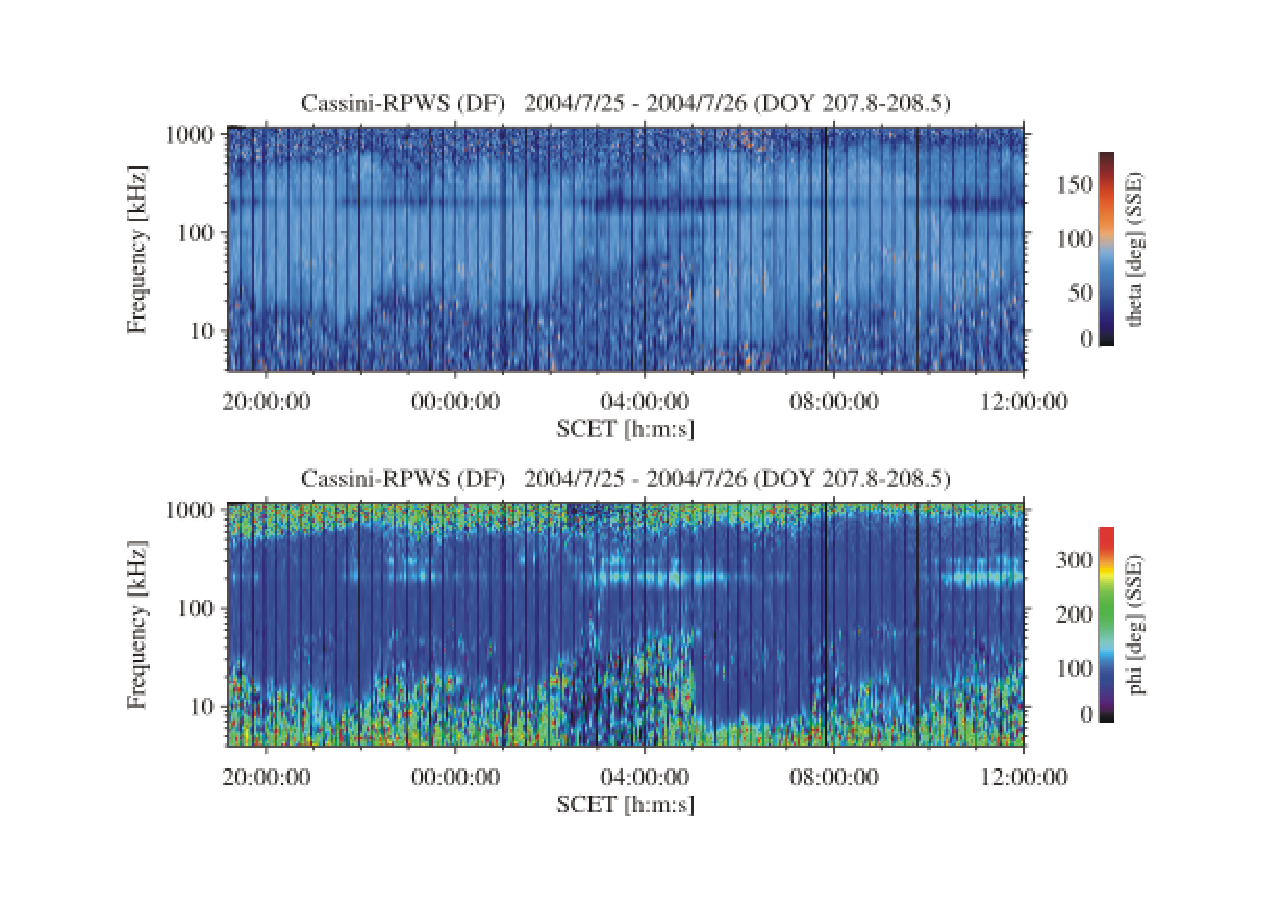
\includegraphics[width=12cm]{uli3.eps}\\
  \caption{The direction of the incident wave, extracted from Cassini data \cite{uli1}}\label{fig_uli1}
\end{figure}

\begin{figure}
  % Requires \usepackage{graphicx}
  \includegraphics[width=12cm]{uli2.eps}\\
  \caption{Stokes parameters extracted from Cassini data \cite{uli1}}\label{fig_uli2}
\end{figure}


\section{\textbf{A numerical method}}

\subsection{Defining the problem}
\paragraph{}
The problem is to solve a nonlinear, overdetermined system of equations. When writing down equations (\ref{auto_corr_allgemein}) to (\ref{im_corr_allgemein}) for all available observables of the SWAVES receiver in the direction finding mode, one ends up with 9 equations. The modeled values are denoted by  $\left\langle V_X V_X^{*} \right\rangle$,  $\left\langle V_Y V_Y^{*} \right\rangle$,  $\left\langle V_Z V_Z^{*} \right\rangle$,  $Re\left\langle V_X V_Y^{*} \right\rangle$, $Re\left\langle V_X V_Z^{*} \right\rangle$, $Re\left\langle V_Y V_Z^{*} \right\rangle$, $Im\left\langle V_X V_Y^{*} \right\rangle$, $Im\left\langle V_X V_Z^{*} \right\rangle$ and $Im\left\langle V_Y V_Z^{*} \right\rangle$ and the measured values by $\widehat{\left\langle V_X V_X^{*} \right\rangle}$,  $\widehat{\left\langle V_Y V_Y^{*} \right\rangle}$,  $\widehat{\left\langle V_Z V_Z^{*} \right\rangle}$,  $\widehat{Re\left\langle V_X V_Y^{*} \right\rangle}$, $\widehat{Re\left\langle V_X V_Z^{*} \right\rangle}$, $\widehat{Re\left\langle V_Y V_Z^{*} \right\rangle}$, $\widehat{Im\left\langle V_X V_Y^{*} \right\rangle}$, $\widehat{Im\left\langle V_X V_Z^{*} \right\rangle}$ and $\widehat{Im\left\langle V_Y V_Z^{*} \right\rangle}$.

\paragraph*{}
Now one can define a function which outputs the sum of the squares of the differences between measured and modeled observables.

\begin{eqnarray}
F(\theta , \phi, \hat{S},\hat{Q},\hat{U},\hat{V})&=&(\left\langle V_X V_X^{*} \right\rangle - \widehat{\left\langle V_X V_X^{*} \right\rangle})^2+\\
&&+(\left\langle V_Y V_Y^{*} \right\rangle - \widehat{\left\langle V_Y V_Y^{*} \right\rangle})^2 +\nonumber \\
&&+(\left\langle V_Z V_Z^{*} \right\rangle - \widehat{\left\langle V_Z V_Z^{*} \right\rangle})^2 +\nonumber \\
&&+(Re\left\langle V_X V_Y^{*} \right\rangle - \widehat{Re\left\langle V_X V_Y^{*} \right\rangle})^2 +\nonumber \\
&&+(Re\left\langle V_X V_Z^{*} \right\rangle - \widehat{Re\left\langle V_X V_Z^{*} \right\rangle})^2 +\nonumber \\
&&+(Re\left\langle V_Y V_Z^{*} \right\rangle - \widehat{Re\left\langle V_Y V_Z^{*} \right\rangle})^2 +\nonumber \\
&&+(Im\left\langle V_X V_Y^{*} \right\rangle - \widehat{Im\left\langle V_X V_Y^{*} \right\rangle})^2 +\nonumber \\
&&+(Im\left\langle V_X V_Z^{*} \right\rangle - \widehat{Im\left\langle V_X V_Z^{*} \right\rangle})^2 +\nonumber\\
&&+(Im\left\langle V_Y V_Z^{*} \right\rangle - \widehat{Im\left\langle V_Y V_Z^{*} \right\rangle})^2 \nonumber
\end{eqnarray}

\paragraph*{}
When written in full length:

\begin{eqnarray}
F(\theta , \phi, \hat{S},\hat{Q},\hat{U},\hat{V})&=&(\hat{S}\eta_0 h_{eff,X}^2[(\hat{Q}+1) A^2_X + \\
&&+(1-\hat{Q}) B^2_X+ 2 \hat{U}A_X B_X]  - \widehat{\left\langle V_X V_X^{*} \right\rangle})^2+\nonumber \\
&&+(\hat{S}\eta_0 h_{eff,Y}^2[(\hat{Q}+1) A^2_Y + \nonumber \\
&&+(1-\hat{Q}) B^2_Y + 2 \hat{U}A_Y B_Y]  - \widehat{\left\langle V_Y V_Y^{*} \right\rangle})^2 +\nonumber \\
&&+(\hat{S}\eta_0 h_{eff,Z}^2[(\hat{Q}+1) A^2_Z +\nonumber \\
&&+ (1-\hat{Q}) B^2_Z+ 2 \hat{U}A_Z B_Z]  - \widehat{\left\langle V_Z V_Z^{*} \right\rangle})^2 +\nonumber \\
&&+(\hat{S}\eta_0 h_{eff,X} h_{eff,Y}[(\hat{Q}+1) A_X A_Y + (1-\hat{Q}) B_X B_Y  +\nonumber \\
&&+  \hat{U} (A_X B_Y + A_Y B_X)] - \widehat{Re\left\langle V_X V_Y^{*} \right\rangle})^2 +\nonumber \\
&&+(\hat{S}\eta_0 h_{eff,X} h_{eff,Z}[(\hat{Q}+1) A_X A_Z + (1-\hat{Q}) B_X B_Z  +\nonumber \\
&&+  \hat{U} (A_X B_Z + A_Z B_X)] - \widehat{Re\left\langle V_X V_Z^{*} \right\rangle})^2 +\nonumber \\
&&+(\hat{S}\eta_0 h_{eff,X} h_{eff,Z}[(\hat{Q}+1) A_Y A_Z + (1-\hat{Q}) B_Y B_Z  +\nonumber \\
&&+  \hat{U} (A_Y B_Z + A_Z B_Y)] - \widehat{Re\left\langle V_Y V_Z^{*} \right\rangle})^2 +\nonumber \\
&&+(-\hat{S}\eta_0 h_{eff,X} h_{eff,Y} \hat{V}[-A_X B_Y + A_Y B_X ] - \widehat{Im\left\langle V_X V_Y^{*} \right\rangle})^2 +\nonumber \\
&+&(-\hat{S}\eta_0 h_{eff,X} h_{eff,Z} \hat{V}[-A_X B_Z + A_Z B_X ] - \widehat{Im\left\langle V_X V_Z^{*} \right\rangle})^2+ \nonumber\\
&+&(-\hat{S}\eta_0 h_{eff,Y} h_{eff,Z} \hat{V}[-A_Y B_Z + A_Z B_Y ] - \widehat{Im\left\langle V_X V_Z^{*} \right\rangle})^2 \nonumber
\end{eqnarray}


\paragraph*{}
This function must be greater or equal zero. It \emph{is} zero when the parameters have exactly the values of the solution of the problem. Hence, by finding the minimum of this function, one can get as close to the solution as possible. From a geometric viewpoint the function is a six dimensional hyper surface. There are methods for minimization problems on hyper surfaces, one of which is recommended for the DF problem.

\subsection{Finding the minimum of a function of multiple parameters}
\paragraph*{}
A Taylor polynom of order 2, approximating a multidimensional function at $\textbf{x}_0$ has the equation

\begin{equation}
F(\textbf{x} )\simeq F( \textbf{x}_0) + \delta \textbf{ x}^T \nabla F( \textbf{x}_0 )  + \frac{1}{2}  \delta \textbf{ x}^T \textbf{G}( \textbf{x}_0 ) \delta \textbf{x}
\end{equation}

\paragraph*{}
$\textbf{G}( \textbf{x} )$ is the Hessian Matrix with elements

\begin{equation}
G_{ij}(\textbf{x} )=\frac{\partial^2 F}{\partial x_i \partial x_j}(\textbf{x})
\end{equation}

\paragraph*{}
At a minimum, the following must be true:

\begin{itemize}
\item  $\nabla F( \textbf{x} )=0$
\item  $\textbf{G}( \textbf{x} )$ is positive definite
\end{itemize}

\paragraph*{}
The first criterion ensures that it is a stationary point, the second that it is a minimum. The normal method for testing \textbf{G} for positive definiteness is to compute its eigenvalues. But this procedure is not practicable for large matrices. There is an other method, the Cholesky Method, which is better suited for this task.

\paragraph*{}
\shadowbox{\parbox{12cm}{Cholesky Theorem\\
\\
A symmetric matrix \textbf{A} is called positive definite, if, and only if, it has a Cholesky Decomposition $\textbf{A}=\textbf{LL}^T$, such that \textbf{L} is a low triangular matrix, all elements of \textbf{L} are real and all elements of the main diagonal are different from zero.}}

\paragraph*{}
\textbf{L} is the low triangular matrix. Its elements are:

\begin{eqnarray}
l_{ii}&=&\left( a_{ii}-\sum^{i-1}_{k=1} l^2_{ik} \right) ^\frac{1}{2}\bigskip (i=1,...,n)\\
l_{ji}&=&\frac{1}{l_{ii}}\left( a_{ij}-\sum^{i-1}_{k=1} l_{ik} l_{jk}\right) \bigskip (i=1,...,n;j=i+1,...,n)
\end{eqnarray}

\paragraph*{}
The convention has to be taken into account that the sum of non-existent terms is zero. One has to compute the elements in correct order. What makes the Colesky Decomposition so practicable is the fact that it is possible to solve an equation of the form $\textbf{Ax}=\textbf{b}$ while performing the decomposition. Besides, it is faster and more stable than the LU\footnote{The LU decomposition is a standard method of numerical analysis that expresses a matrix as the product of a lower and an upper triangular matrix. These matrices can be used to solve a linear system of equations. The method is, in general, falster than other methods.} decomposition, for instance.
%
\subsection{The Newton-Raphson Method}
\paragraph*{}
One of the methods, useful for minimization, is the Newton-Raphson Method (NRM). It has the advantage that it uses not only the gradient, but also information about the curvature, that is the Hessian matrix, for finding the minimum in an efficient way. To be able to use the NRM, the function to be minimized, has to be smooth, well behaved and differentiable to the second order.

\subsubsection{The one-dimensional case}
\paragraph*{}
Finding a minimum of a one-dimensional function is done by looking for the point where $f'=0$. The NRM is based upon the Taylor approximation of first order at around point $x_r$.

\begin{equation}
h(x)\simeq h(x_r)+(x-x_r)h'(x_0)
\end{equation}

\paragraph*{}
At the zero $h(x)=0$, hence we seek $x_{r+1}$ such that

\begin{equation}
0=h(x_r)+(x_{r+1}-x_r)h'(x_r)
\end{equation}

\paragraph*{}
Solving for $x_{r+1}$:

\begin{equation}
x_{r+1}=x_r-\frac{h(x_r)}{h'(x_r)}=x_r-\frac{f'(x_r)}{f''(x_r)}
\end{equation}

\paragraph*{}
This is the Newton Raphson Formula for the computation of $f'(x)=0$.

\subsubsection*t{The multidimensional NRM}
\paragraph*{}
In case of an n-dimensional problem, one can determine a stationary point by solving the following equation.

\begin{equation}
\nabla f(\textbf{x})=0
\end{equation}

\paragraph*{}
Or, when written as components:

\begin{equation}
\frac{\partial f}{\partial x_i}(\textbf{x})=0 \qquad(i=1,...,n)
\end{equation}

\paragraph*{}
So a system of n equations is to be solved. The Newton-Raphson Formula for a system like $\textbf{h}(\textbf{x})=\textbf{0}$ is

\begin{equation}
\textbf{x}_{r+1}=\textbf{x}_r-\textbf{J}(\textbf{x}_r)^{-1}\textbf{h} (\textbf{x}_r) \label{nrm_multidim}
\end{equation}

\paragraph*{}
\textbf{J} is the Jacobi matrix for \textbf{h}. The Jacobi matrix for $\nabla f$ is the Hessian matrix $G$, so (\ref{nrm_multidim}) becomes

\begin{equation}
\textbf{x}_{r+1}=\textbf{x}_r-\textbf{G}(\textbf{x}_r)^{-1}\nabla f(\textbf{x}_r)
\end{equation}

\paragraph*{}
which can be transformed to give

\begin{equation}
\textbf{G}(\textbf{x}_r)\Delta_r=-\nabla f (\textbf{x}_r ) \label{nrm_multidim_dispacement}
\end{equation}

\paragraph*{}
This equation can be used to compute the \emph{displacement vector} $\Delta_r $ and with use of the relation

\begin{equation}
\textbf{x}_{r+1}=\textbf{x}_r + \Delta_r
\end{equation}

\paragraph*{}
the iterative scheme is complete. Equation (\ref{nrm_multidim_dispacement}) can be solved best by using the Cholesky Decomposition. One has to solve

\begin{equation}
\textbf{Lc}=-\nabla f
\end{equation}

\paragraph*{}
and

\begin{equation}
\textbf{L}^T \textbf{x}=\textbf{c}
\end{equation}

\paragraph*{}
There are, however, some drawbacks when using the NRM:

\begin{itemize}
\item The method does not always converge, when the starting point is not selected near enough to the minimum, or one ends up at a local minimum.
\item One has to compute $\nabla f$ and $\textbf{G}$ at each iteration.
\item The system has to be fully solved at each iteration.
\item The method fails if \textbf{G} is not positive definite.
\end{itemize}

\paragraph*{}
There are a lot of other, more advanced methods with better performance which can be found in specialized papers or textbooks. The NRM is one of the simplest and clearest which has a reasonably good performance and stability. That is the reason, why I chose it representatively. Unfortunately, it is not possible to ensure that it converges to the global minimum instead a local minimum, without use of further methods, like a grid method to find the starting point. If one uses an n by n by n...and so on grid, one ends up with $n^6$ nodes at which the function has to be evaluated. This can be time consuming and one can think of function topologies where even this brute force method does not work. I doubt that DF can be automatized by use of the method described in this section. Details of the methods described here and other possible methods can be found in \cite{burdenfaires} and \cite{recipes}.

\chapter{\textbf{Determination of the effective length vectors of the SWAVES antennas}}
\section{\textbf{Introduction}}
\paragraph*{}
Together with the Radio Science team of the Space Research Institute Graz led by Prof. H.O. Rucker, I performed numerical calculations, using ASAP and the ASAP toolbox, to determine the characteristics of the three antennas of the STEREO/SWAVES experiment. The results of the second refinement of modeling the spacecraft, which is internally called \emph{Design 2}, is presented in this thesis. It was the first model, which was constructed from the spacecraft plans and is therefore the first model to be expected to provide a realistic outcome. \cite{vogl_01}, \cite{vogl_04}, \cite{cassini2}, \cite{cassini3}, \cite{cassini} \cite{marsis} and \\
\cite{marsis2} can be referenced to find similar works on other spacecraft, as well as a summery \cite{ruckerundi05}.

\section{\textbf{The spacecraft}}
\subsection{Characteristics}

\paragraph*{}
A characteristic of the spacecraft is a certain degree of
asymmetry. In contrast to many other spacecraft, the solar panels
are positioned at different longitudinal distances at the
spacecraft hull. Additionally the spacecraft consist of an about
6 meters long boom, and a turnable high gain antenna, which are also two
prominent features we expected an influence of the antenna
characteristics. The boom is divided into 4 sections with
different diameters and has great influence upon
the effective length vectors of the antennas.

\paragraph*{}
The used, spacecraft fixed, reference frame is defined in a way to be spacecraft fixed with the positive x-axis in a direction which will point to the sun during most of the time, so the antennas are mounted on the side of the hull which points to the negative x-axis. The solar panels point to the positive and negative y- axis and the z-axis is defined to complete the right handed cartesian frame.

\paragraph*{}
For the description of the direction of the antennas we chose to employ a spherical polar system which has the positive X-axis as polar axis. The angle $\zeta$ is the angle between the positive X-axis and the antenna, and $\xi$ is the azimuthal angle around the X-axis, where E1 is defined to have $\xi=0$.

\paragraph*{}
The direction of the
boom defines the negative x-axis. There are 3 orthogonal monopole antennas,
which are called E1, E2 and E3, each 6 meters
long. They are directed about $125.26^\circ$ from the x-axis. The
difference in azimuth is $120^\circ$. The azimuth of antenna
E1 defines the azimuth of $0^\circ$. It is expected, that the boom has an
effect to push the 3 electrical antennas away from the boom's position. This effect is
increased by the high gain antenna, which is located near the
boom. The panels are expected to push the effective length vectors
towards the negative x-axis.

\paragraph*{}
The antennas will be directed away from the sun, so that they
remain out of view of the sunward looking instruments on the
spacecraft. Thus, the most interesting direction of incident waves
is the positive x-axis, which is another reason for which we
believe that the spacecraft will have a massive influence upon the
characteristics of the antennas above the quasi-static regime. The
antennas will be used in a frequency range between 30kHz and
16MHz.

\paragraph*{}
The two spacecraft, A and B are almost identical, apart of some small differences of their instrumentation. The only difference that can be modeled within the limitations of ASAP is the second ring, which is mounted on the hull of spacecraft B on the positive x side, and is not existent on spacecraft A.

\begin{table}[h]
\centering
\label{tab_base_caps55}
\caption{Base capacitances}
\begin{tabular}{|c|c|c|c|}
 \hline
% after \\: \hline or \cline{col1-col2} \cline{col3-col4} ...
\textbf{Antenna} & \textbf{E1} & \textbf{E3} & \textbf{E3} \\
\hline
\textbf{Antennas/pF} & 55 & 55 & 55 \\
\textbf{Receivers/pF}& 25 & 25 & 25 \\
\textbf{Cables/pF} & 10 & 10 & 10 \\
\hline
\textbf{Entire Capacitance/pF} & 90 & 90 & 90 \\
\hline\end{tabular}
\end{table}

\paragraph*{}
With information about the base capacitances of antennas, coax cables and receivers, we were able to calculate and include the base impedances at the second run of the computations. The actual values are tabulated in Table 5.1. \\


\begin{figure}[h]
  % Requires \usepackage{graphicx}
  \includegraphics[width=12cm]{stereo1.eps}\\
  \caption{The STEREO spacecraft}\label{fig_stereo}
\end{figure}

\subsection{The model}
The first three models of the Stereo spacecraft consist of the following parts:\\
\\
\begin{itemize}
\item Hull
\item Asymmetric solar panels
\item High Gain Antenna
\item SWAVES Antennas
\item Boom
\item 2 Rings mounted on the hull
\end{itemize}

\paragraph*{}
The parts were made of fundamental structure items, the basic building blocks of the Matlab-ASAP toolbox. Size and position of the parts were measured from the relevant construction plans. The proximal part of
the tapered boom is modeled as prism with triangular base. Figures \ref{fig_D2_A_Oblique} to \ref{fig_D2_A_Z_View} show the model in three side views and from an oblique angle. The description \emph{N-View}, where N can be + or -, X, Y or Z, means that the point of view is located in direction of the N-axis in relation to the model.\\


\begin{figure}
  % Requires \usepackage{graphicx}
  \begin{center}
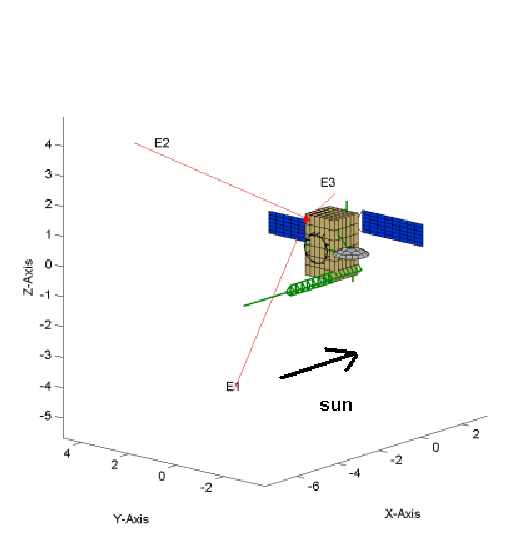
\includegraphics[width=8cm]{SpaceCraftD2HGA0Oblique.eps}\\
  \caption{Spacecraft A}\label{fig_D2_A_Oblique}
  \includegraphics[width=8cm]{SpaceCraftD2HGA0-XView.eps}\\
  \caption{Spacecraft A: X-View}\label{fig_D2_A_X_View}\end{center}
\end{figure}

\begin{figure}
  % Requires \usepackage{graphicx}
  \begin{center}
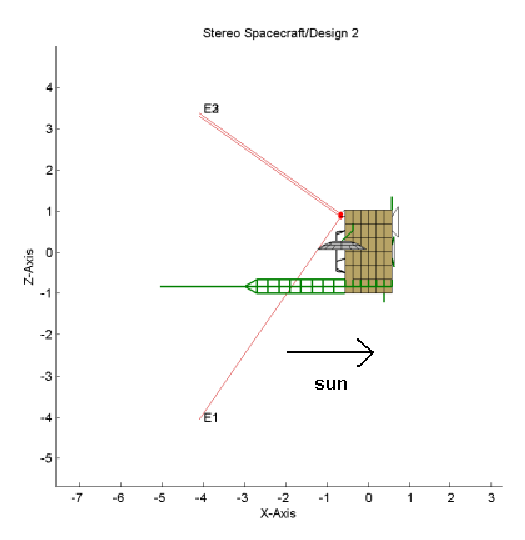
\includegraphics[width=8cm]{SpaceCraftD2HGA0-YView.eps}\\
  \caption{Spacecraft A: Y-View}\label{fig_D2_A_Y_View}
  \includegraphics[width=8cm]{SpaceCraftD2HGA0ZView.eps}\\
  \caption{Spacecraft A: Z-View}\label{fig_D2_A_Z_View}\end{center}
\end{figure}

\section{\textbf{The Computation}}

\subsection{Computation of the effective length vectors}

\paragraph*{}
As first step, we computed the currents at frequencies from 100kHz
to 16MHz, with a spacing of 100kHz, each frequency with 19 different angles of the HGA dish. The range of the HGA dish can be seen on figure \ref{fig_hgarange} as if there would be multiple exposures of a photograph. This computation was performed by the ASAP program. Using these data, the impedances, admittances and effective length vectors can easily be computed with the
toolbox devised at the Space research Institute and updated to be suitable for the specific task of analyzing the antennas of SWAVES.

\begin{figure}
\begin{center}
  % Requires \usepackage{graphicx}
  \includegraphics[width=8cm]{showallhgaangles.eps}\\
  \caption{Range of HGA angle}\label{fig_hgarange}
\end{center}
\end{figure}

\section{\textbf{Calculations}}
\paragraph*{}
Figures \ref{fig_Heff_D2_A_X_ViewCap}-\ref{fig_Heff_D2_B_Z_ViewCap} show plots of the effective length vectors of spacecraft A and B in turn. The frequency used for these plots is 500kHz, being well in the quasistatic regime. The direction of the incident wave is from the positive x-axis, simulating radiation from the sun.\\

\begin{figure}
  \begin{center}
    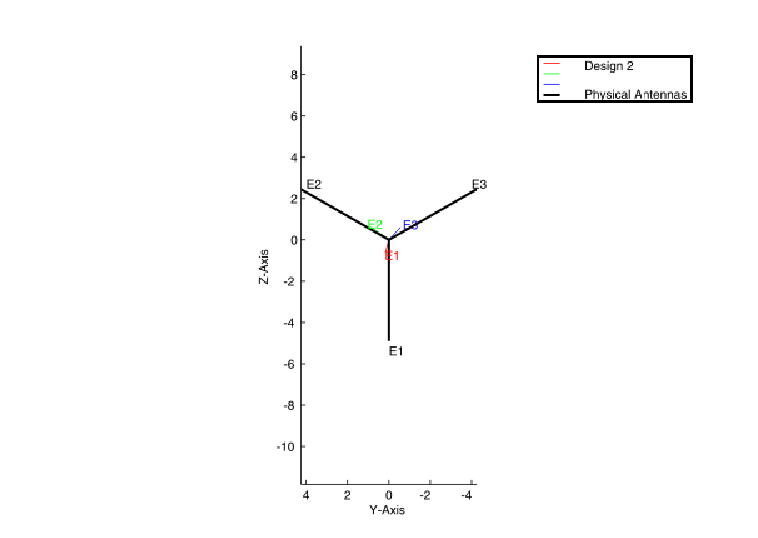
\includegraphics[width=12cm]{HeffD2HGA0-500kHz-XViewCap.eps}\\
    \caption{Spacecraft A: Effective Length Vectors,X-View/ Capacitances included}\label{fig_Heff_D2_A_X_ViewCap}
  \end{center}
\end{figure}


\begin{figure}
 \begin{center}
 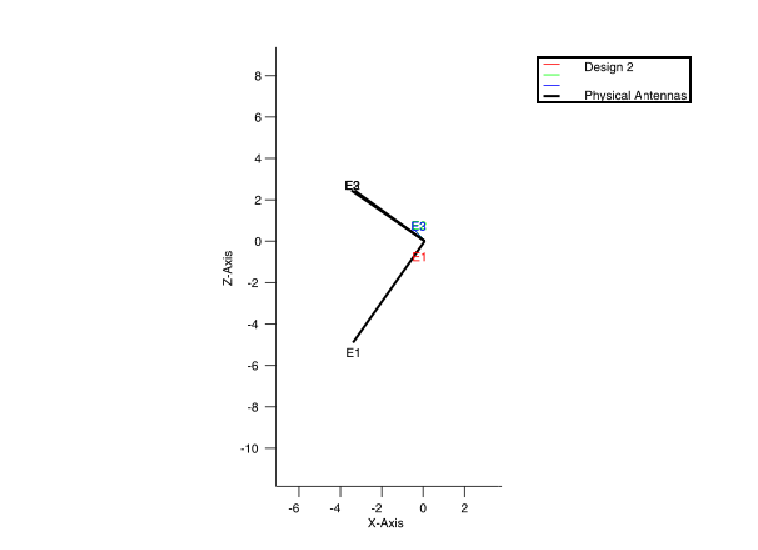
\includegraphics[width=12cm]{HeffD2HGA0-500kHz-YViewCap.eps}\\
    \caption{Spacecraft A: Effective Length Vectors,Y-View/ Capacitances included}\label{fig_Heff_D2_A_Y_ViewCap}\end{center}
\end{figure}

\begin{figure}
        \begin{center}
        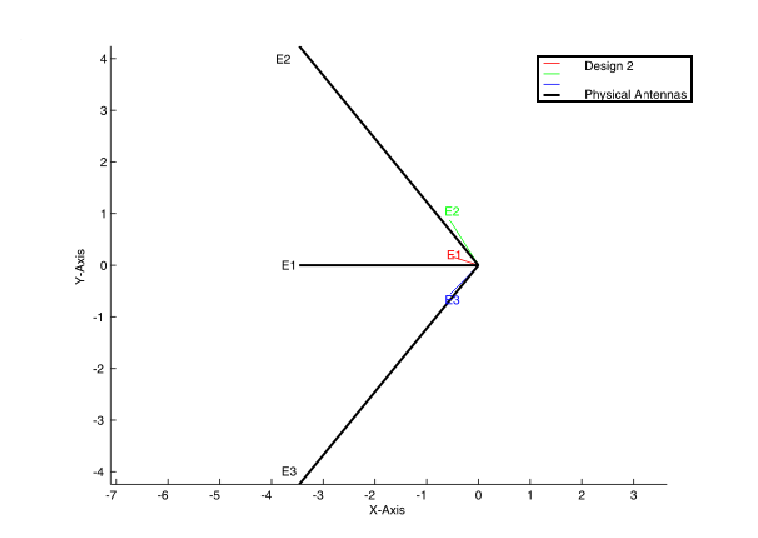
\includegraphics[width=12cm]{HeffD2HGA0-500kHz-ZViewCap.eps}\\
        \caption{Spacecraft A: Effective Length Vectors,Z-View/ Capacitances included}\label{fig_Heff_D2_A_Z_ViewCap}
    \end{center}
\end{figure}

\begin{figure}
  \begin{center}
    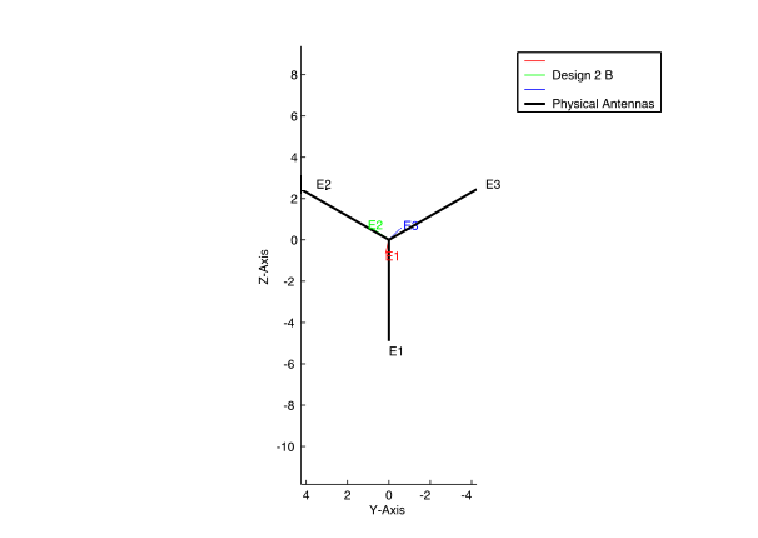
\includegraphics[width=12cm]{HeffD2HGA0-500kHz-XViewCap_B.eps}\\
    \caption{Spacecraft B: Effective Length Vectors,X-View/ Capacitances included}\label{fig_Heff_D2_B_X_ViewCap}
  \end{center}
\end{figure}


\begin{figure}
 \begin{center}
 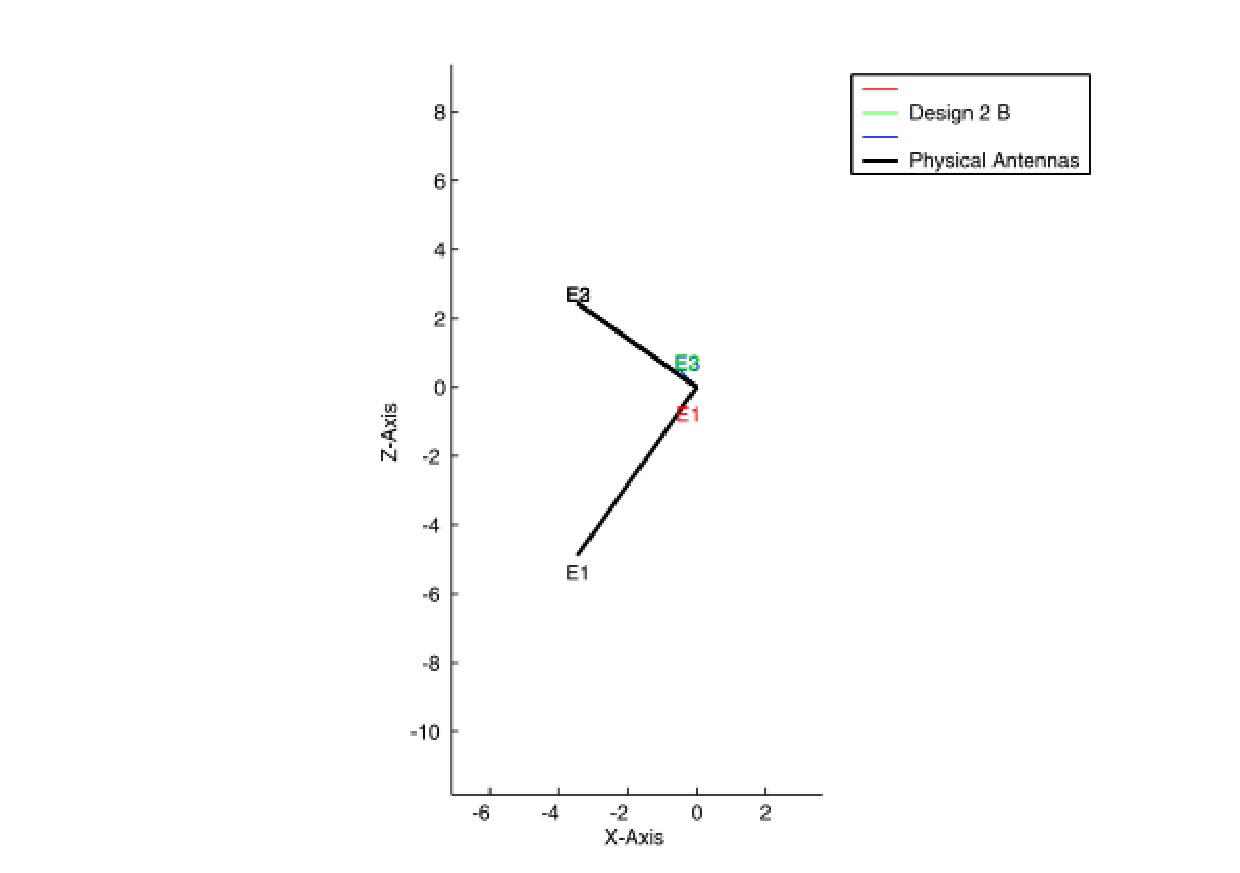
\includegraphics[width=12cm]{HeffD2HGA0-500kHz-YViewCap_B.eps}\\
    \caption{Spacecraft B: Effective Length Vectors,Y-View/ Capacitances included}\label{fig_Heff_D2_B_Y_ViewCap}\end{center}
\end{figure}

\begin{figure}
        \begin{center}
        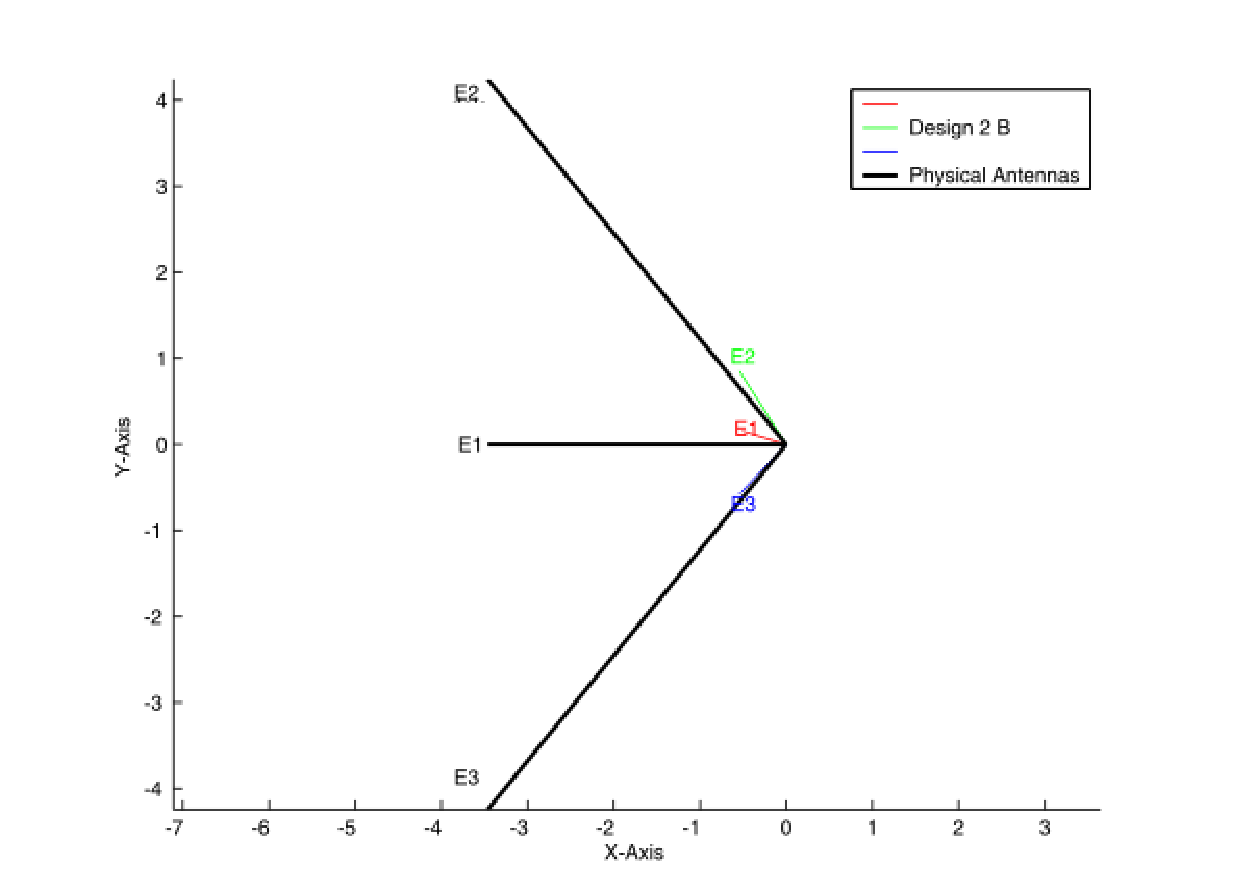
\includegraphics[width=12cm]{HeffD2HGA0-500kHz-ZViewCap_B.eps}\\
        \caption{Spacecraft B: Effective Length Vectors,Z-View/ Capacitances included}\label{fig_Heff_D2_B_Z_ViewCap}
    \end{center}
\end{figure}
\paragraph*{}
Table 5.2 shows the information in tabulated form. For comparison, the lengths and orientation information of the physical antennas are also added.

% table
\begin{table}[h]
\centering
\label{tab_heff}
\caption{Effective length vectors at 500kHz}
\begin{tabular}{|c|c|c|c|c|}
\hline
 &  & Spacecraft A & Spacecraft B & Physical antennas \\
\hline E1 &
 \begin{tabular}{c}
\hline Length/m \\
\hline $\zeta/^\circ$ \\
\hline $\xi/^\circ$ \\
\hline
\end{tabular}
&
\begin{tabular}{c}
\hline  0.83\\
\hline  128.3\\
\hline  15.0\\
\hline
\end{tabular}
&
\begin{tabular}{c}
\hline  0.84\\
\hline  127.2\\
\hline  13.3\\
\hline
\end{tabular}
&
\begin{tabular}{c}
\hline 6.00 \\
\hline 125.26 \\
\hline 0.0 \\
\hline
\end{tabular}  \\
\hline E2 &
\begin{tabular}{c}
\hline Length/m \\
\hline $\zeta/^\circ$ \\
\hline $\xi/^\circ$ \\
\hline
\end{tabular}
&
\begin{tabular}{c}
\hline  1.21\\
\hline  117.1\\
\hline  125.8\\
\hline
\end{tabular}
&
\begin{tabular}{c}
\hline  1.18\\
\hline  117.4\\
\hline  125.2\\
\hline
\end{tabular}
&
\begin{tabular}{c}
\hline 6.00 \\
\hline 125.26 \\
\hline 120.0 \\
\hline
\end{tabular}  \\
\hline E3 &
 \begin{tabular}{c}
\hline Length/m \\
\hline $\zeta/^\circ$ \\
\hline $\xi/^\circ$ \\
\hline
\end{tabular}
&
\begin{tabular}{c}
\hline  0.99\\
\hline  123.5\\
\hline  -137.2\\
\hline
\end{tabular}
&
\begin{tabular}{c}
\hline  0.98\\
\hline  123.3\\
\hline  -135.4\\
\hline
\end{tabular}
&
\begin{tabular}{c}
\hline 6.00m \\
\hline 125.26� \\
\hline -120.0� \\
\hline
\end{tabular}  \\
\hline
\end{tabular}
\end {table}

\paragraph*{}
The quasistatic results were in full concurrence with our expectations. All electric antennas have lengths which are near the half
length of the physical antennas, as expected by theory for
monopole antennas that are small in relation to the wavelength.
The influence of the capacitances on the effective length vectors seems to be quite substantial.
Furthermore, it can clearly be seen that the solar panels push
the electric antennas towards the negative
x-axis with a counteracting influence of the boom. The difference between the two spacecraft, although not large, is definitely existent.

\subsection{Variation of the effective length vectors with frequency and direction}

\paragraph*{}
As mentioned before, direction finding is only possible in the lower frequency regions. At higher frequencies, the effective length vectors become complex and dependent of frequency and direction of incidence. The variability of the real part of the effective length vectors can be easily seen on plots \ref{fig_heff_dist_D2_A_Z_View_caps} and \ref{fig_heff_dist_D2_B_Z_View_caps}. The plot was constructed by choosing 26 different directions and computing the effective length vectors for each frequency and each direction. The real part of all effective length vectors were plotted. The frequency is color coded. The imaginary parts of the vectors were ignored. The 26 sample directions are shown in figures \ref{fig_sample_z} and \ref{fig_sample_oblique} for reference. We did not include diagrams of the X- and Y-view, because they look exactly the same as the Z-view. The reason for the erratic behavior is the resonance at 14 MHz. For comparison, figures \ref{fig_heff_dist_D2_A_Z_View_caps2}, \ref{fig_heff_dist_D2_A_Z_View_caps3}, \ref{fig_heff_dist_D2_B_Z_View_caps2}, and \ref{fig_heff_dist_D2_B_Z_View_caps3} show plots, generated the same way, but with a frequency range up to only 13MHz and 12MHz, respectively. The variability of the effective axis seems to be much more well behaved at those lower frequencies.\\
\\

\begin{figure}
\begin{center}
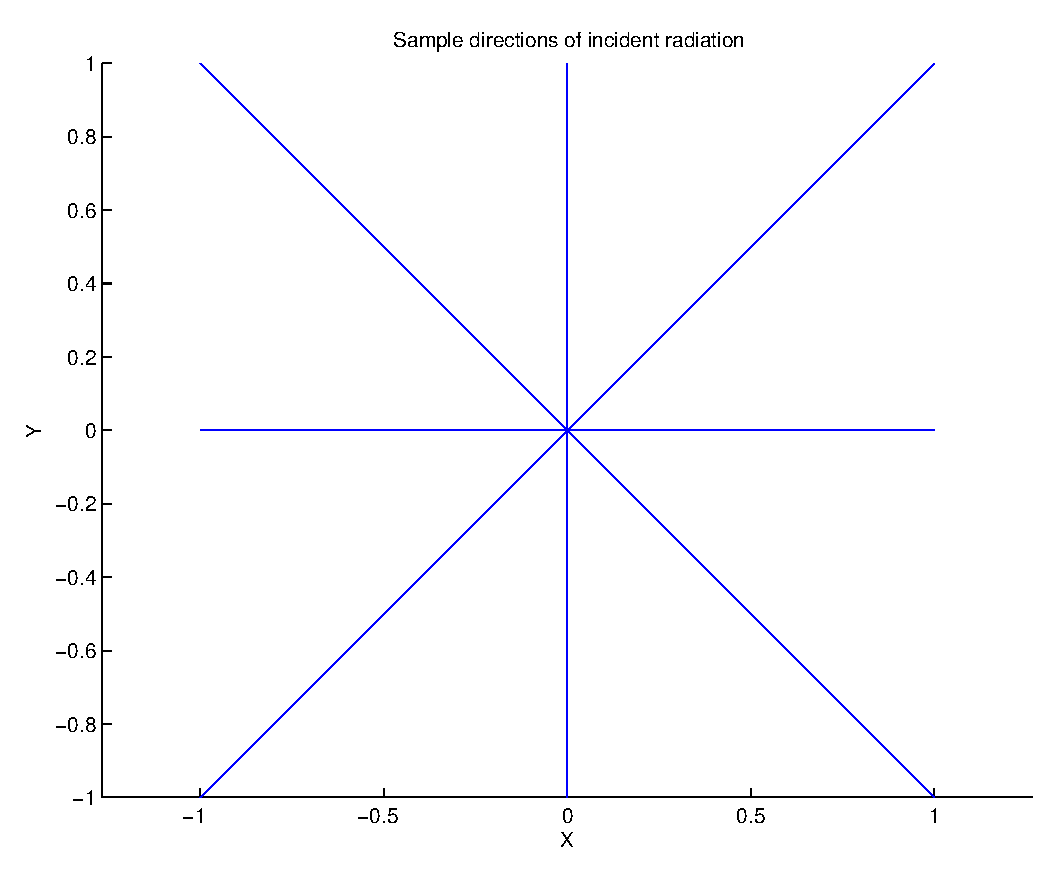
\includegraphics[width=8cm]{SampleDirection_ZView.eps}\\
\caption{Sample directions/Z View}\label{fig_sample_z}
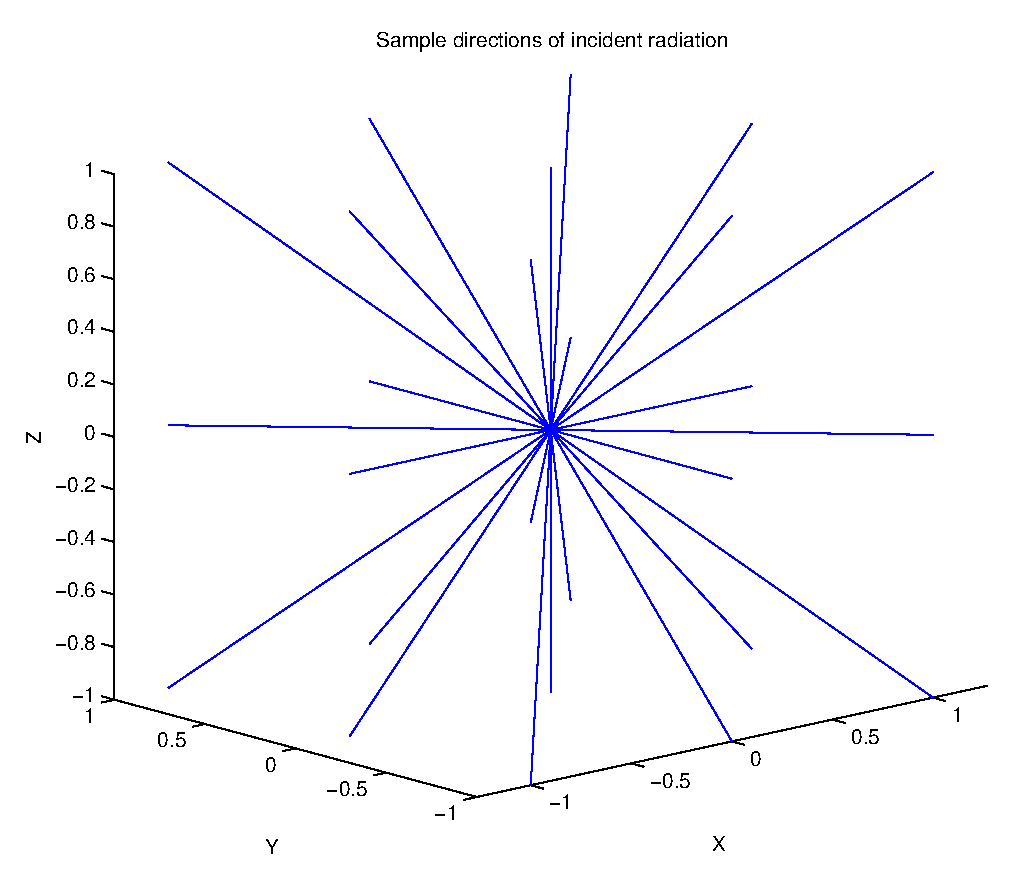
\includegraphics[width=8cm]{SampleDirection_oblique.eps} \\
\caption{Sample directions/Oblique View}\label{fig_sample_oblique}
\end{center}
\end{figure}

\begin{figure}
\begin{center}
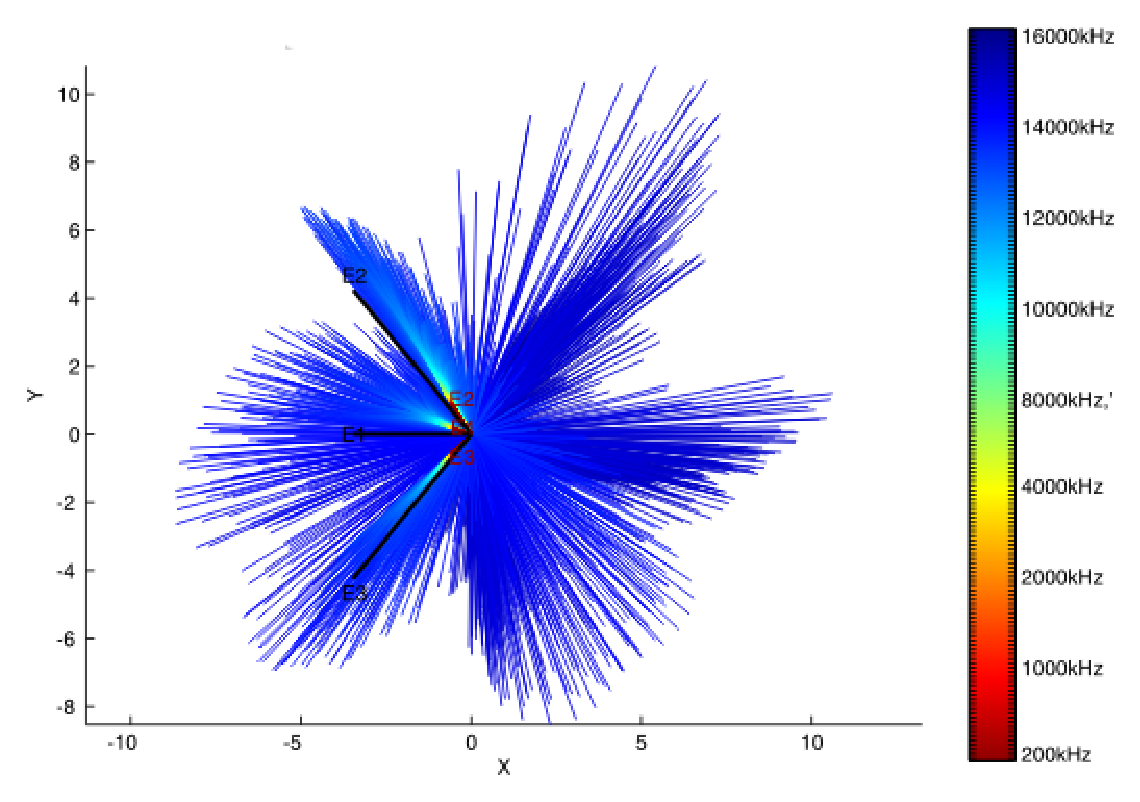
\includegraphics[scale=0.65]{HeffVerteilungD2-ZView_caps.eps} \\
\caption{The spatial distribution of the real parts of the effective length vectors of the design 2 model with capacitances included-frequency up to 16MHz/Z View }\label{fig_heff_dist_D2_A_Z_View_caps}
\end{center}
\end{figure}

\begin{figure}
\begin{center}
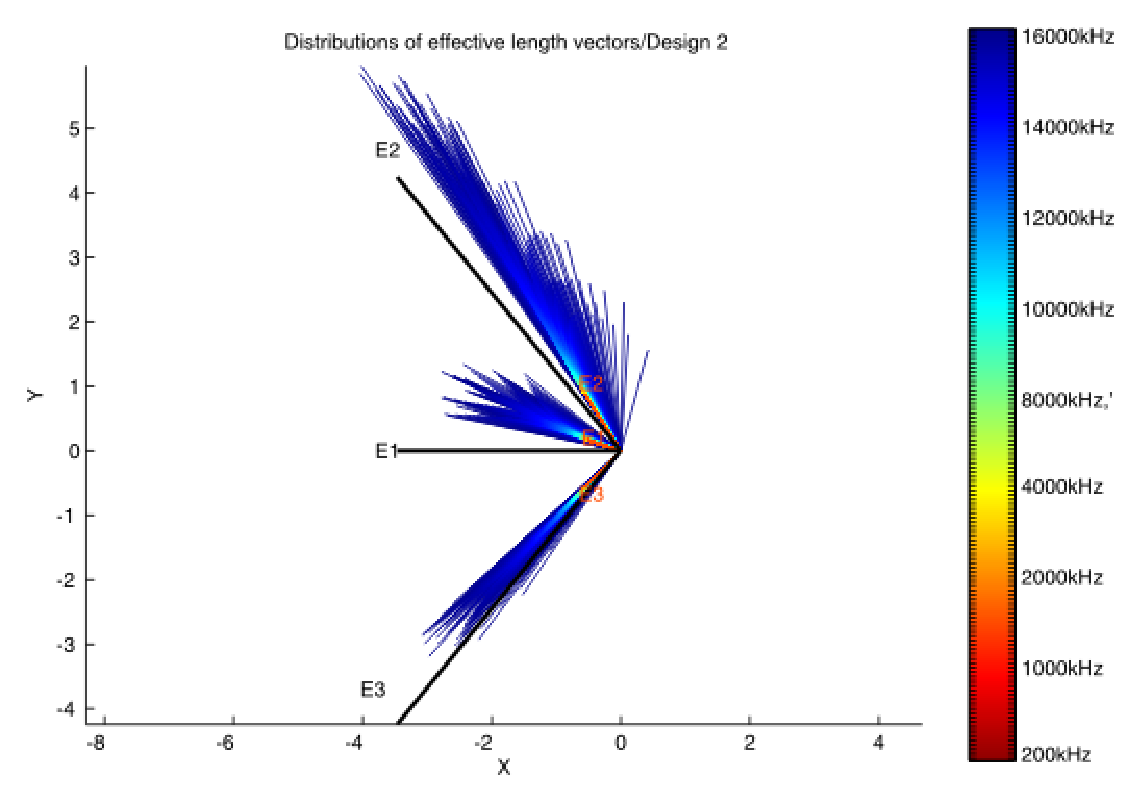
\includegraphics[scale=0.65]{HeffVerteilungD2-ZView_caps2.eps} \\
\caption{The spatial distribution of the real parts of the effective length vectors of the design 2 model with capacitances included-frequency up to 13MHz/Z View }\label{fig_heff_dist_D2_A_Z_View_caps2}
\end{center}
\end{figure}

\begin{figure}
\begin{center}
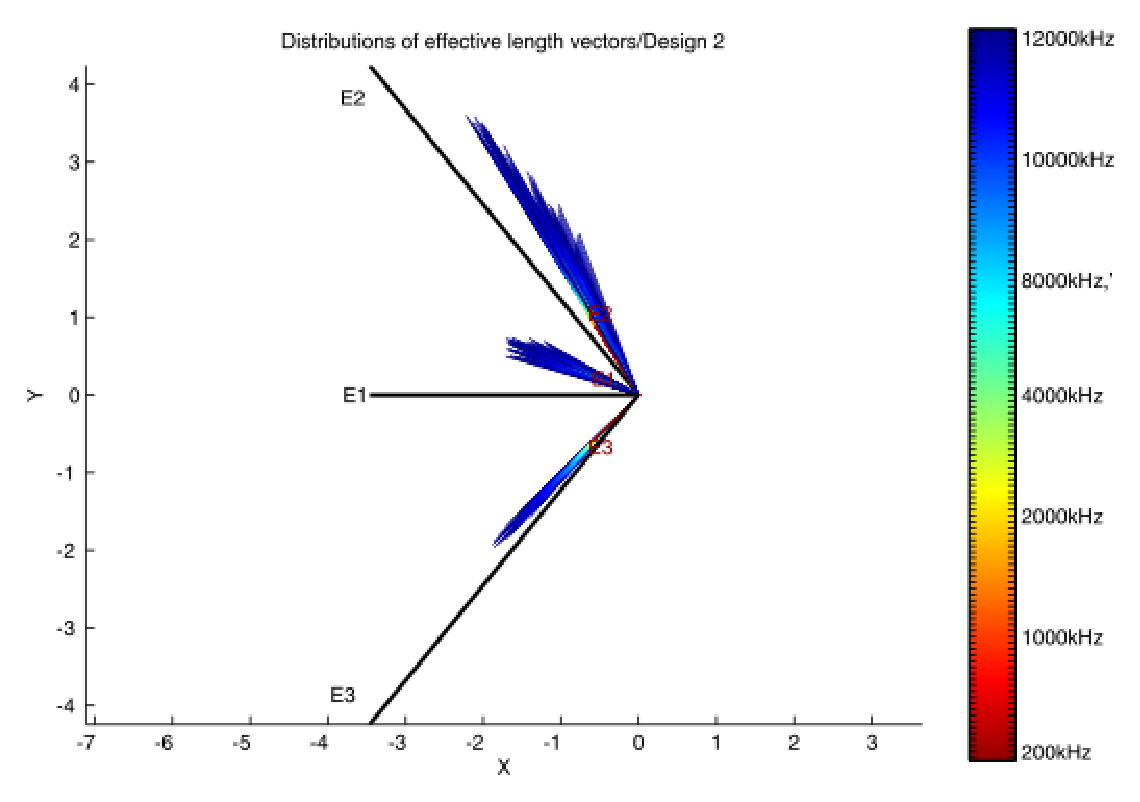
\includegraphics[scale=0.65]{HeffVerteilungD2-ZView_caps3.eps} \\
\caption{The spatial distribution of the real parts of the effective length vectors of the design 2 model with capacitances included-frequency up to 12MHz/Z View }\label{fig_heff_dist_D2_A_Z_View_caps3}
\end{center}
\end{figure}

\begin{figure}
\begin{center}
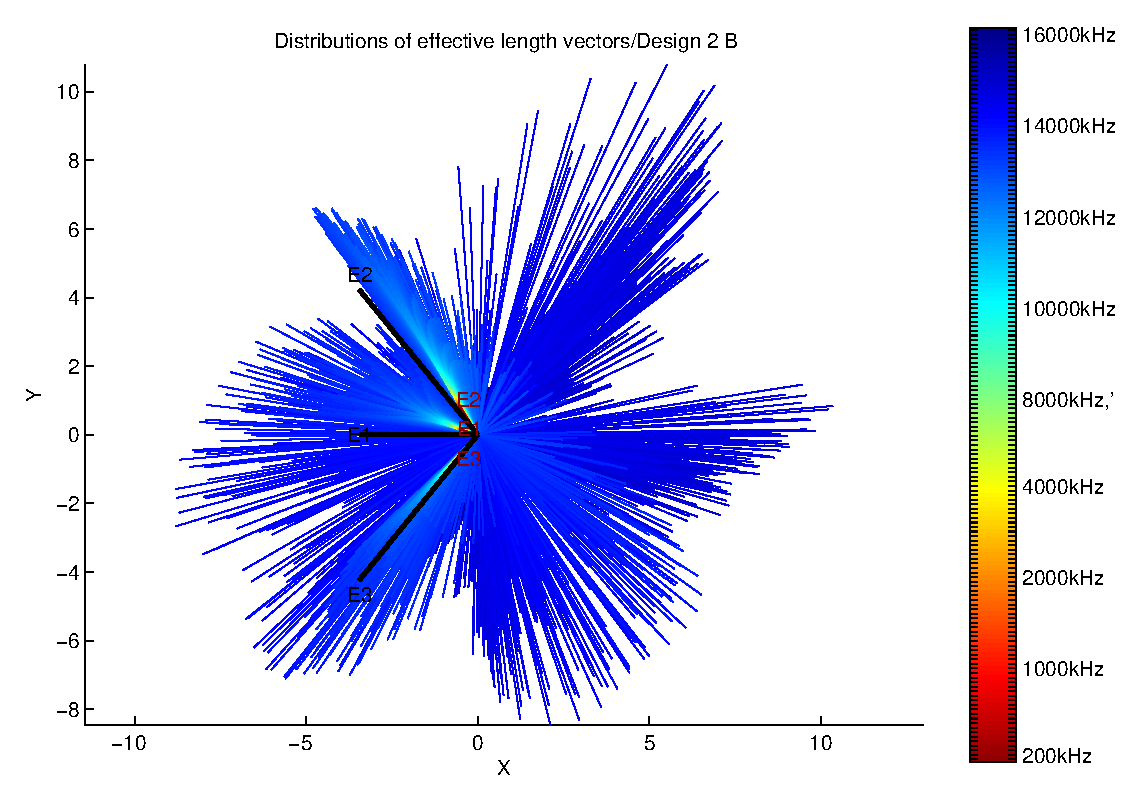
\includegraphics[scale=0.65]{HeffVerteilungD2-ZView_B_caps.eps} \\
\caption{The spatial distribution of the real parts of the effective length vectors of the design 2 model B with capacitances included-frequency up to 16MHz/Z View }\label{fig_heff_dist_D2_B_Z_View_caps}
\end{center}
\end{figure}

\begin{figure}
\begin{center}
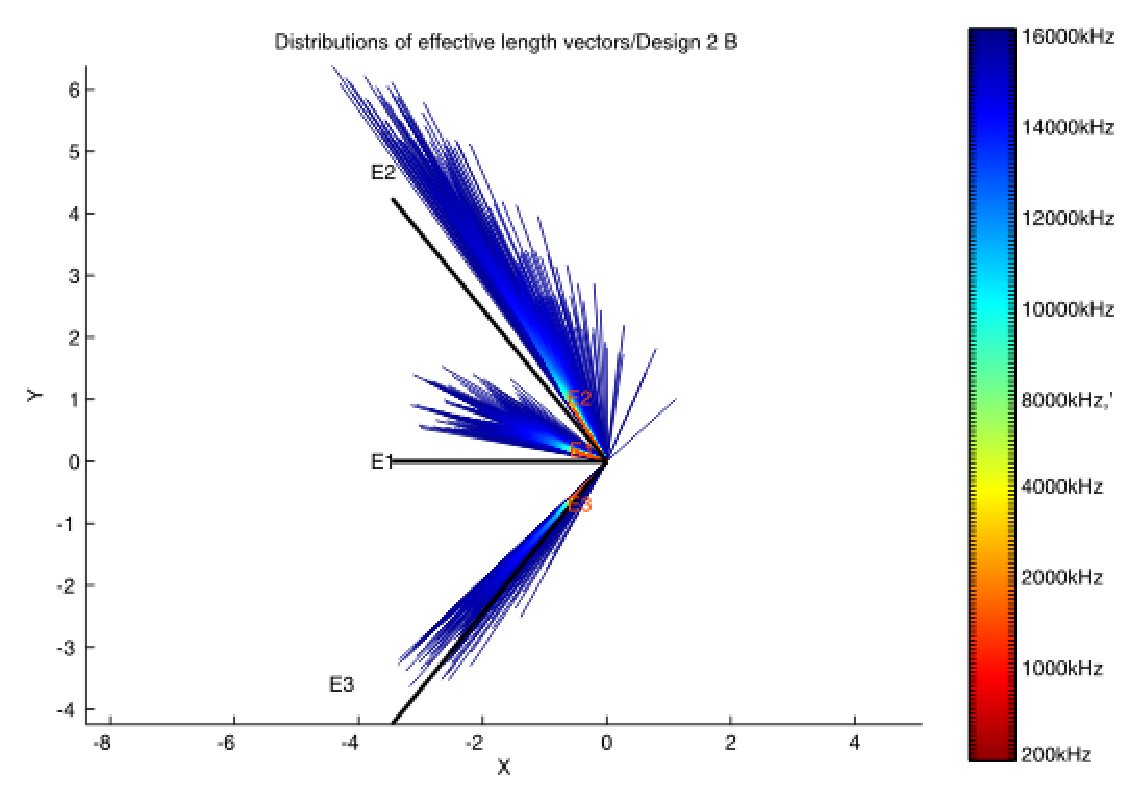
\includegraphics[scale=0.65]{HeffVerteilungD2-ZView_B_caps2.eps} \\
\caption{The spatial distribution of the real parts of the effective length vectors of the design 2 model B with capacitances included-frequency up to 13MHz/Z View }\label{fig_heff_dist_D2_B_Z_View_caps2}
\end{center}
\end{figure}

\begin{figure}
\begin{center}
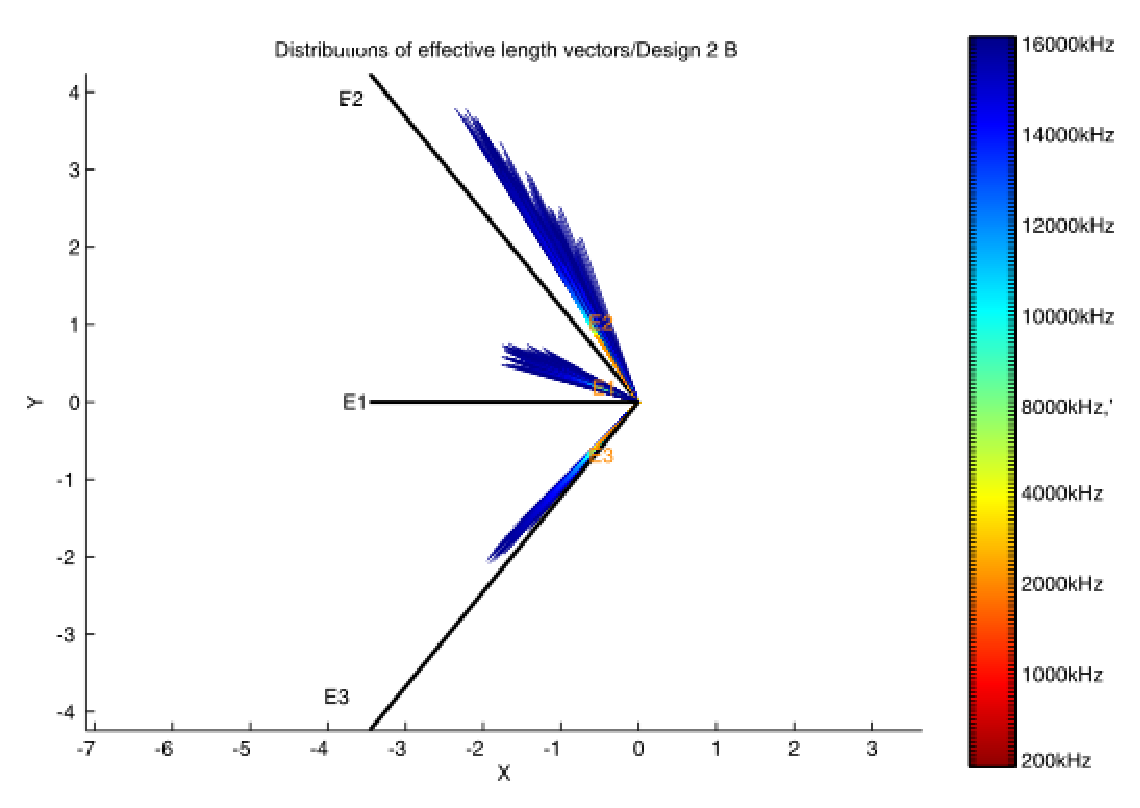
\includegraphics[scale=0.65]{HeffVerteilungD2-ZView_B_caps3.eps} \\
\caption{The spatial distribution of the real parts of the effective length vectors of the design 2 model B with capacitances included-frequency up to 12MHz/Z View }\label{fig_heff_dist_D2_B_Z_View_caps3}
\end{center}
\end{figure}

\paragraph*{}
A method to quantify these plots is to compute the standard
deviation of the parameters. Due to the fact that the components
of the vectors are complex, the normal procedure of computing the
standard deviation is not useful, so we had to employ a different
method, that renders information similar to the normal procedure,
but useable with complex vectors. As a measure for the
distribution of the length of the electrical antennas due to
different directions of incidence, the standard deviation of the
length (Frobenius norm) of the vectors were computed:

\begin{equation}
\Delta l = \sqrt{\frac{1}{N} \sum_i \vert \vert{\textbf{h}}_i\vert
- \vert{\textbf{h}}_0 \vert \vert^2}
\end{equation}

\begin{equation}
\textbf{h}_0=\frac{1}{N}\sum_i \textbf{h}_i
\end{equation}
\paragraph*{}
$\textbf{h}_i$ are the effective length vectors, $\textbf{h}_0$ is the average of the effective length vectors. As a measure of angular distribution the following angle-like value was computed:\\

\begin{equation}
\sin (\frac{ \Delta \alpha}{2}) = \frac{1}{2}\sqrt{\frac{1}{N}
\sum_i \vert \hat{\textbf{h}}_i - \hat{\textbf{h}}_0 \vert^2}
\end{equation}


\paragraph*{}
The hat symbol means that the unit vectors in the direction of the effective length vectors were used. $\Delta \alpha$ has a similar meaning as the standard deviation of the
angular distance from the mean of all vectors when the vectors are
real.


\paragraph*{}
When direction finding is regarded to be possible with the knowledge of the directions of the electric antennas with an accuracy of 2 degrees, the graphs dictate an upper limit of 1.2MHz, on basis of Figures \ref{fig_VirtualSigma1_D2_caps} and \ref{fig_VirtualSigma2_D2_caps}. The constraints due to the standard deviation of the antenna effective lengths seem to be less restrictive. The result for spacecraft A is plotted in solid lines, while dashed lines are used for B.

\begin{figure}
\begin{center}
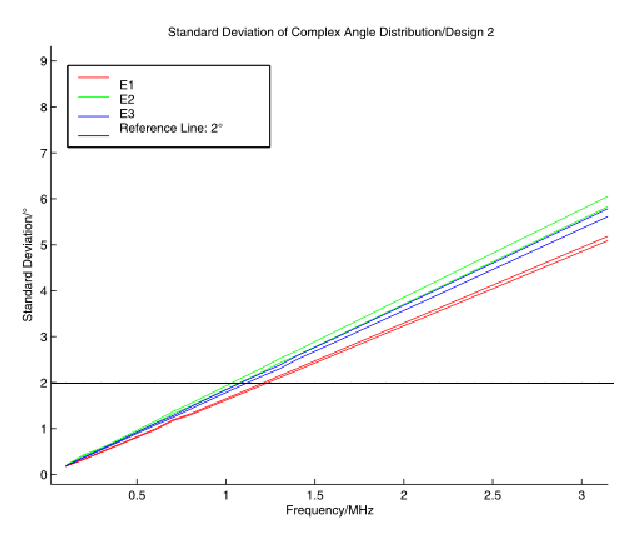
\includegraphics[width=12cm]{VirtualSigma1D2_caps.eps}\\
\caption{Standard deviation of the length, spacecraft A (full line) and B (dashed line)/capacitances Included} \label{fig_VirtualSigma1_D2_caps}
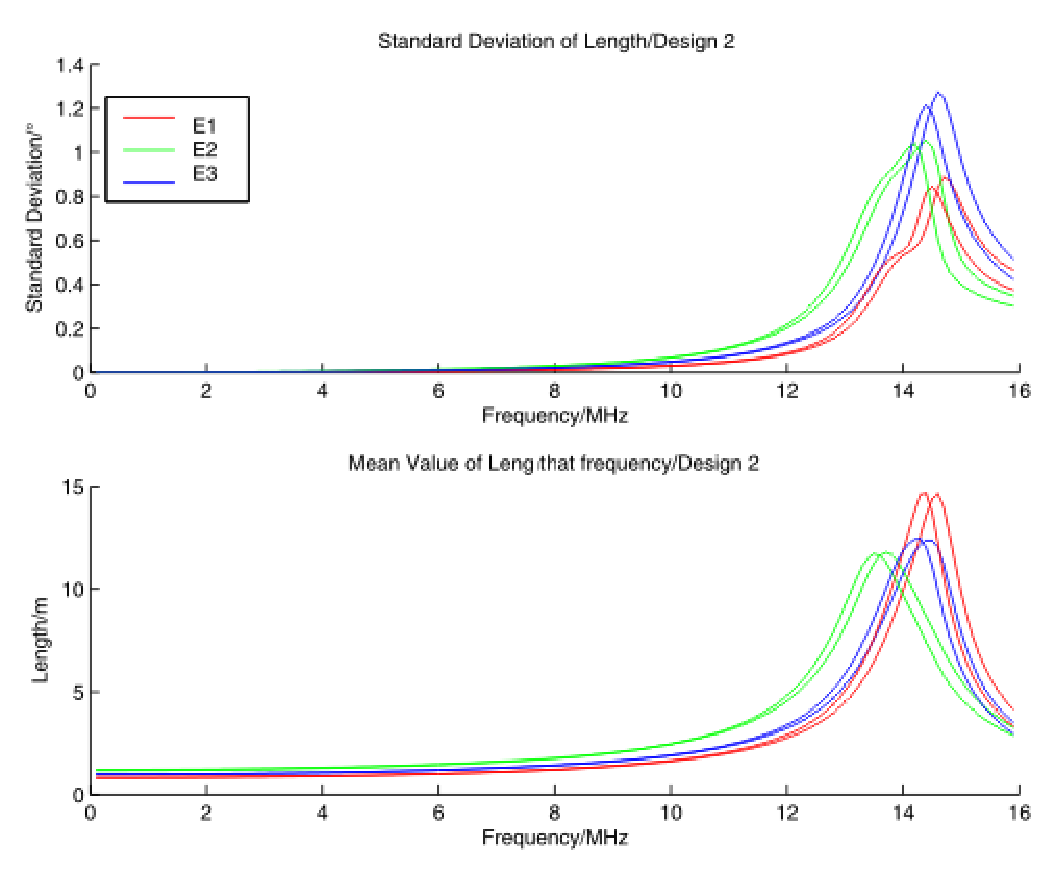
\includegraphics[width=12cm]{VirtualSigma2D2_caps.eps} \\
\caption{Complex standard deviation of the angular distribution, spacecraft A (full line) and B (dashed line)/capacitances included} \label{fig_VirtualSigma2_D2_caps}
\end{center}
\end{figure}

\subsection{The Covariance Matrix}
\paragraph*{}
When performing direction finding, it is useful to know the covariance matrix. We have written a matlab routine to compute the matrix. The formula for the elements of the matrix is

\begin{equation}\label{covariance}
    \sigma_{u,v}=\frac{1}{N-1}\sum_{i=1}^N(u_i-\bar{u})(v_i-\bar{v})
\end{equation}

\paragraph*{}
where $u_i$ and $v_i$ are the two observables. The diagonal elements are the variances and the other elements are the covariance that describe the interaction of the parameters. One would expect the variances to be larger than the covariances, which is reflected in the actual matrix below. The order of the parameters is\\
 $h_{eff}(E1), h_{eff}(E2), h_{eff}(E3), \xi(E1), \xi(E2),\xi(E3),\zeta(E1), \zeta(E2), \zeta(E3)$ and the units used are meter for the first three parameters and degree for the remaining 6. For frequencies of 500kHz and 1MHz, the results are tabulated in (\ref{cov_500kHz}) and (\ref{cov_1MHz}) for spacecraft A, and in (\ref{cov_500kHz_B}) and (\ref{cov_1MHz_B}) for spacecraft B.

\tiny
\begin{equation}\label{cov_500kHz}
10^{-9}\cdot \left(
\begin{array}{ccccccccc}
  \textbf{8.336} & -6.114 & -7.406 & -141.1 & 73.42 & -188.0 & -7.367 & -70.45 & -56.56 \\
-6.114 & \textbf{43.39} & -6.752 & -130.5 & -186.2 & 116.8 & -17.53 & 371.1 & -74.63 \\
-7.406 & -6.752 & \textbf{21.66} & 246.9 & -71.09 & 365.2 & -39.00 & -78.78 & 121.5 \\
 -141.2 & -130.5 & 246.29 & \textbf{4110} & -675.0 & 4056 & 207.3 & -836.4 & 1955 \\
 73.42 & -186.2 & -71.09 & -675.0 & \textbf{1307} & -2370 & 186.3 & -1554 & -294.9 \\
 -188.1 & 116.8 & 365.2 & 4056 & -2370 & \textbf{7556} & -818.3 & 673.2 & 1835 \\
 -7.367 & -17.53 & -39.00 & 207.3 & 186.3 & -818.3 & \textbf{526.7} & 172.2 & 192.1 \\
 -70.45 & 371.2 & -78.78 & -836.4 & -1554 & 673.2 & 172.2 & \textbf{3414} & -506.3 \\
 -56.56 & -74.64 & 121.5 & 1955 & -294.9 & 1835 & 192.1 & -506.3 & \textbf{1063} \\
\end{array}%
\right)
\end{equation}
\normalsize


\tiny
\begin{equation}\label{cov_1MHz}
10^{-7} \cdot \left(
\begin{array}{ccccccccc}
\textbf{1.343} & -.9867 & -1.192 & -22.50 & 11.93 & -30.54 & -1.020 & -11.42 & -8.983 \\
 -.9867 & \textbf{6.982} & -1.083 & -21.21 & -30.34 & 18.95 & -2.907 & 59.78 & -12.36 \\
 -1.192 & -1.083 & \textbf{3.491} & 39.44 & -11.57 & 59.07 & -6.382 & -12.51 & 19.55 \\
 -22.50 & -21.21 & 39.44 & \textbf{655.9} & -107.5 & 649.7 & 32.04 & -135.2 & 314.8 \\
 11.93 & -30.34 & -11.57 & -107.5 & \textbf{214.7} & -387.0 & 31.61 & -253.8 & -45.59 \\
 -30.53 & 18.95 & 59.07 & 649.7 & -387.0 & \textbf{1230} & -137.3 & 112.2 & 292.5 \\
 -1.020 & -2.907 & -6.382 & 32.04 & 31.61 & -137.3 & \textbf{84.54} & 25.64 & 31.20 \\
 -11.42 & 59.78 & -12.51 & -135.7 & -253.8 & 112.2 & 25.64 & \textbf{549.4} & -84.16 \\
 -8.983 & -12.36 & 19.55 & 314.8 & -45.59 & 292.5 & 31.20 & -84.16 & \textbf{171.6} \\
\end{array}%
\right)
\end{equation}
\normalsize


\tiny
\begin{equation}\label{cov_500kHz_B}
10^{-9}\cdot \left(
\begin{array}{ccccccccc}
 \textbf{9.334} & -6.884 & -8.201 & -135.0 & 76.76 & -189.4 & 1.641 & -74.17 & -57.16 \\
 -6.884& \textbf{46.80} & -7.603 & -132.0 & -186.7 & 116.3 & -30.78 & 387.1 & -84.76 \\
 -8.201 & -7.603 & \textbf{23.80} & 241.1 & -71.71 & 358.8 & -44.41 & -85.56 & 127.3 \\
 -135.0 & -132.0 & 241.1 & \textbf{3500} & -592.6 & 3533 & 73.09 & -881.2 & 1790 \\
 76.76 & -186.7 & -71.71 & -592.6 & \textbf{1228} & -2182 & 26.52 & -1501 & -252.3 \\
 -189.4 & 116.3 & 358.8 & 3533 & -2182 & \textbf{6705} & -900.10 & 648.2 & 1694 \\
 1.641& -30.78 & -44.41 & 73.09 & 265.2 & -900.1 & \textbf{478.2} & 22.78 & 132.2 \\
 -74.17 & 387.14 & -85.56 & -881.2& -150.2 & 648.3 & 22.78 & \textbf{3419} & -598.0 \\
 -57.16 & -84.76 & 127.3& 1790 & -252.3 & 1694 & 132.2 & -598.0 & \textbf{1035} \\
\end{array}%
\right)
\end{equation}
\normalsize


\tiny
\begin{equation}\label{cov_1MHz_B}
10^{-7} \cdot \left(
\begin{array}{ccccccccc}
\textbf{1.504} & -1.110 & -1.319 & -21.53 & 12.47 & -30.74 & .4189 & -12.01 & -9.079 \\
 -1.110 & \textbf{7.530} & -1.220 & -21.46 & -30.39 & 18.87 & -5.031 & 62.34 & -13.98 \\
 -1.319 & -1.220 & \textbf{3.833} & 38.63 & -11.66 & 58.02 & -7.247 & -13.61 & 20.48 \\
 -21.56 & -21.46 & 38.63 & \textbf{559.4} & -94.24 & 566.1 & 11.05 & -142.6 & 288.4 \\
 12.47 & -30.39 & -11.66 & -94.24 & \textbf{201.5} & -356.2 & 44.28 & -245.1 & -38.87\\
 -30.74 & 18.87 & 58.02 & 566.1 & -356.2 & \textbf{1091} & -150.0 & 107.7 & 270.2 \\
 .4189 & -5.031 & -7.247 & 11.07 & 44.28 & -149.8 & \textbf{77.16} & 1.853 & 21.74 \\
 -12.01 & 62.34 & -13.61 & -142.6 & -245.1 & 107.7 & 1.853 & \textbf{550.2} & -98.77 \\
 -9.079 & -13.98 & 20.48 & 288.7 & -38.87 & 270.20 & 21.74 & -98.77 & \textbf{167.1} \\
\end{array}%
\right)
\end{equation}
\normalsize


\paragraph*{}
The variances and covariances are rather small at low frequencies. Further research shows that they suddenly explode at about 12MHz. At 16MHz the variances of the angles have an order of magnitude of 30-40 degrees.

\subsection{Variation of the effective length vectors with frequency at fixed direction}
\paragraph*{}
The radiation, the spacecraft is going to measure, will have direction of arrival roughly
from the sun, which is located opposite to the boom (positive
x-axis). Therefore it is useful to compute the geometry of the effective length vectors for this direction in detail. Diagrams \ref{fig_Heff_length_abs_caps_D2} - \ref{fig_Heff_length_imag_caps_D2} show the length of the effective length vectors as a function of
frequency. Again, the result for STEREO A is plotted in solid lines while the results for STEREO B is plotted in dashed lines. The strange behavior in the second graph between 13 and 14MHz can be explained when realizing that the absolute values of the real parts are plotted. So the real part of the antenna E2 even changes its direction at this resonance frequency.

\newpage
\begin{figure}
\begin{center}
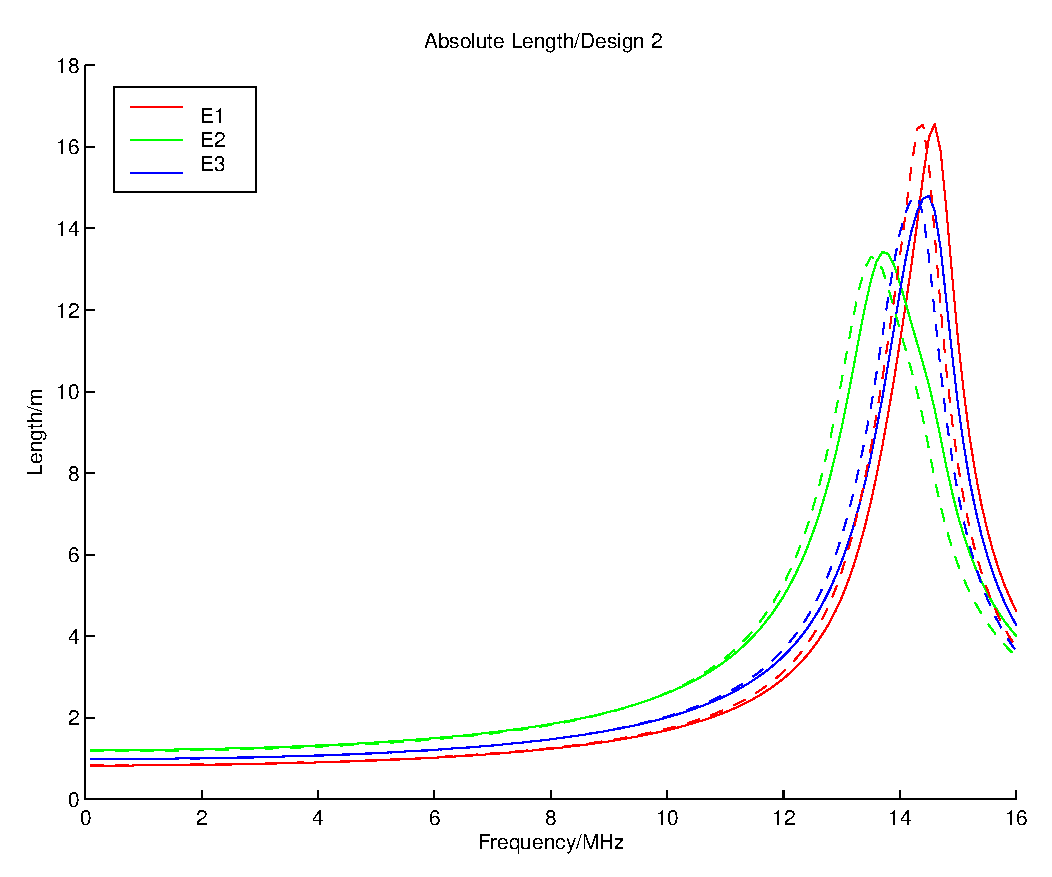
\includegraphics[scale=0.45]{HeffLengthAbsD2_caps.eps}\\
\caption{The absolute length of the electric antennas of the  design 2 model/ Capacitances included} \label{fig_Heff_length_abs_caps_D2}
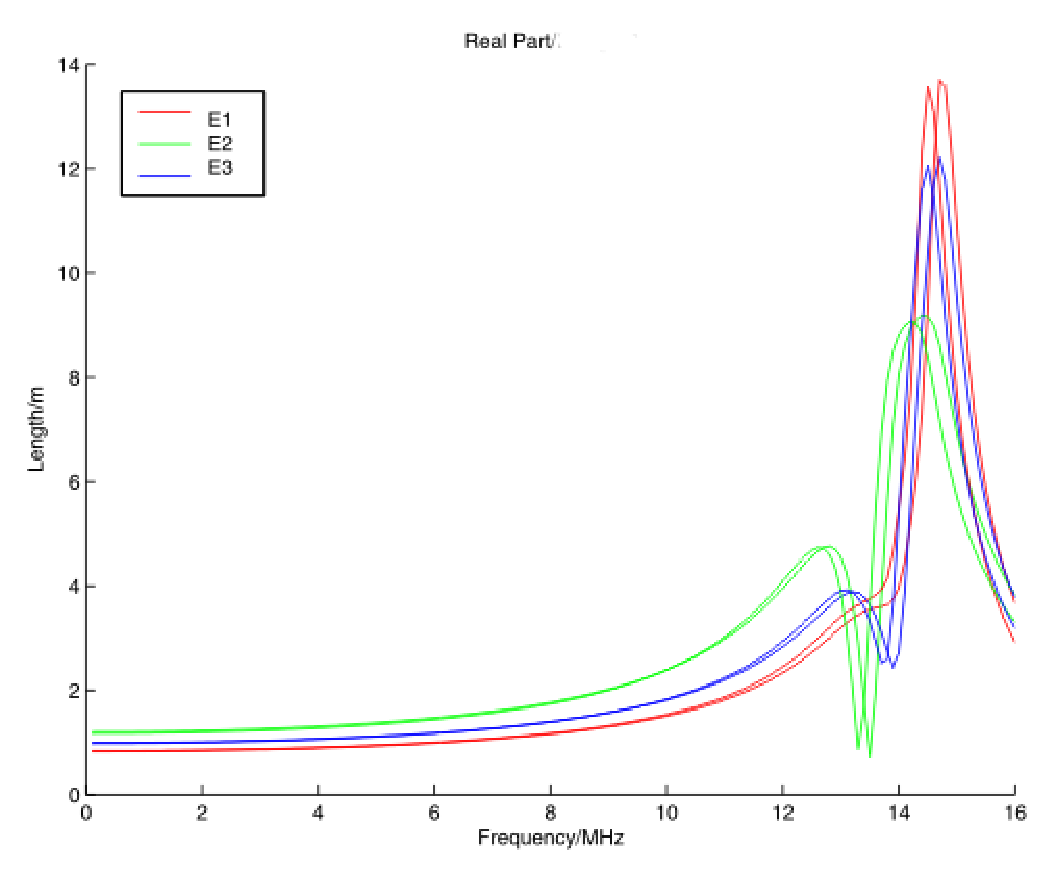
\includegraphics[scale=0.45]{HeffLengthRealD2_caps.eps} \\
\caption{The length of the real parts of the electric antennas of the  design 2 model/Capacitances included} \label{fig_Heff_length_real_caps_D2}
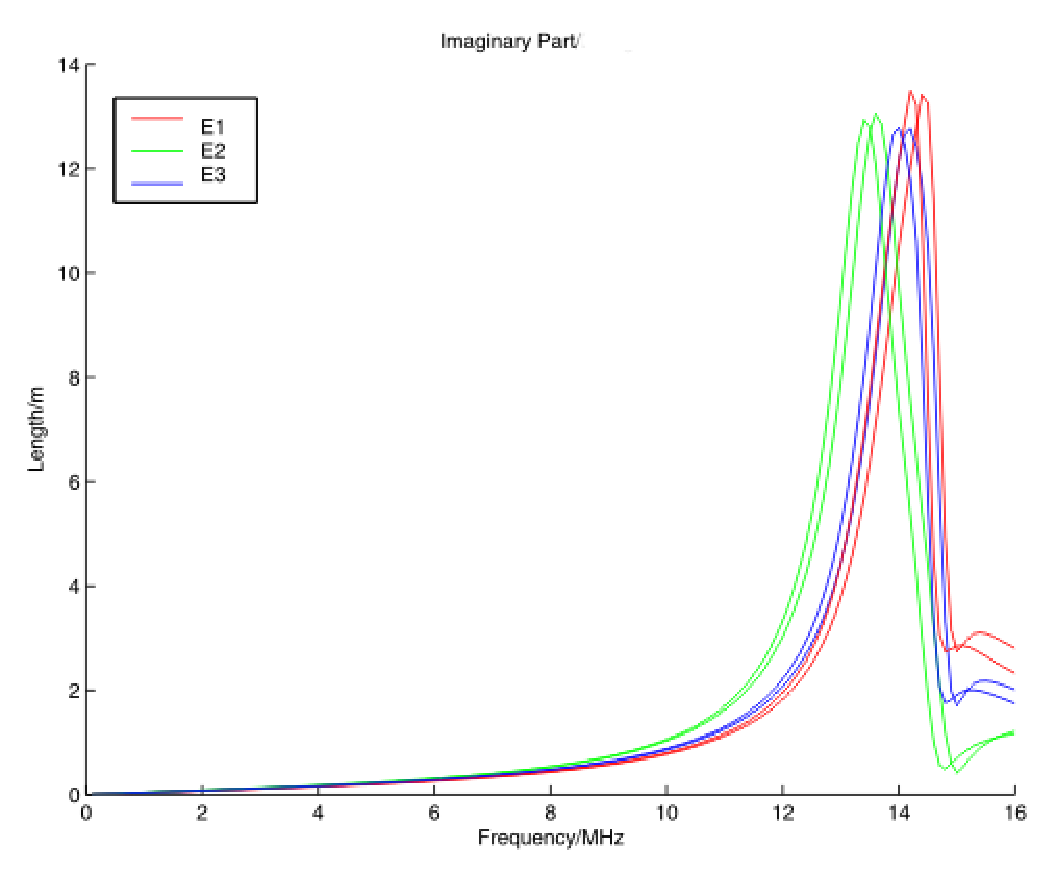
\includegraphics[scale=0.45]{HeffLengthImagD2_caps.eps} \\
\caption{The length of the imaginary parts of the electric antennas of the  design 2 model/Capacitances included} \label{fig_Heff_length_imag_caps_D2}
\end{center}
\end{figure}

\paragraph*{}
As one can see, the resonances at 14MHz change drastically the
effective lengths of the antennas. The imaginary part of $\mathbf{h_{eff}}$ vanishes as the
frequency goes to zero while the real part converges to the quasistatic limit. The source of the kink of the real part between 13 and 14MHz is not yet clear.
\\

\subsection{Variation of the effective length vectors with different HGA angles}
\paragraph*{}
Similar to the visualization of the dependance of the effective length vectors of the direction of the radiation, their dependance of the position of the HGA dish can be shown. Like before, the frequency is color coded, but this time I only present the results for spacecraft A. The plots for spacecraft B are similar.


\paragraph*{}
Figure \ref{fig_heff_dist_HGA_D2_A_Z_View_caps} shows the color coded plot that show the variability of the electric antennas due to the turnable HGA dish. It seems that the different angles of the HGA dish has greart influence upon the receiving properties of the stacer antennas in a frequency range up to 14MHz. Figures \ref{fig_heff_dist_HGA_D2_A_X_View_caps}-\ref{fig_heff_dist_HGA_D2_A_Z_View_caps2} are created with a frequency range up to 13MHz which is short below the resonance frequency. The erratic behavior vanished.\\

\begin{figure}
\begin{center}
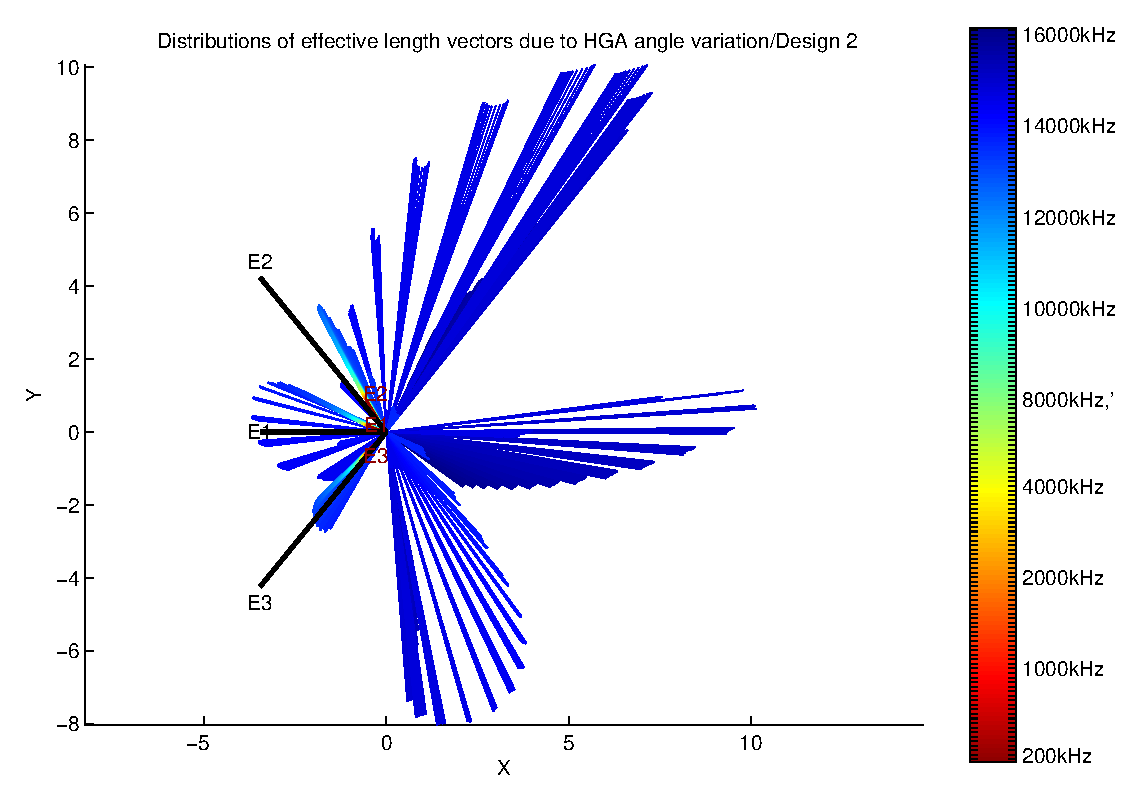
\includegraphics[width=12cm]{HeffVerteilungHGAD2-ZView_caps.eps} \\
\caption{The spatial distribution of the real parts of the effective length vectors of the design 2 model, capacitances included/Z View}\label{fig_heff_dist_HGA_D2_A_Z_View_caps}
\end{center}
\end{figure}


\begin{figure}
\begin{center}
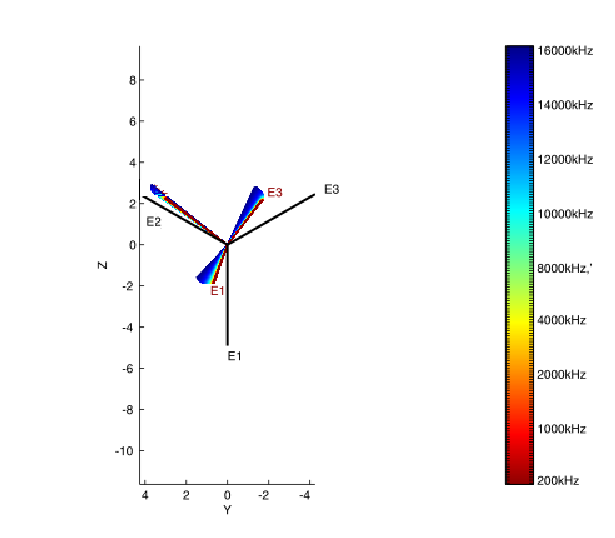
\includegraphics[width=12cm]{HeffVerteilungHGAD2-XView_caps.eps}\\
\caption{The spatial distribution of the real parts of the effective length vectors of the design 2 model, capacitances included/X View}\label{fig_heff_dist_HGA_D2_A_X_View_caps}
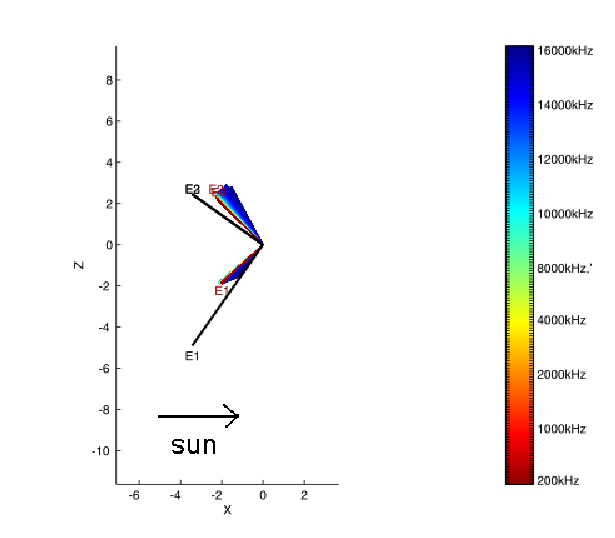
\includegraphics[width=12cm]{HeffVerteilungHGAD2-YView_caps.eps} \\
\caption{The spatial distribution of the real parts of the effective length vectors of the design 2 model, capacitances included/Y View}\label{fig_heff_dist_HGA_D2_A_Y_View_caps}
\end{center}
\end{figure}

\begin{figure}
\begin{center}
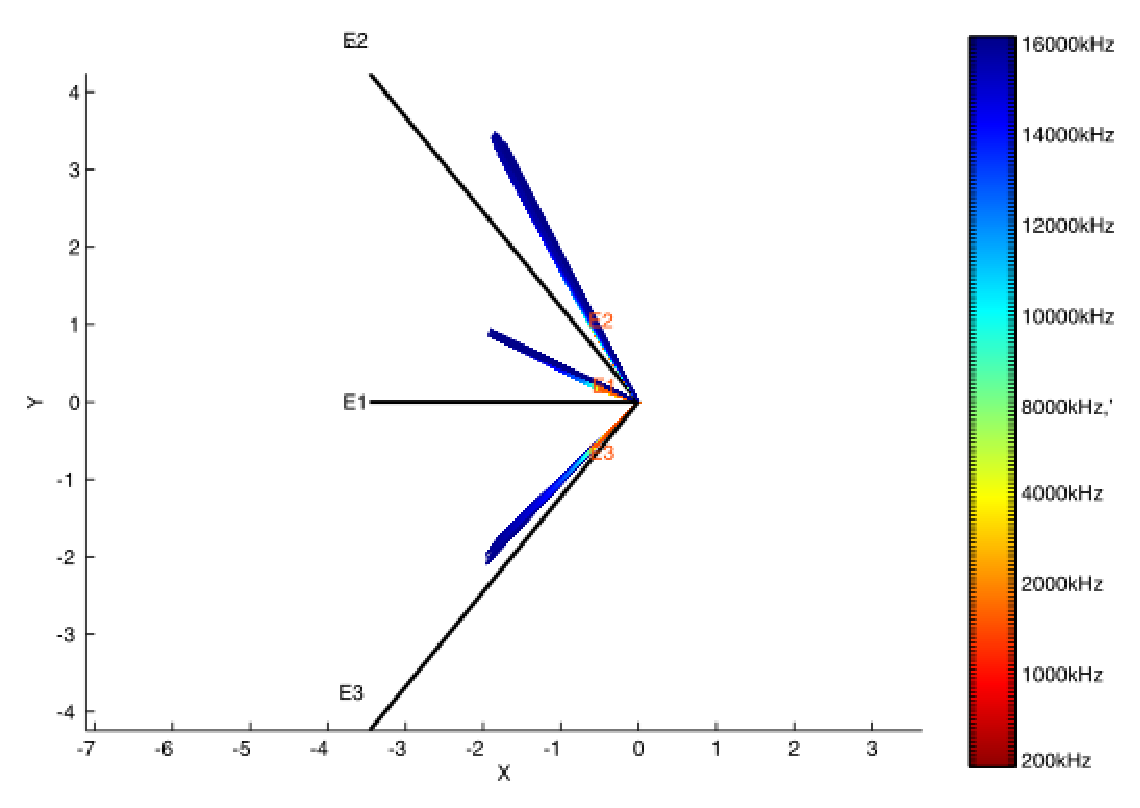
\includegraphics[width=12cm]{HeffVerteilungHGAD2-ZView_caps2.eps} \\
\caption{The spatial distribution of the real parts of the effective length vectors of the design 2 model, capacitances included/Z View}\label{fig_heff_dist_HGA_D2_A_Z_View_caps2}
\end{center}
\end{figure}


\begin{table}
\centering
\caption{Variation of E1 due to HGA angle variation with base capacitances included}\label{tab_e1_var}
\begin{tabular}{|c|c|c|c|}
  \hline
HGA angle & $\sigma_{h_{eff}}$ & $\sigma_{\zeta}$ & $\sigma_{\xi}$ \\
\hline
-90 & 0.83 & 128.5 & 14.5 \\
-80 & 0.83 & 128.5 & 14.5 \\
-70 & 0.83 & 128.5 & 14.4 \\
-60 & 0.83 & 128.4 & 14.5 \\
-50 & 0.83 & 128.4 & 14.5 \\
-40 & 0.83 & 128.4 & 14.5 \\
-30 & 0.83 & 128.4 & 14.2 \\
-20 & 0.83 & 128.3 & 14.7 \\
-10 & 0.83 & 128.3 & 14.9 \\
0 & 0.83 & 128.2 & 15.0 \\
10 & 0.83 & 128.1 & 15.0 \\
20 & 0.83 & 128.0 & 15.1 \\
30 & 0.83 & 127.8 & 15.1 \\
40 & 0.83 & 127.7 & 15.2 \\
50 & 0.83 & 127.7 & 15.2 \\
60 & 0.83 & 127.6 & 15.3 \\
70 & 0.83 & 127.6 & 15.3 \\
80 & 0.83 & 127.7 & 15.4 \\
90 & 0.83 & 127.7 & 15.4 \\
\hline\end{tabular}
\end{table}

\newpage
\begin{table}
\centering
\caption{Variation of E2 due to HGA angle variation with base capacitances included}\label{tab_e12var}
\begin{tabular}{|c|c|c|c|}
  \hline
% after \\: \hline or \cline{col1-col2} \cline{col3-col4} ...
HGA angle & $\sigma_{h_{eff}}$ & $\sigma_{\zeta}$ & $\sigma_{\xi}$ \\
\hline
-90 & 1.20 & 117.4 & 125.9 \\
-80 & 1.20 & 117.4 & 125.9 \\
-70 & 1.20 & 117.4 & 125.8 \\
-60 & 1.20 & 117.4 & 125.8 \\
-50 & 1.20 & 117.3 & 125.8 \\
-40 & 1.20 & 117.3 & 125.8 \\
-30 & 1.20 & 117.3 & 125.9 \\
-20 & 1.20 & 117.2 & 125.8 \\
-10 & 1.20 & 117.2 & 125.7 \\
0 & 1.21 & 117.1 & 125.8 \\
10 & 1.21 & 117.0 & 125.7 \\
20 & 1.20 & 117.0 & 125.6 \\
30 & 1.20 & 116.9 & 125.4 \\
40 & 1.20 & 116.9 & 125.4 \\
50 & 1.20 & 116.8 & 125.3 \\
60 & 1.20 & 116.8 & 125.3 \\
70 & 1.20 & 116.8 & 125.3 \\
80 & 1.20 & 116.8 & 125.4 \\
90 & 1.21 & 116.8 & 125.5 \\
\hline\end{tabular}
\end{table}

\begin{table}
\centering
\caption{Variation of E3 due to HGA angle variation with base capacitances included}\label{tab_e3_var}
\begin{tabular}{|c|c|c|c|}
  \hline
% after \\: \hline or \cline{col1-col2} \cline{col3-col4} ...
HGA angle & $\sigma_{h_{eff}}$ & $\sigma_{\zeta}$ & $\sigma_{\xi}$ \\
\hline
-90 & 1.00 & 123.7 & -136.7 \\
-80 & 1.00 & 123.7 & -136.6\\
-70 & 0.99 & 123.7 & -136.6\\
-60 & 0.99 & 123.7 & -136.6\\
-50 & 0.99 & 123.7 & -136.6\\
-40 & 0.99 & 123.7 & -136.7\\
-30 & 0.99 & 123.4 & -136.5\\
-20 & 0.99 & 123.6 & -136.9\\
-10 & 0.99 & 123.6 & -137.0\\
0 & 0.99 & 123.5 &  -137.2\\
10 & 0.98 & 123.5 & -137.3\\
20 & 0.98 & 123.5 & -137.3\\
30 & 0.97 & 123.6 & -137.4\\
40 & 0.96 & 123.6 & -137.4 \\
50 & 0.96 & 123.6 & -137.4\\
60 & 0.96 & 123.5 & -137.5 \\
70 & 0.96 & 123.5 & -137.5 \\
80 & 0.96 & 123.4 & -137.6 \\
90 & 0.97 & 123.3 & -137.7 \\
\hline\end{tabular}\\
\end{table}
\paragraph*{}
Figures \ref{fig_VirtualSigma1_HGA_D2_caps} and \ref{fig_VirtualSigma2_HGA_D2_caps} show quantitatively the influence of the HGA angle.

\begin{figure}[h]
\begin{center}
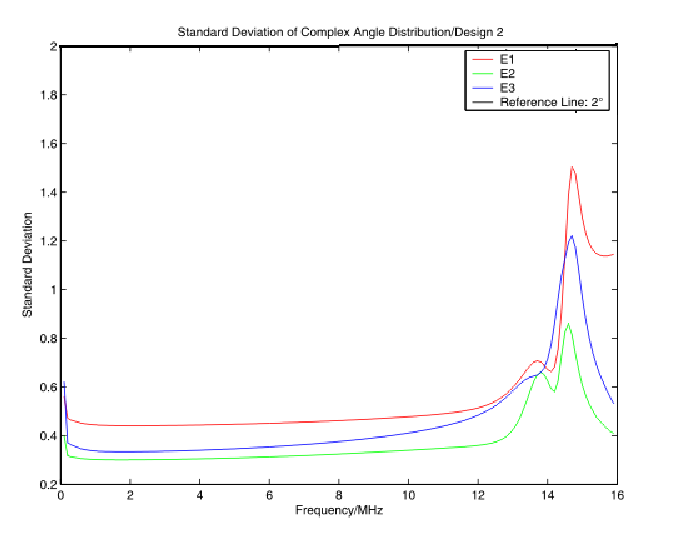
\includegraphics[width=12cm]{VirtualSigma1D2HGA_caps.eps}\\
\caption{Complex standard deviation of the angular distribution due to HGA angle variation, capacitances included} \label{fig_VirtualSigma1_HGA_D2_caps}
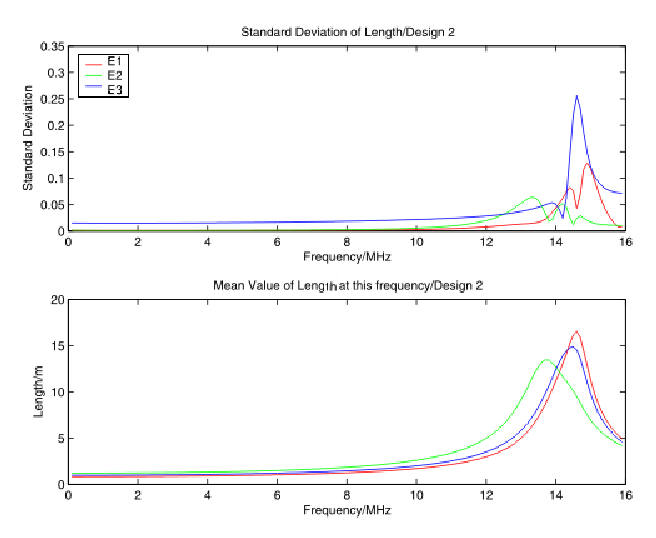
\includegraphics[width=12cm]{VirtualSigma2D2HGA_caps.eps} \\
\caption{Standard deviation of the length due to HGA angle variation, capacitances included} \label{fig_VirtualSigma2_HGA_D2_caps}
\end{center}
\end{figure}

\newpage

\subsection{The Impedances and Admittances}
\paragraph*{}
On the plots of the admittances, the first resonances can be seen
at a frequency of approximately 14MHz. A resonance exists, if the
effective length of the antenna is equal to $\frac{1}{4}$ of the
wavelength of the incident radiation. In the case of the
spacecraft, the length of the distance between the tip of the
antenna and the furthest point on the spacecraft has to be taken.
In case of STEREO, the longest distances are between the boom and
the antennas and between the edge of the opposite solar panel and
the tip of the antennas. The wavelength of an
electromagnetic wave at 12MHz is 25 meters, so $\frac{\lambda}{4}$
is 6.25m. Hence we would expect two resonances in
the frequency range around 12MHz, but the inclusion of the capacitances of the receiver, the cable and the base capacitances of the antennas has the effect to increase the resonance frequency, which is the reason that we can see the first resonance at 12MHz. Since the capacitances are parallel to the antenna capacitances, both can be added. To get the overall impedance, the reciprocal values have to be added, while the admittances have simply to be added. The two resonances can partly be seen on the plot of the admittances, but in general they are too close together to be resolved.


\paragraph*{}
 Plots of the resultant impedances are shown in Figures \ref{fig_Impedance1_D2_caps} - \ref{fig_Impedance2_D2B_caps}, plots of the resultant admittances in Figures \ref{fig_Admittance1_D2_caps} - \ref{fig_Admittance2_D2B_caps}. While in the first plot, the real and imaginary parts are plotted as a function of frequency, the imaginary part is plotted as a function of the real part in the lower graph. The resonance occurs when the imaginary part of the impedance is zero. Then the antenna is pure resistive.

\begin{figure}
\begin{center}
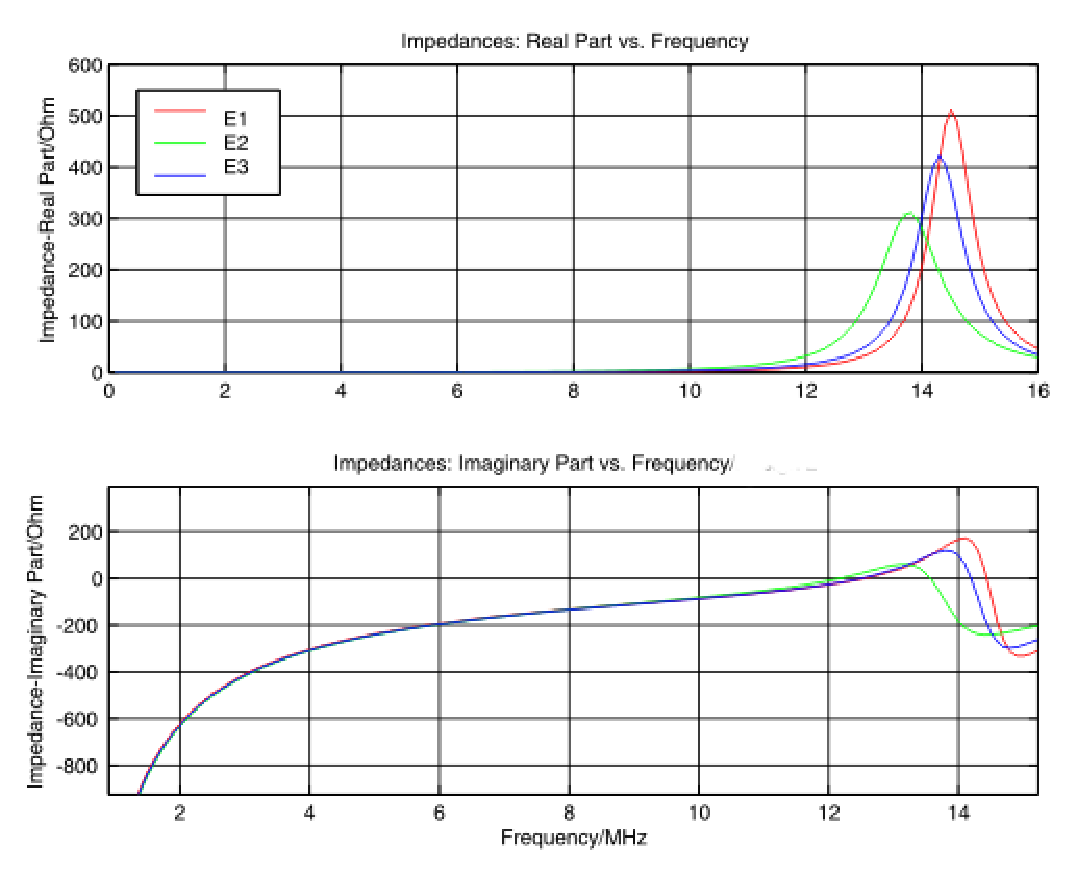
\includegraphics[scale=0.65]{ImpedancesD21_caps.eps}\\
\caption{Impedances of Design 2, spacecraft A, capacitances included} \label{fig_Impedance1_D2_caps}
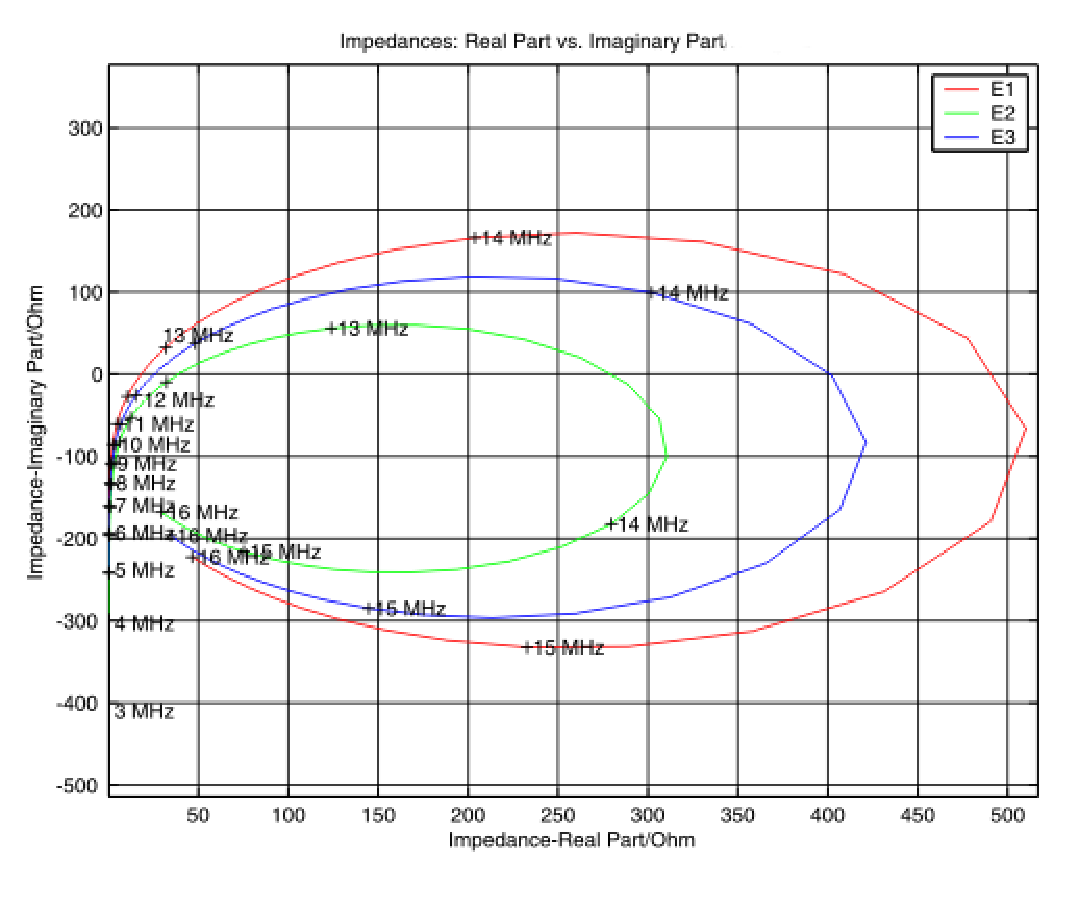
\includegraphics[scale=0.65]{ImpedancesD22_caps.eps} \\
\caption{Impedances of Design 2, spacecraft A, capacitances included} \label{fig_Impedance2_D2_caps}
\end{center}
\end{figure}
\begin{figure}
\begin{center}
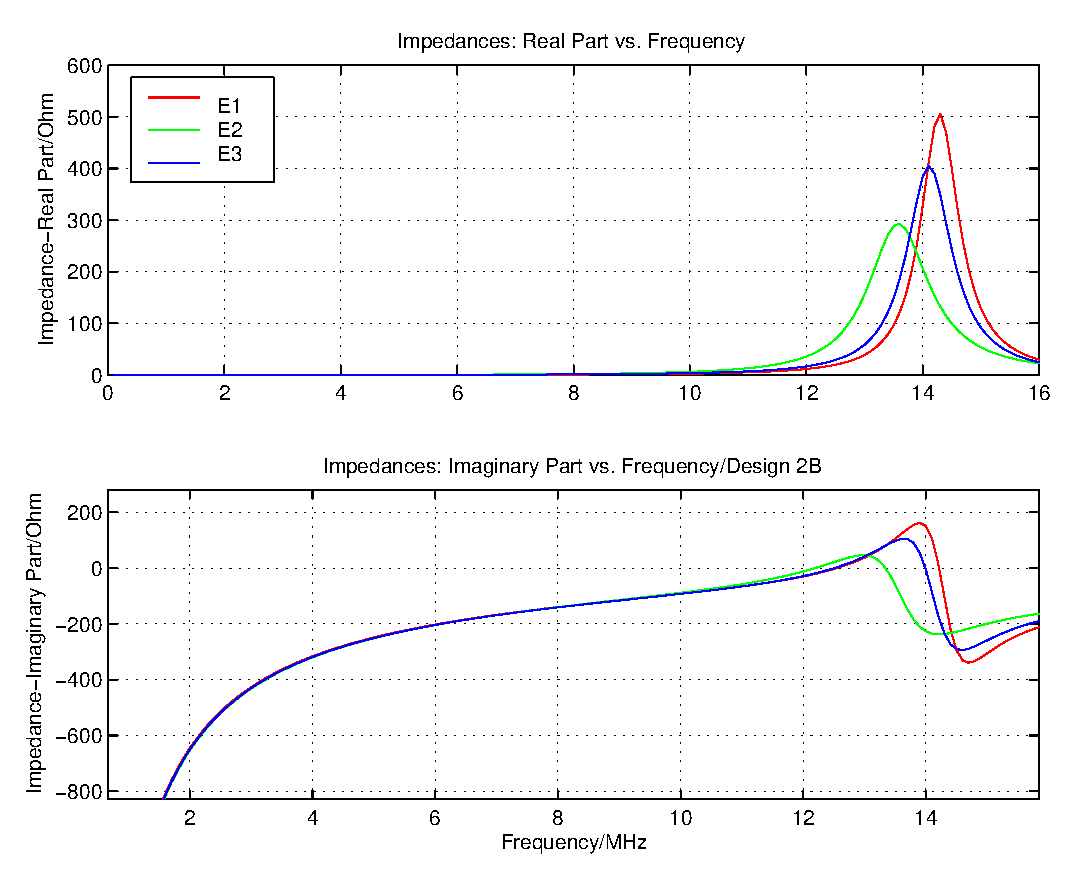
\includegraphics[scale=0.65]{ImpedancesD2B1_caps.eps}\\
\caption{Impedances of Design 2, spacecraft B, capacitances included} \label{fig_Impedance1_D2B_caps}
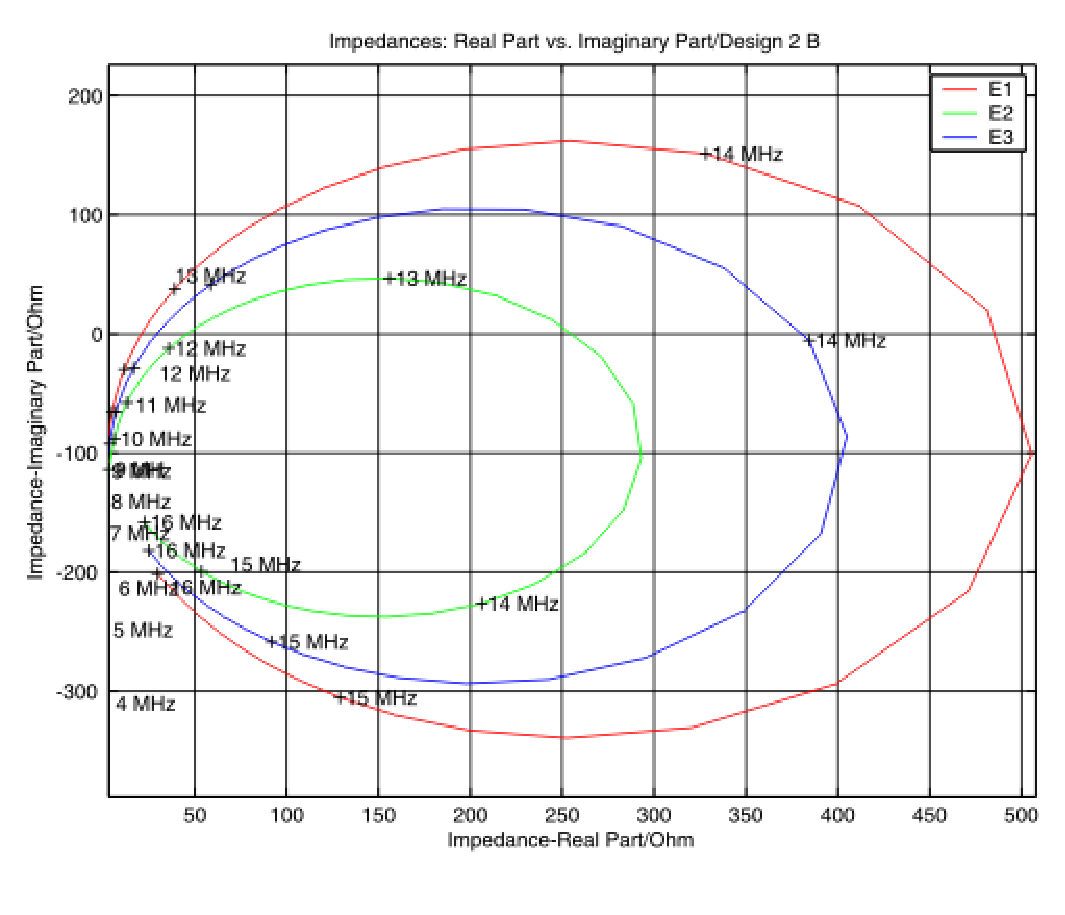
\includegraphics[scale=0.65]{ImpedancesD2B2_caps.eps} \\
\caption{Impedances of Design 2, spacecraft B, capacitances included} \label{fig_Impedance2_D2B_caps}
\end{center}
\end{figure}
\begin{figure}
\begin{center}
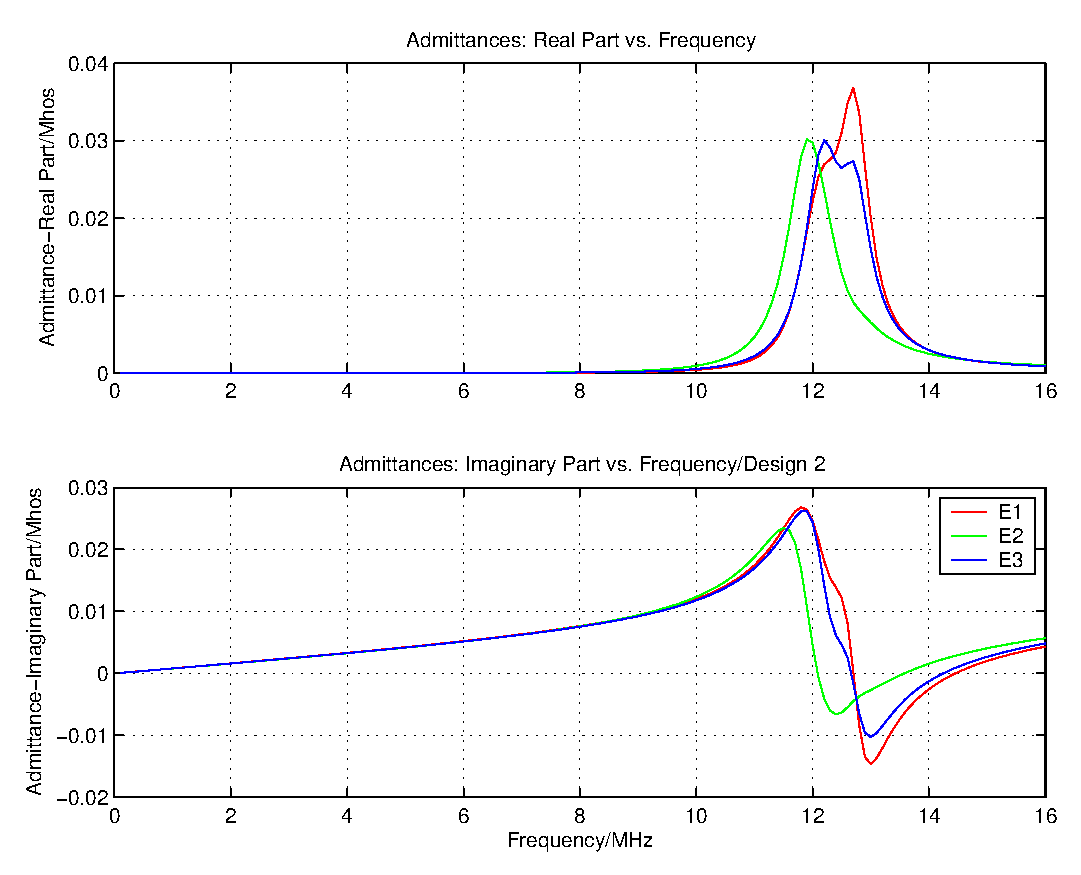
\includegraphics[scale=0.65]{AdmittancesD21_caps.eps}\\
\caption{Admittances of Design 2, spacecraft A, capacitances included} \label{fig_Admittance1_D2_caps}
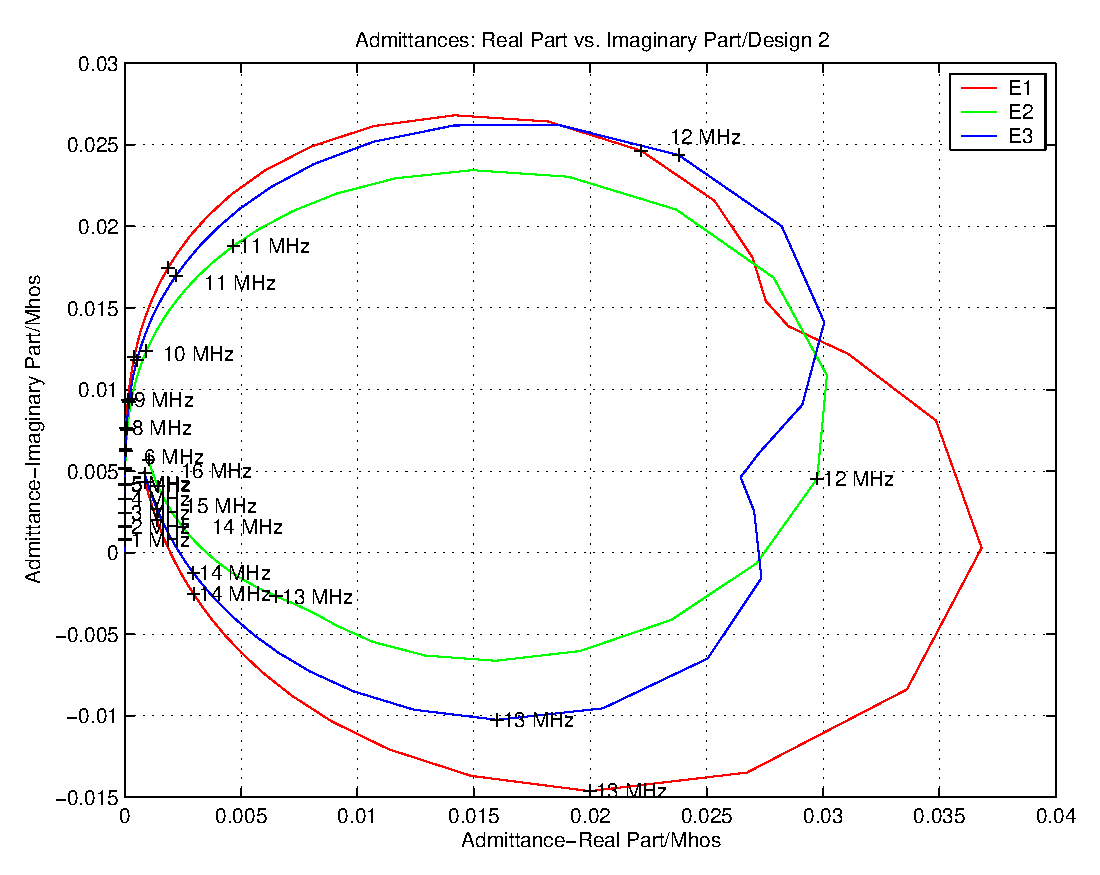
\includegraphics[scale=0.65]{AdmittancesD22_caps.eps} \\
\caption{Admittances of Design 2, spacecraft A, capacitances included} \label{fig_Admittance2_D2_caps}
\end{center}
\end{figure}
\begin{figure}
\begin{center}
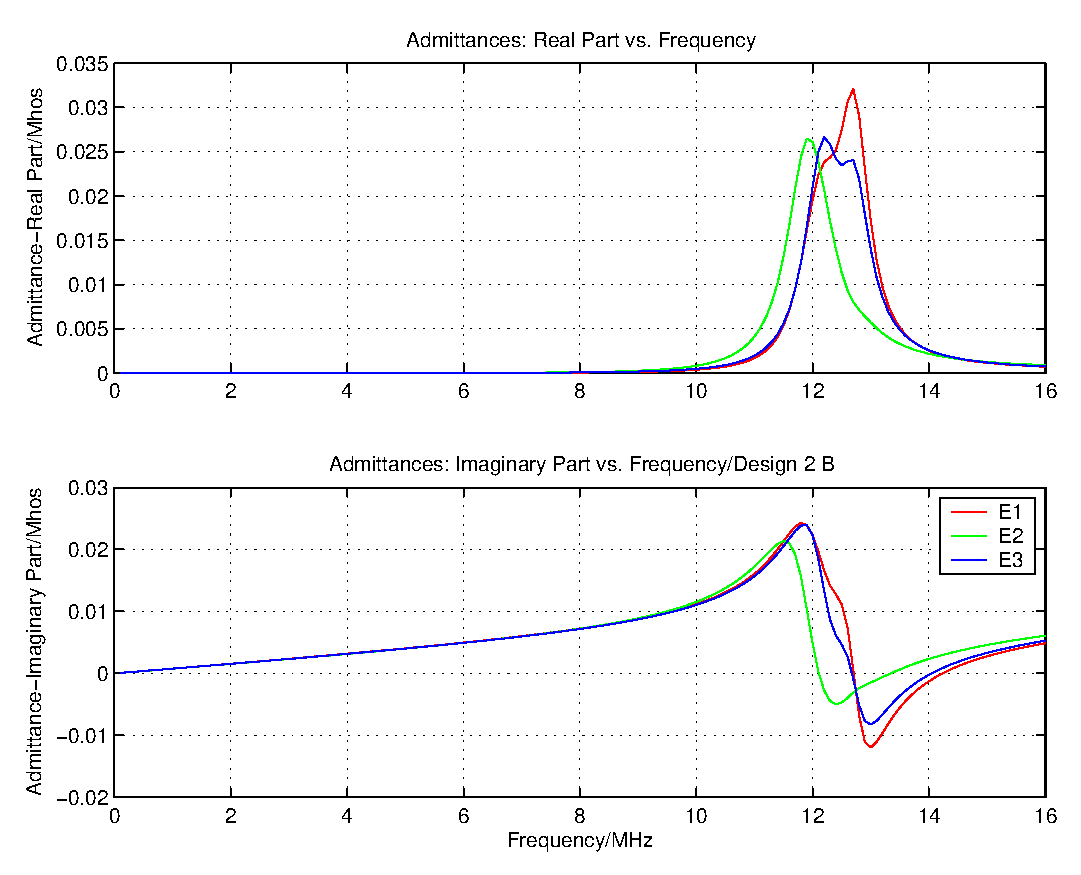
\includegraphics[scale=0.65]{AdmittancesD2B1_caps.eps}\\
\caption{Admittances of Design 2, spacecraft B, capacitances included} \label{fig_Admittance1_D2B_caps}
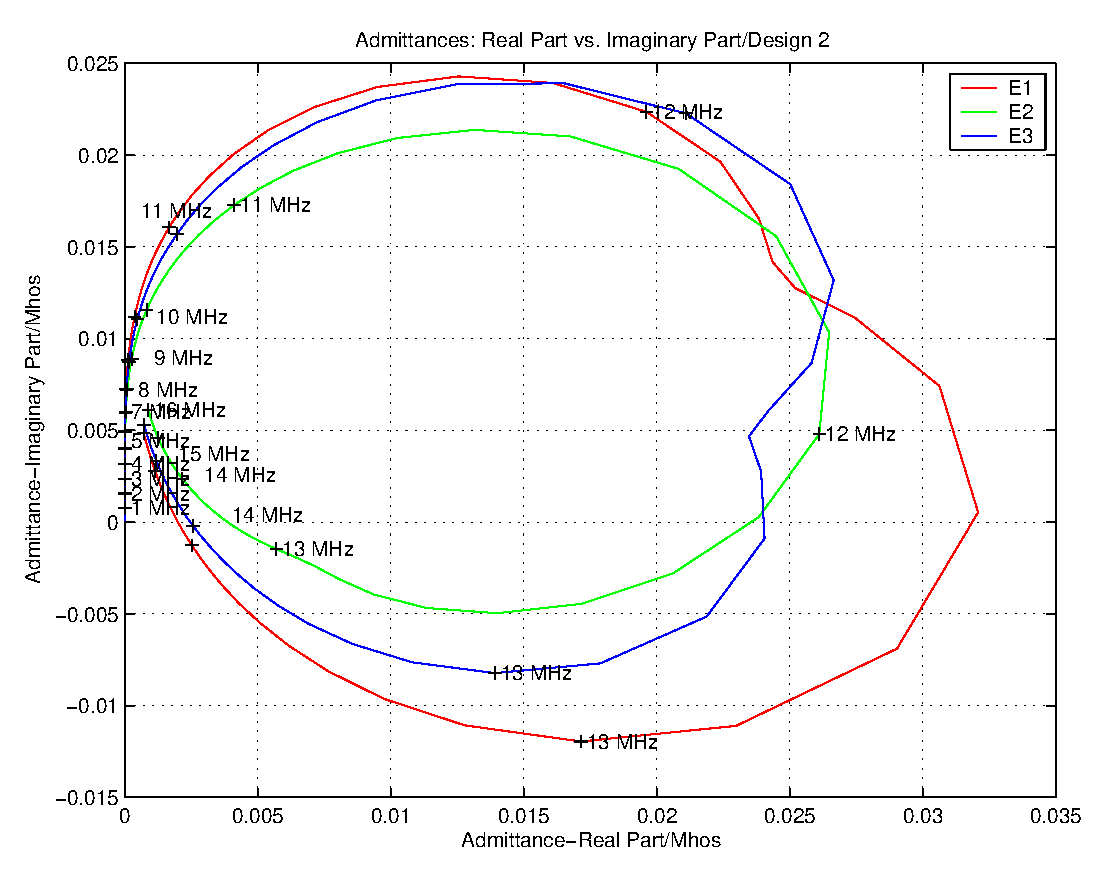
\includegraphics[scale=0.65]{AdmittancesD2B2_caps.eps} \\
\caption{Admittances of Design 2, spacecraft B, capacitances included} \label{fig_Admittance2_D2B_caps}
\end{center}
\end{figure}
\paragraph*{}
The resonances can clearly be seen in the plots. The inclusion of the capacitances has the effect of increasing the imaginary part of the admittances, which, in turn, lowers the resonance frequency.


\chapter{\textbf{Conclusions}}
\paragraph*{}
Electromagnetic waves are an important tool in space research. Some major aspects are covered in this Master Thesis. At first, the equations, describing the wave propagation through vacuum and through plasma were derived. Then the subject of transmitting and receiving electromagnetic radiation was treated in the chapter about antennas. In the fourth chapter, a method was developed to calculate the direction of the incident wave and the Stokes parameters, a procedure called direction finding. The method was already successfully used in preceding studies. Finally, the antenna properties and effective length vectors of two NASA spacecraft STEREO A and STEREO B, which will be launched in a few month, were calculated by numerical means. These calculations were part of an ASAP project.

\paragraph{}
A very important aspect, which was not covered here, is the influence of magnetized plasma on the antenna properties. Much research is needed in this area.

%\chapter{\textbf{References}}
\backmatter
\begin{thebibliography}{24}
\providecommand{\natexlab}[1]{#1}
\expandafter\ifx\csname urlstyle\endcsname\relax
  \providecommand{\doi}[1]{doi:\discretionary{}{}{}#1}\else
  \providecommand{\doi}{doi:\discretionary{}{}{}\begingroup
  \urlstyle{rm}\Url}\fi

\bibitem[{\textit{Burden and Faires}(1999)}]{burdenfaires}
Burden, R., and D.~Faires (1999), \textit{Numerical Analysis}, Brooks/Cole
  Publishing Company.

\bibitem[{\textit{Cecconi and Zarka}(2004)}]{cecconi04}
Cecconi, B., and P.~Zarka (2004), Direction finding and antenna calibration
  through analytical inversion of radio measurements performed using a system
  of 2 or 3 electric dipole wire antennas on a 3 axes stabelized spacecraft,
  \textit{Radio Sci./ in press}.

\bibitem[{\textit{Fischer et~al.}(2000)}]{toolbox}
Fischer, G., W.~Macher, and H.~Rucker (2000), A matlab toolbox for calculating
  asap-wire-grid-models of antennas, \textit{Technical Report of the Space
  Research Institute/Austrian Academy of Science}, \textit{Nr. 121}.

\bibitem[{\textit{Fischer et~al.}(2001)}]{cassini}
Fischer, G., W.~Macher, H.~Rucker, H.~Ladreiter, and D.~Vogl (2001), Wire-grid
  modeling of Cassini spacecraft for the determination of effective antenna
  length vectors of the RPWS antennas, in \textit{Proc. Planetary Radio
  Emissions V}, edited by H.~Rucker, M.~Kaiser, and Y.~Leblanc, pp. 347--356,
  Austrian Academy of Sciences Press, Vienna.

\bibitem[{\textit{Fischer et~al.}(2003)}]{cassini2}
Fischer, G., W.~Macher, H.~Rucker, H.~Ladreiter, and D.~Vogl (2003), Reception
  properties of the Cassini/RPWS antennas from 1 to 16 mhz, poster at the
  EGS-AGU-EUG Joint Assembly, Nice.

\bibitem[{\textit{Grant and Phillips}(1999)}]{grant}
Grant, I.~S., and W.~R. Phillips (1999), \textit{Electromagnetism, Second
  Edition}, John Wiley \& Sons.

\bibitem[{\textit{Jackson}(1981)}]{jackson}
Jackson, J. (1981), \textit{Klassische Elektrodynamik}, de Gruyter.

\bibitem[{\textit{Ladreiter et~al.}(1995)}]{ladreiter_03}
Ladreiter, H., P.~Zarka, A.~Lecacheux, W.~Macher, H.~Rucker, R.~Manning,
  D.~Gurnett, and W.~Kurth (1995), Analysis of electromagnetic wave direction
  finding performed by spaceborne antennas using singular value decomposition
  techniques, \textit{Radio Sci.}, \textit{30}, 1699--1712.

\bibitem[{\textit{Leitinger}(2004)}]{leitinger}
Leitinger, R. (2004), Brechungsquotient fuer radiowellen in einem
  magneto-plasma.

\bibitem[{\textit{Macher}(1997)}]{macher_dipl}
Macher, W. (1997), Theorie effektiver hoehenvektoren von antennen mit anwendung
  auf das radio and plasma wave science experiment der Cassini raumsonde,
  Master's thesis, Technische Universit�t Graz.

\bibitem[{\textit{Macher and Vejda}(2003)}]{toolbox2}
Macher, W., and T.~Vejda (2003), Design of antenna grid structures. manual to
  the matlab toolbox, \textit{Technical Report of the Space Research
  Institute/Austrian Academy of Science}, \textit{Nr. 144}.

\bibitem[{\textit{Macher et~al.}(2002)}]{marsis}
Macher, W., B.~Schrausser, G.~Fischer, H.~Rucker, H.~Lammer, C.~Kolb, and
  G.~Kargl (2002), Analysis of sounding antennas of the mars-express marsis
  experiment, in \textit{Proc. 2nd European Workshop on Exo/Astrobiology},
  edited by H.~Sawaya-Lacoste, pp. 539--540, ESA Publications Division,
  Noordwijk, ESA SP-518.

\bibitem[{\textit{Macher et~al.}(2004)}]{marsis2}
Macher, W., H.~Rucker, G.~Fischer, and M.~Team (2004), Analysis of the marsis
  antenna system onboard mars express, poster at the EGU 1st General Assembly,
  Nice.

\bibitem[{\textit{Oswald et~al.}(2004)}]{antenna_report_1}
Oswald, T., W.~Macher, G.Fischer, and H.~Rucker (2004), First results of
  stereo/waves antenna calibration, \textit{Technical Report of the Space
  Research Institute/Austrian Academy of Science}, \textit{Nr. 160}.

\bibitem[{\textit{Oswald et~al.}(2005{\natexlab{a}})}]{antenna_report_2}
Oswald, T., W.~Macher, G.Fischer, and H.~Rucker (2005{\natexlab{a}}), Results
  of stereo/waves antenna calibration, using a refined spacecraft model (design
  2), \textit{Technical Report of the Space Research Institute/Austrian Academy
  of Science}, \textit{Nr. 167}.

\bibitem[{\textit{Oswald et~al.}(2005{\natexlab{b}})}]{DF}
Oswald, T., H.~Rucker, W.~Macher, G.Fischer, and U.~Taubenschuss
  (2005{\natexlab{b}}), Direction finding, \textit{Technical Report of the
  Space Research Institute/Austrian Academy of Science}, \textit{Nr. 168}.

\bibitem[{\textit{Press et~al.}(1999)}]{recipes}
Press, W., S.A.Teukolsky, W.T.Vetterling, and B.P.Flannery (1999),
  \textit{Numerical Recipes in C}, Cambridge University Press.

\bibitem[{\textit{Rucker et~al.}(1996)}]{rheometry}
Rucker, H., W.~Macher, R.~Manning, and H.~Ladreiter (1996), Cassini model
  rheometry, \textit{Radio Sci.}, \textit{31}(6), 1299--1311.

\bibitem[{\textit{Rucker et~al.}(2005)}]{ruckerundi05}
Rucker, H., W.~Macher, G.~Fischer, T.~Oswald, J.-L. Bougeret, M.~Kaiser, and
  K.~Goetz (2005), Analysis of spacecraft antenna systems: Implications for
  stereo/waves, \textit{Adv. Space Res. in press}.

\bibitem[{\textit{Rucker et~al.}(1997)}]{cassini3}
Rucker, H.~O., W.~Macher, and S.~Albrecht (1997), Experimental and theoretical
  investigations on the Cassini RPWS antennas, in \textit{Proc. Planetary Radio
  Emissions IV}, edited by H.~Rucker, S.~J. Bauer, and A.~Lecacheux, pp.
  327--337, Austrian Academy of Sciences Press Vienna.

\bibitem[{\textit{Staelin et~al.}(1994)}]{emwaves}
Staelin, D., A.~Morgenthaler, and J.Kong (1994), \textit{Electromagnetic
  Waves}, Prentice Hall.

\bibitem[{\textit{Taubenschuss}(2005)}]{uli1}
Taubenschuss, U. (2005), private Communication.

\bibitem[{\textit{Vogl et~al.}(2001)}]{vogl_01}
Vogl, D., H.~Ladreiter, P.~Zarka, H.~Rucker, W.~Macher, W.~S. Kurth,
  D.~Gurnett, and G.~Fischer (2001), First results on the calibration of the
  Cassini RPWS antenna system., in \textit{Proc. Planetary Radio Emissions V},
  edited by H.~Rucker, M.~Kaiser, and Y.~Leblanc, pp. 357--366, Austrian
  Academy of Sciences Press, Vienna.

\bibitem[{\textit{Vogl et~al.}(2004)}]{vogl_04}
Vogl, D., et~al. (2004), In-flight calibration of the Cassini/RPWS antenna
  system for direction finding and polarization measurements, \textit{J.
  Geophys. Res.}, \textit{109}, A09S17, \doi{10.1029/2003JA010261}.

\end{thebibliography}

%\bibliography{../Bibliography/MyBib}
%\bibliographystyle{agu04}

%\chapter{Appendix A: List of Figures}
\listoffigures
%\chapter{Appendix B: List of Tables}
\listoftables


\printindex
\end{document}
